\documentclass[a4paper, 12pt]{article}
\usepackage{fullpage}
\usepackage[utf8x]{vietnam}
\usepackage[fontsize=13pt]{scrextend}
\usepackage{graphicx}%Thư viện chèn ảnh
\usepackage[unicode]{hyperref}
\usepackage{tikz}
\usepackage{mathptmx}%Time New Roman
\usepackage{float} %Set vị trí chèn ảnh
\usepackage{array}
\usepackage{indentfirst} %Thư viện thụt đầu dòng
\usepackage{multirow}
\usepackage{longtable}

\renewcommand{\baselinestretch}{1.2} %Giãn dòng 1.2
\setlength{\parskip}{6pt} %Spacing after
\setlength{\parindent}{1cm} %Set khoảng cách thụt đầu dòng mỗi đoạn
\usepackage{titlesec}%Thư viện set up các kiểu chữ
\setcounter{secnumdepth}{4}

\usepackage{calc}



\usepackage{lipsum} 
\renewcommand{\contentsname}{MỤC LỤC}
\renewcommand{\listfigurename}{DANH MỤC HÌNH VẼ}
\renewcommand{\listtablename}{DANH MỤC BẢNG BIỂU}

\titlespacing*{\section}{0pt}{0pt}{15pt} %Heading 1
\titleformat*{\section}{\fontsize{16pt}{0pt}\selectfont \bfseries \centering}

\titlespacing*{\subsection}{0pt}{10pt}{0pt} %Heading 2
\titleformat*{\subsection}{\fontsize{14pt}{0pt}\selectfont \bfseries}

\titlespacing*{\subsubsection}{0pt}{10pt}{0pt} %Heading 3
\titleformat*{\subsubsection}{\fontsize{13pt}{0pt}\selectfont \bfseries \itshape}

\titlespacing*{\paragraph}{0pt}{10pt}{0pt} %Heading 4
\titleformat*{\paragraph}{\fontsize{13pt}{0pt}\selectfont \bfseries}

\renewcommand{\figurename}{\fontsize{12pt}{0pt}\selectfont Hình}
\renewcommand{\thefigure}{\thesection.\arabic{figure}}
\usepackage{caption}
\captionsetup[figure]{labelsep=space}

\renewcommand{\tablename}{\fontsize{12pt}{0pt}\selectfont Bảng}
\renewcommand{\thetable}{\thesection.\arabic{table}}
\captionsetup[table]{labelsep=space}

\usepackage{tabularx}
\newcolumntype{s}{>{\hsize=.4\hsize}X}
\newcolumntype{a}{>{\hsize=1.2\hsize}X}
\usepackage{indentfirst}
\setlength{\parindent}{20pt}
\hypersetup{
    colorlinks=true,
    linkcolor=black,
    filecolor=magenta,      
    urlcolor=cyan,
}
\title{\textbf{BÁO CÁO CUỐI KỲ}\\
\textbf{MẠNG MÁY TÍNH NÂNG CAO}\\
\vspace{12pt}

THIẾT KẾ HỆ THỐNG MẠNG CÔNG TY DU LỊCH CÓ HAI CHI NHÁNH
}
\author{}
\date{}

\begin{document}
\begin{center} 
\large TỔNG LIÊN ĐOÀN LAO ĐỘNG VIỆT NAM 
\\ \textbf{TRƯỜNG ĐẠI HỌC TÔN ĐỨC THẮNG} 
\\ \textbf{KHOA CÔNG NGHỆ THÔNG TIN} 
\large
\end{center}
\begin{center}
\includegraphics[width=4cm]{img/TDT\_logo.png}
\end{center}
\vfill
\begingroup
\let\newpage\relax
\maketitle
\thispagestyle{empty}
\endgroup

\begin{flushright}
\textit{Giảng viên hướng dẫn}:
\textbf{TS.TRƯƠNG ĐÌNH TÚ }\\
\vspace{10pt}
\textit{Người thực hiện}:
\textbf{CAO NGUYỄN KỲ DUYÊN – 51900491}\\
\vspace{10pt}
\textbf{HOÀNG PHÚC THIÊN AN  – 51900644}\\
%\textit{Khóa}: \textbf{}
\end{flushright}
\vfill

\begin{center} 
\large \textbf{THÀNH PHỐ HỒ CHÍ MINH, NĂM 2022}
\large
\end{center}

%%%%
\cleardoublepage

\section*{LỜI CẢM ƠN}
\phantomsection
\thispagestyle{empty}
\hspace*{0.25cm}Nhóm 4 xin chân thành gửi lời cảm ơn đến thầy Trương Đình Tú đã giúp đỡ, hướng dẫn và dìu dắt chúng em trong quá trình học tập và tìm hiểu về bộ môn “Mạng máy tính nâng cao”. Nhờ như vậy, chúng em có thể thực hiện bài báo cáo này một cách tốt nhất và có thể đạt được một kết quả tốt nhất.\\
\hspace*{1cm}Chúng em cũng xin chân thành cảm ơn đến quý thầy cô trong khoa Công nghệ thông tin đã truyền đạt những kiến thức quý báu giúp chúng em có thể hoàn thành tốt được bài báo cáo này. Khoa đã luôn sẵn sàng chia sẻ các kiến thức bổ ích cũng như chia sẻ các kinh nghiệm tham khảo tài liệu, giúp ích không chỉ cho việc thực hiện và hoàn thành đề tài nghiên cứu mà còn giúp ích cho việc học tập và rèn luyện trong quá trình thực hành tại trường Đại học Tôn Đức Thắng nói chung.\\
\hspace*{1cm}Và một lần nữa, nhóm 4 xin bày tỏ lòng biết ơn của mình đến với thầy Trương Đình Tú và chúc thầy sẽ luôn thành công trên con đường dạy học của mình.\\
\hspace*{1cm}Chúng em xin chân thành cảm ơn!

\cleardoublepage

\section*{ĐỒ ÁN ĐƯỢC HOÀN THÀNH\\
TẠI TRƯỜNG ĐẠI HỌC TÔN ĐỨC THẮNG}
\thispagestyle{empty}
\hspace*{0.25cm}Chúng tôi xin cam đoan đây là báo cáo nghiên cứu của riêng tôi và được sự hướng dẫn khoa học của thầy Trương Đình Tú. Các nội dung nghiên cứu, kết quả trong đề tài này là trung thực và chưa công bố dưới bất kỳ hình thức nào trước đây. Những số liệu trong các bảng biểu phục vụ cho việc phân tích, nhận xét, đánh giá được chính tác giả thu thập từ các nguồn khác nhau có ghi rõ trong phần tài liệu tham khảo.\\
\hspace*{1cm}Ngoài ra, trong đồ án còn sử dụng một số nhận xét, đánh giá cũng như số liệu của các tác giả khác, cơ quan tổ chức khác đều có trích dẫn và chú thích nguồn gốc.\\
\textbf{\hspace*{1cm}Nếu phát hiện có bất kỳ sự gian lận nào chúng tôi xin hoàn toàn chịu trách nhiệm về nội dung đồ án của mình.} Trường đại học Tôn Đức Thắng không liên quan đến những vi phạm tác quyền, bản quyền do chúng tôi gây ra trong quá trình thực hiện (nếu có).
\begin{flushright}
\textit{TP. Hồ Chí Minh, ngày 4 tháng 11 năm 2022}\\[0.25cm]   
\textit{Tác giả \hspace*{3.5cm}}      \\[0.25cm]
	\textit{(ký tên và ghi rõ họ tên)\hspace*{2cm}} \\[1.5cm]
	\textit{Cao Nguyễn Kỳ Duyên\hspace*{2.25cm}} \\[0.5cm]
	\textit{Hoàng Phúc Thiên An\hspace*{2.5cm}} \\[0.5cm]
\end{flushright}
\cleardoublepage



\addtocontents{toc}{\protect\thispagestyle{empty}}
\tableofcontents %Tạo mục lục tự động
\thispagestyle{empty}
\cleardoublepage

\pagenumbering{roman}
\section*{DANH MỤC CHỮ VIẾT TẮT}
\addcontentsline{toc}{section}{\numberline{} DANH MỤC CHỮ VIẾT TẮT}
\hspace*{0.25cm}WLAN  \hspace*{1cm}Wireless Local Area Network\\
\hspace*{1cm}VLAN     \hspace*{1cm}Virtual Local Area Network\\
\hspace*{1cm}WLC      \hspace*{1.25cm}Wireless Lan Controller\\
\hspace*{1cm}DNS      \hspace*{1.45cm}Domain Name System \\
\hspace*{1cm}HTTP     \hspace*{1.25cm}Hypertext Transfer Protocol\\
\hspace*{1cm}IP       \hspace*{2cm}Internet Protocol \\
\hspace*{1cm}OSPF     \hspace*{1.25cm}Open Shortest Path First   \\
\hspace*{1cm}HSRP     \hspace*{1.25cm}Hot Standby Router Protocol  \\
\hspace*{1cm}DHCP     \hspace*{1.25cm}Dynamic Host Configuration Protocol\\
\hspace*{1cm}ACL      \hspace*{1.5cm}Access Control List \\
\hspace*{1cm}FTP      \hspace*{1.5cm}File Transfer Protocol  \\
\hspace*{1cm}STP      \hspace*{1.5cm}Spanning Tree Protocol \\
\hspace*{1cm}NTP      \hspace*{1.5cm}Network Time Protocol \\
\hspace*{1cm}VC       \hspace*{1.5cm}Virtual Circuit\\
\hspace*{1cm}PVC      \hspace*{1.5cm}Permanent Virtual Circuit \\
\cleardoublepage

{\let\oldnumberline\numberline
\renewcommand{\numberline}{\figurename~\oldnumberline}
\listoffigures} %Tạo danh mục hình vẽ tự động
\addcontentsline{toc}{section}{\numberline{} DANH MỤC HÌNH VẼ}
\cleardoublepage

{\let\oldnumberline\numberline
\renewcommand{\numberline}{\tablename~\oldnumberline}
\listoftables}%Tạo danh mục hình bảng biểu
\addcontentsline{toc}{section}{\numberline{} DANH MỤC BẢNG BIỂU}
\cleardoublepage

\section*{TÓM TẮT}
\addcontentsline{toc}{section}{\numberline{} TÓM TẮT}
\hspace*{1cm}Dưới đây là mô hình hệ thống mạng cho công ti du lịch bao gồm 2 chi nhánh với trụ sở chính nằm ở Quận 7, chi nhánh phụ nằm ở Thủ Đức. Thiết kế làm 2 khu riêng biệt, trong đó trụ sở chính bao gồm đầy đủ các văn phòng chức năng, chi nhánh còn lại sẽ gồm một số phòng chức năng .\\
\hspace*{1cm}Văn phòng ở quận 7 bao gồm:
\begin{itemize}
\item Tầng 1 bao gồm khu lễ tân và nơi phục vụ khách hàng
\item Tầng 2 bao gồm các phòng: phòng giám đốc, phó giám đốc, phòng hành chính.
 \item Tầng 3 bao gồm các phòng: phòng kinh doanh, phòng kế toán. 
\item Tầng 4 bao gồm các phòng: phòng nhân sự, phòng kỹ thuật, phòng marketing online.
\item Tầng 5 bao gồm các phòng: phòng du lịch nội địa, phòng du lịch nước ngoài
\end{itemize}
\hspace*{1cm}Văn phòng ở Thủ Đức  gồm có 2 tầng (1-2).
\begin{itemize}
\item Tầng 1 bao gồm các phòng: phòng tiếp tân, phòng du lịch nội địa, phòng du lịch nước ngoài
\item Tầng 2 bao gồm các phòng: phòng kỹ thuật, phòng hành chính.
\end{itemize}
\hspace*{1cm}Khu vực Server được cấu hình IP tĩnh toàn bộ. Dựa vào quy mô văn phòng, nhóm em triển khai phân vùng địa chỉ IP thông qua kĩ thuật chia VLSM đảm bảo tiết kiệm và có khả năng mở rộng. Mỗi phòng chức năng sẽ gán với một vlan để dễ quản trị. Mọi client đều được cấp phát IPv4 và IPv6 động thông qua Switch Layer 3.\\
\hspace*{1cm}Mỗi chi nhánh sẽ được lắp đặt một Light Access Point tại các tầng trệt để phát mạng không dây. Các tầng chức năng sẽ được cấp các account được cấp riêng để kết nối tới mạng.\\
\hspace*{1cm}Toàn bộ Switch được bảo mật thông qua port security. Trên các Router, cài đặt các lớp bảo mật và cơ chế Access List kết hợp với Firewall. Áp dụng các phương pháp bảo mật đã được học để bảo vệ hệ thống của công ti du lịch.
\cleardoublepage


\pagenumbering{arabic} 
\section*{CHƯƠNG 1 - GIỚI THIỆU VÀ KHẢO SÁT}
\addcontentsline{toc}{section}{\numberline{}CHƯƠNG 1 - GIỚI THIỆU VÀ KHẢO SÁT}

\setcounter{section}{1}
\setcounter{subsection}{0}
\setcounter{figure}{0}
\setcounter{table}{0}
\subsection{Giới thiệu đề tài}
\hspace*{1cm}Chúng ta đã chứng kiến nhiều thay đổi to lớn trong ngành công nghệ thông tin và những thay đổi này đã góp phần tác động sâu sắc vào cuộc sống và cách sống của chúng ta. Máy tính đã trở nên vô cùng quan trọng trong các công việc hàng ngày như học tập, giao dịch, gửi thư,... Trong điều kiện kinh tế ngày một phát triển như hiện nay, các doanh nghiệp, trường học thường triển khai xây dựng mạng LAN để phục vụ cho việc quản lý dữ liệu nội bộ đảm bảo tính an toàn.\\
\hspace*{1cm}Với nhu cầu trao đổi thông tin trong mạng toàn cầu Internet, an toàn và bảo mật thông tin là một trong những vấn để quan trọng hàng đầu. Ngày nay, các biện pháp an toàn thông tin cho máy tính cá nhân cũng như các mạng nội bộ đã được nghiên cứu và triển khai. Tuy nhiên, vẫn thường xuyên có các mạng bị tấn công, có các tổ chức bị đánh cắp thông tin,... gây nên những hậu quả vô cùng nghiêm trọng.\\
\hspace*{1cm}Do đó, mục đích của bài báo cáo này là nghiên cứu, phân tích những đặc điểm của hệ thống mạng, những kỹ thuật tấn công hệ thống mạng để từ đó đưa ra những giải pháp an ninh, bảo mật dựa trên các tiêu chí dựa trên hai khía cạnh: đảm bảo an toàn dữ liệu và toàn vẹn dữ liệu. Trên cơ sở đó, đề xuất xây dựng một mô hình mạng Internet tại văn phòng công ty du lịch gồm 1 trụ sở chính và 1 chi nhánh. Ở mô hình demo, chúng em sẽ tiến hành đưa ra các thiết kế an toàn, giải quyết các vấn đề bảo vệ an ninh cho doanh nghiệp, tổ chức, đảm bảo dữ liệu an toàn giúp cho công ty nhằm tăng hiệu suất làm việc.
\subsection{Mô tả đề tài}
\hspace*{0.25cm}Một công ti du lịch bao gồm 2 trụ sở, trụ sở chính nằm ở Quận 7 và 1 chi nhánh nằm ở Thủ Đức.  \\
\hspace*{1cm}Văn phòng ở quận 7 bao gồm:
\begin{itemize}
\item Tầng 1 bao gồm khu lễ tân và nơi phục vụ khách hàng
\item Tầng 2 bao gồm các phòng: phòng giám đốc, phó giám đốc, phòng hành chính.
 \item Tầng 3 bao gồm các phòng: phòng kinh doanh, phòng kế toán. 
\item Tầng 4 bao gồm các phòng: phòng nhân sự, phòng kỹ thuật, phòng marketing online.
\item Tầng 5 bao gồm các phòng: phòng du lịch nội địa, phòng du lịch nước ngoài
\end{itemize}
\hspace*{1cm}Ở trụ sở Thủ Đức bao gồm 2 tầng. Trong đó tầng 1 bao gồm các phòng: phòng tiếp tân, phòng du lịch nội địa, phòng du lịch nước ngoài. Tầng 2 bao gồm các phòng: phòng kỹ thuật, phòng hành chính.\\
\hspace*{1cm}Xây dựng một hệ thống mạng cho công ti chia các nhóm đội ngũ thành các vlan. Tạo một trang web riêng cho công ti và các nhân viên có thể kết nối được với nhau qua email.\\
\hspace*{1cm}Ngoài ra cần phải đảm bảo: Kết nối các máy tính thành một mạng nội bộ và chia sẻ data. Đảm bảo an ninh an toàn mạng. Thiết kế nhỏ gọn đảm bảo tính thẩm mỹ, dễ di chuyển, lắp đặt và bảo trì hệ thống. Dễ dàng nâng cấp và thiết lập khi cần thiết bằng cách truy cập từ xa. Tầng trệt sẽ có thêm một Access Point dành cho khách sử dụng wifi công cộng,  còn lại sẽ là mạng nội bộ. \\
\hspace*{1cm} Để giải quyết những yêu cầu trên, chúng em sử dụng một Access Point ở tầng trệt để khách có thể kết nối wifi với độ bảo mật là PSK . Các phòng chức năng, chúng em sẽ sử dụng song song mạng VLAN và WLAN. Chúng em sẽ chia vlan thành 17 VLAN tương ứng với 17 chức năng trong công ty, ngoài ra chúng em sẽ tạo thêm 2 VLAN để quản lý các Lightweight Access Point ở 2 trụ sở. \\
\hspace*{1cm}Chúng em sẽ đặt một máy chủ DHCP và cung cấp một địa chỉ động đến các vlan này.Cấu hình mạng không dây với WPA2 Enterprise để đảm bảo tính bảo mật cho công ty. Ngoài ra, chúng em còn sử dụng tường lửa để ngăn chặn truy cập internet bên ngoài vào mạng nội bộ. Access List cấu hình cho phép các host thuộc phòng kỹ thuật và Admin được phép telnet/SSH vào thiết bị Router, bên cạnh đó khách hàng ngoài công ti chỉ được phép sử dụng dịch vụ truy cập web. Trên các switch của các chi nhánh thông qua port kết nối đến switch Distribution sẽ được cấu hình DHCP Snooping để ngăn chặn tấn công DHCP . \\
\hspace*{1cm}Hai trụ sở chúng em sẽ chia 10 IP cho Vlan Lễ tân, 50 IP cho Vlan hành chính, 6 IP cho vlan phó giám đốc, 6 IP cho vlan giám đốc, 14 IP cho vlan kế toán, 40 IP cho vlan kinh doanh, 40 IP cho vlan nhân sự, 20 IP cho vlan kỹ thuật, 50 IP cho vlan marketing, 50 IP cho vlan du lịch nội địa, 60 IP cho vlan du lịch nước ngoài, 10 IP cho tiếp tân, 25 IP cho du lịch nội địa và nước ngoài ở Thủ Đức, 10 IP cho vlan kỹ thuật ở Thủ đức, 20 IP cho vlan hành chính thủ đức, 10 IP cho vlan WLC\_Q7, 10 IP của WLC\_TD. Để đảm bảo đường truyền, chúng tôi cấu hình thêm ethernet channel, spanning tree, HSRP để backup phòng khi các dây nối bị đứt sẽ có các dây khác dự phòng , đảm bảo gói tin luôn được truyền đi .
\subsection{Khảo sát thực tế}
\begin{table}[H]
\centering
\begin{tabular}{|c |c |c |c |c |c|} 
 \hline
 STT & Thiết bị & Mã thiết bị & Số lượng & Giá tiền &Tổng  \\ [0.5ex] 
 \hline\hline
        1 & Router & ISR4331 & 4 & 52200000 & 208800000\\
        2 & Tường lửa ASA & 5506-X & 3& 23,184,123& 69552369\\
        3 & Multilayer Switch &	3650-24PS&	8&	103725000&	829800000\\
        4 & Switch Access &	2960 IOS15	&14	&26000000	&364000000\\
        5 & Light Access Point&	3702i&	14&	2152971	&30141594\\
        6 & Wireless Lan Control &	WLC\-2504&	2&	322373463&	644746926\\
        7 & Server&	Server-PT&	10&	130110000 &	1301100000\\ 
\hline Tổng& \multicolumn{5}{|c|} {3448140889 VND}\\[1ex] 
 \hline
\end{tabular}
\caption{Các thiết bị được sử dụng trong mô hình}
\label{table:1}
\end{table}
\newpage
\section*{CHƯƠNG 2 - MÔ HÌNH HỆ THỐNG}
\addcontentsline{toc}{section}{\numberline{} CHƯƠNG 2 - MÔ HÌNH HỆ THỐNG}
\setcounter{section}{2}
\setcounter{subsection}{0}
\setcounter{figure}{0}
\setcounter{table}{0}
\subsection{Sơ đồ luận lý}
\begin{figure}[H]
    \centering
    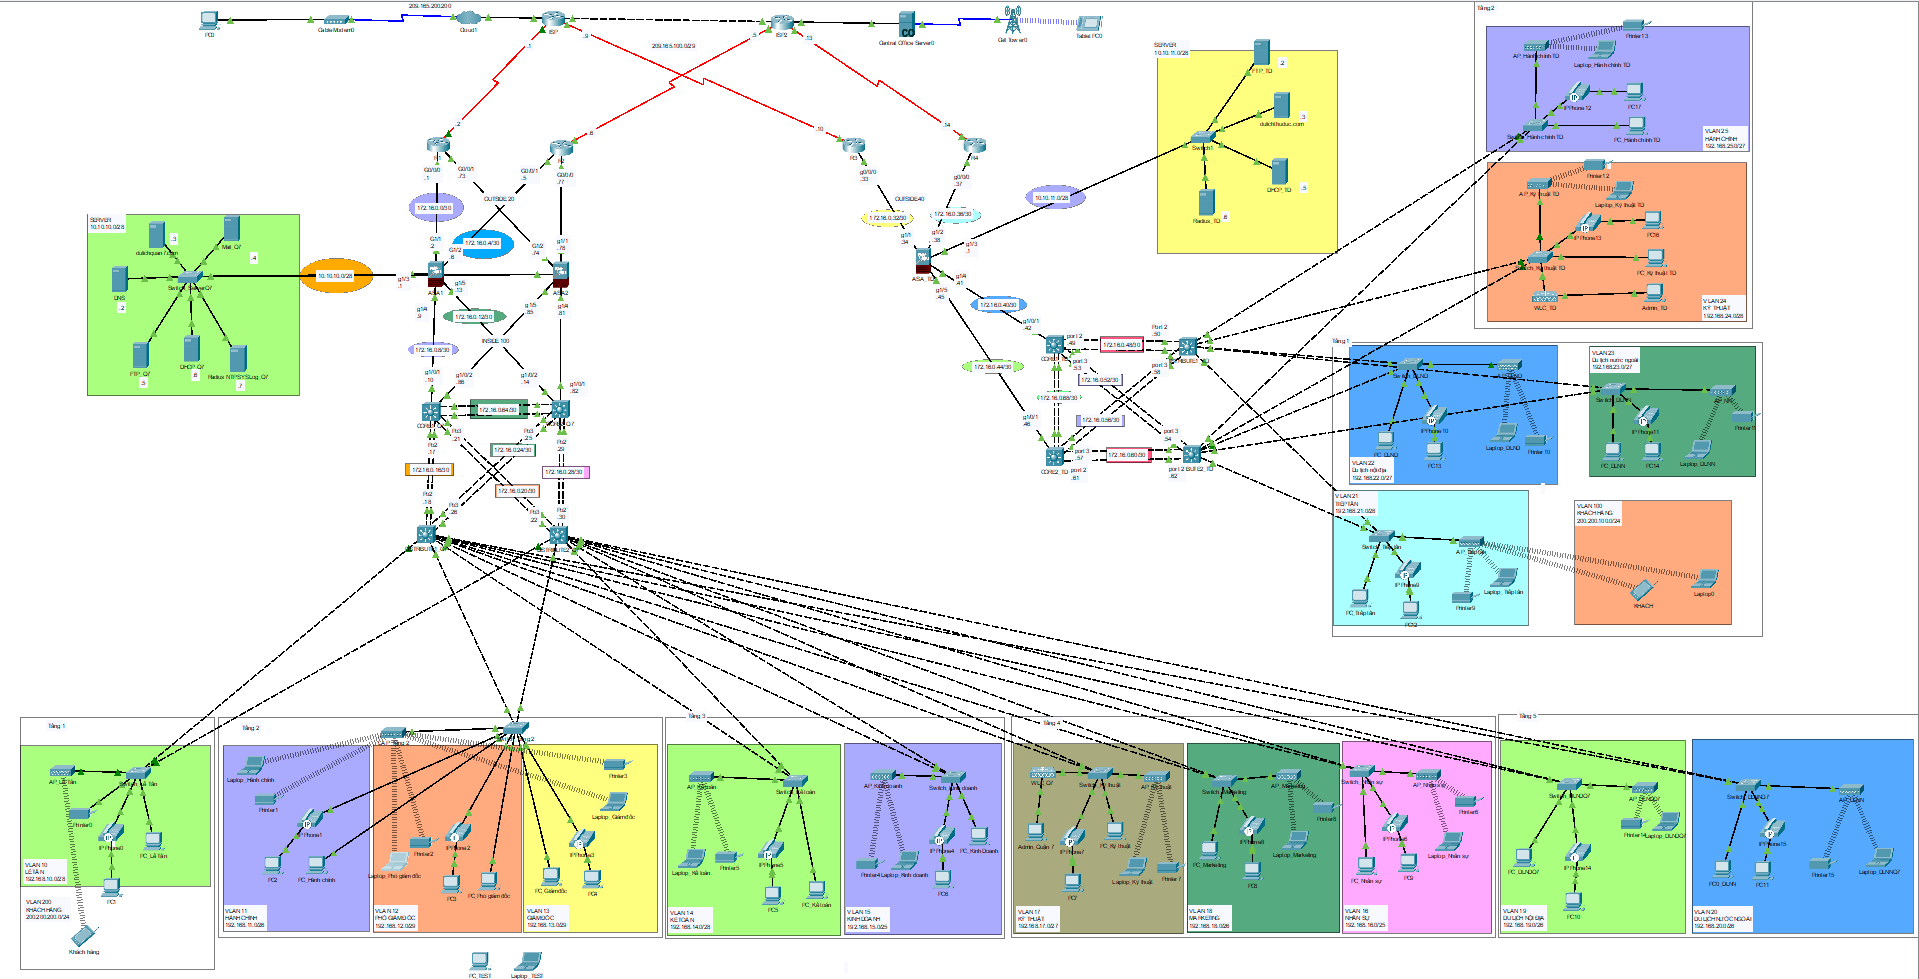
\includegraphics[width=16cm, height=10cm]{img/logic.png}
    \caption{Sơ đồ luận lý}
    \label{hinh21}
\end{figure}
\subsection{Sơ đồ vật lý}
\begin{figure}[H]
    \centering
    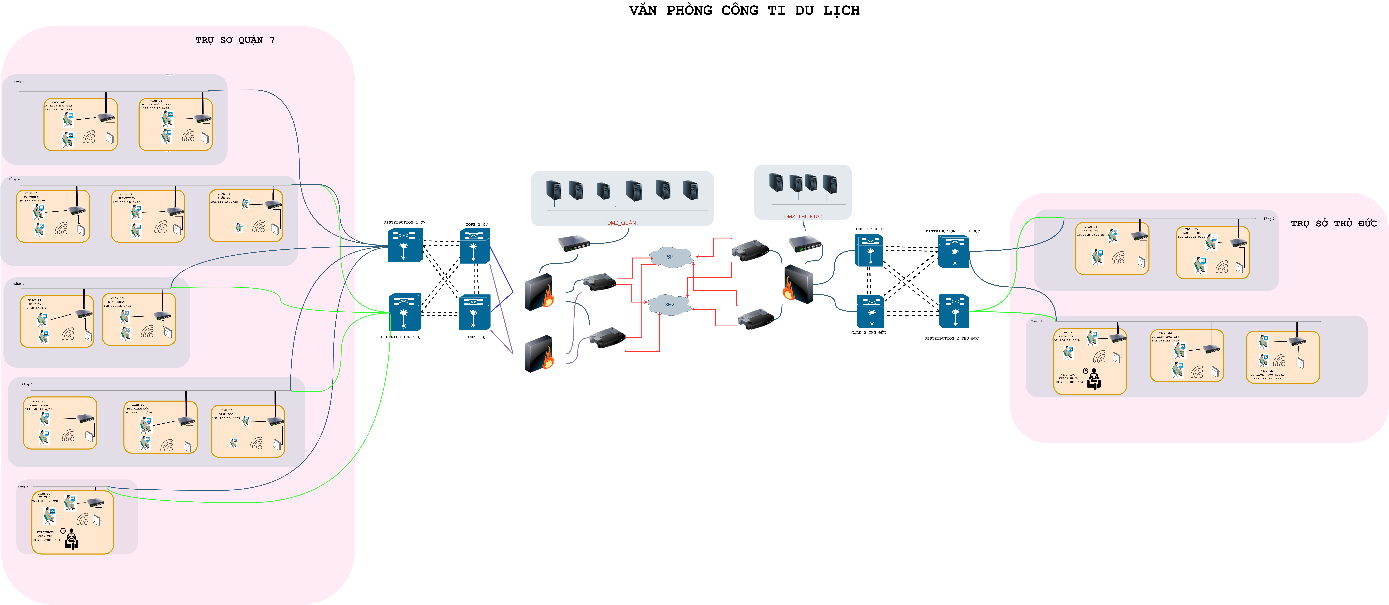
\includegraphics[width=16cm, height=12cm]{img/physical.drawio.png}
    \caption{Sơ đồ vật lý}
    \label{hinh22 }
\end{figure}
\subsection{Sơ đồ lắp đặt tủ Rack}
\begin{figure}[H]
    \centering
    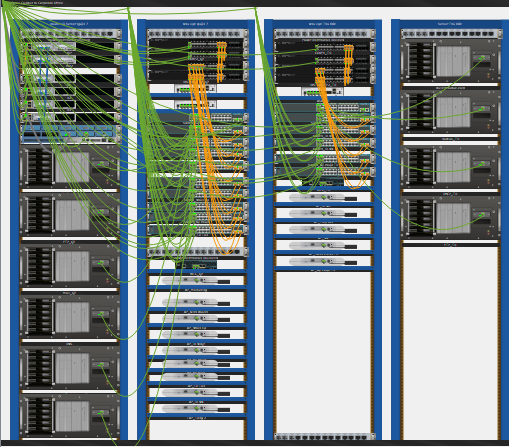
\includegraphics[width=16cm, height=14cm]{img/rack.png}
    \caption{Sơ đồ tủ Rack}
    \label{hinh23}
\end{figure}

\newpage
\section*{CHƯƠNG 3 - THÔNG TIN CÀI ĐẶT CẤU HÌNH HỆ THỐNG}
\addcontentsline{toc}{section}{\numberline{} CHƯƠNG 3 - THÔNG TIN CÀI ĐẶT CẤU HÌNH HỆ THỐNG}
\setcounter{section}{3}
\setcounter{subsection}{0}
\setcounter{figure}{0}
\setcounter{table}{0}
\subsection{Thông tin kết nối port trong hệ thống}
\begin{center}
\def\arraystretch{2.1}\begin{longtable}{|p{0.3\textwidth}|p{0.14\textwidth}|p{0.15\textwidth}|p{0.12\textwidth}|p{0.15 \textwidth}|}


\hline \textbf{Source to destination }    &      \textbf{Sources Interface }    &      \textbf{Destination Interface }    &    \textbf{Protocol } &     \textbf{Trunking/ vlan }\\ \hline
\endfirsthead



\hline \textbf{Source to destination } &  \textbf{Sources Interface } &  \textbf{Destination Interface } &  \textbf{Protocol } &  \textbf{Trunking/ vlan} \\ \hline
\endhead


\endfoot


\endlastfoot


\hline WEB\_Q7 to Switch\_ServerQ7     &     Fa     &     Fa/7    &  Ethernet  &   \\
\hline DNS to Switch\_ServerQ7        &     Fa     &     Fa/1    &  Ethernet  &   \\
\hline Mail\_Q7 to Switch\_ServerQ7     &     Fa     &     Fa/3    &  Ethernet  &   \\
\hline FTP\_Q7 to Switch\_ServerQ7     &     Fa     &     Fa/4    &  Ethernet  &   \\
\hline DHCP to Switch\_ServerQ7        &     Fa     &     Fa/5    &  Ethernet  &   \\
\hline Radius/NTP/SYSLog to Switch\_ServerQ7      &     Fa     &     Fa/6    &  Ethernet  &   \\
\hline ASA1 to Switch\_ServerQ7       &     Giga1/3     &     Giga0/1    &  Ethernet  &   \\
\hline ASA1 to Router1                &     Giga1/1     &     Giga0/0/0    &  Ethernet  &   \\
\hline ASA1 to Router2                &     Giga1/2     &     Giga0/0/1    &  Ethernet  &   \\
\hline ASA1 to CORE1\_Q7              &     Giga1/4     &     Giga1/0/1    &  Ethernet  &   \\
\hline ASA1 to CORE2\_Q7              &     Giga1/5     &     Giga1/0/2    &  Ethernet  &   \\
\hline ASA2 to Switch\_ServerQ7        &     Giga1/3     &     Giga0/2    &  Ethernet  &   \\
\hline ASA2 to Router1               &     Giga1/2     &     Giga0/0/1    &  Ethernet  &   \\
\hline ASA2 to Router2               &     Giga1/1     &     Giga0/0/0    &  Ethernet  &   \\
\hline ASA2 to CORE1\_Q7               &     Giga1/5     &     Giga1/0/2    &  Ethernet  &   \\
\hline ASA2 to CORE2\_Q7              &     Giga1/4     &     Giga1/0/1    &  Ethernet  &   \\
\hline CORE1\_Q7 to CORE2\_Q7         &     Giga1/0/23     &     Giga1/0/23    &  Ethernet  &  Port-Channel  \\
\hline CORE1\_Q7 to CORE2\_Q7           &     Giga1/0/24     &     Giga1/0/24    &  Ethernet  &  Port-Channel  \\
\hline CORE1\_Q7 to DISTRIBUTE1\_Q7     &     Giga1/0/19     &     Giga1/0/19    &  Ethernet  &  Port-Channel  \\
\hline CORE1\_Q7 to DISTRIBUTE1\_Q7     &     Giga1/0/20     &     Giga1/0/20    &  Ethernet  &  Port-Channel  \\
\hline CORE1\_Q7 to DISTRIBUTE2\_Q7     &     Giga1/0/21     &     Giga1/0/21    &  Ethernet  &  Port-Channel  \\
\hline CORE1\_Q7 to DISTRIBUTE2\_Q7    &     Giga1/0/22     &     Giga1/0/22    &  Ethernet  &  Port-Channel  \\
\hline CORE2\_Q7 to DISTRIBUTE1\_Q7    &     Giga1/0/21     &     Giga1/0/21    &  Ethernet  &  Port-Channel  \\
\hline CORE2\_Q7 to DISTRIBUTE1\_Q7    &     Giga1/0/22     &     Giga1/0/22    &  Ethernet  &  Port-Channel  \\
\hline CORE2\_Q7 to DISTRIBUTE2\_Q7    &     Giga1/0/19     &     Giga1/0/19    &  Ethernet  &  Port-Channel  \\
\hline CORE2\_Q7 to DISTRIBUTE2\_Q7     &     Giga1/0/20     &     Giga1/0/20    &  Ethernet  &  Port-Channel  \\
\hline DISTRIBUTE1\_Q7 to Switch\_Lễ Tân     &     Giga1/0/1     &     Giga0/1    &  Ethernet  &  TRUNKING  \\
\hline DISTRIBUTE1\_Q7 to Switch\_Tầng 2     &     Giga1/0/2     &     Giga0/1    &  Ethernet  &  TRUNKING  \\
\hline DISTRIBUTE1\_Q7 to Switch\_Kế Toán     &     Giga1/0/3     &     Giga0/1    &  Ethernet  &  TRUNKING  \\
\hline DISTRIBUTE1\_Q7 to Switch\_Kinh Doanh     &     Giga1/0/4     &     Giga0/1    &  Ethernet  &  TRUNKING  \\
\hline DISTRIBUTE1\_Q7 to Switch\_Kỹ Thuật     &     Giga1/0/5     &     Giga0/1    &  Ethernet  &  TRUNKING  \\
\hline DISTRIBUTE1\_Q7 to Switch\_Marketing     &     Giga1/0/6     &     Giga0/1    &  Ethernet  &  TRUNKING  \\
\hline DISTRIBUTE1\_Q7 to Switch\_Nhân sự     &     Giga1/0/7     &     Giga0/1    &  Ethernet  &  TRUNKING  \\
\hline DISTRIBUTE1\_Q7 to Switch\_DLNDQ7    &     Giga1/0/8     &     Giga0/1    &  Ethernet  &  TRUNKING  \\
\hline DISTRIBUTE1\_Q7 to Switch\_DLNNQ7    &     Giga1/0/9     &     Giga0/1    &  Ethernet  &  TRUNKING  \\
\hline DISTRIBUTE2\_Q7 to Switch\_Lễ Tân     &     Giga1/0/1     &     Giga0/2    &  Ethernet  &  TRUNKING  \\
\hline DISTRIBUTE2\_Q7 to Switch\_Tầng 2    &     Giga1/0/2     &     Giga0/2    &  Ethernet  &  TRUNKING  \\
\hline DISTRIBUTE2\_Q7 to Switch\_Kế Toán    &     Giga1/0/3     &     Giga0/2    &  Ethernet  &  TRUNKING  \\
\hline DISTRIBUTE2\_Q7 to Switch\_Kinh Doanh     &     Giga1/0/4     &     Giga0/2    &  Ethernet  &  TRUNKING  \\
\hline DISTRIBUTE2\_Q7 to Switch\_Kỹ Thuật    &     Giga1/0/5     &     Giga0/2    &  Ethernet  &  TRUNKING  \\
\hline DISTRIBUTE2\_Q7 to Switch\_Marketing    &     Giga1/0/6     &     Giga0/2    &  Ethernet  &  TRUNKING  \\
\hline DISTRIBUTE2\_Q7 to Switch\_Nhân sự    &     Giga1/0/7     &     Giga0/2    &  Ethernet  &  TRUNKING  \\
\hline DISTRIBUTE2\_Q7 to Switch\_DLNDQ7     &     Giga1/0/8     &     Giga0/2    &  Ethernet  &  TRUNKING  \\
\hline DISTRIBUTE2\_Q7 to Switch\_DLNNQ7     &     Giga1/0/9     &     Giga0/2    &  Ethernet  &  TRUNKING  \\
\hline Switch\_Lễ Tân to PC\_Lễ Tân    &     Fa/1     &     Fa    &  Ethernet  &  VLAN  \\
\hline Switch\_Lễ Tân to Printer0    &     Fa/2     &     Fa    &  Ethernet  &  VLAN  \\
\hline Switch\_Tầng 2 to PC\_Hành Chính     &     Fa/2     &     Fa    &  Ethernet  &  VLAN  \\
\hline Switch\_Tầng 2 to PC\_Phó Giám Đốc     &     Fa/3     &     Fa    &  Ethernet  &  VLAN  \\
\hline Switch\_Tầng 2 to PC\_Giám Đốc     &     Fa/1     &     Fa    &  Ethernet  &  VLAN  \\
\hline Switch\_Kế Toán to PC\_Giám Đốc     &     Fa/1     &     Fa    &  Ethernet  &  VLAN  \\
\hline Switch\_Kinh Doanh to PC\_Giám Đốc     &     Fa/1     &     Fa    &  Ethernet  &  VLAN  \\
\hline Switch\_Kỹ Thuật to PC\_Kỹ Thuật     &     Fa/1     &     Fa    &  Ethernet  &  VLAN  \\
\hline Switch\_Kỹ Thuật to Kỹ Thuật     &     Fa/4     &     Fa    &  Ethernet  &  VLAN  \\
\hline Switch\_Kỹ Thuật to Wireless LAN Controller\_ Q7     &     Fa/3     &     Giga1    &  Ethernet  &  VLAN  \\
\hline Wireless LAN Controller\_ Q7 to Admin\_Quận 7      &     Giga2     &     Fa    &  Ethernet  &   \\
\hline Switch\_Marketing to PC\_Marketing     &     Fa/1     &     Fa    &  Ethernet  &  VLAN  \\
\hline Switch\_Nhân sự to PC\_Nhân sự    &     Fa/1     &     Fa    &  Ethernet  &  VLAN  \\
\hline Switch\_DLNDQ7 to PC\_DLNDQ7     &     Fa/1     &     Fa    &  Ethernet  &  VLAN  \\
\hline Switch\_DLNNQ7 to PC0\_DLNN     &     Fa/1     &     Fa    &  Ethernet  &  VLAN  \\
\hline AP\_Lễ Tân to Switch\_Lễ Tân    &     Giga0     &     Fa/3    &  Ethernet  &  TRUNKING  \\
\hline LAP\_Tầng 2 to Switch\_Tầng 2    &     Giga0     &     Fa/4    &  Ethernet  &  TRUNKING  \\
\hline AP\_Kế Toán to Switch\_Kế Toán    &     Giga0     &     Fa/2    &  Ethernet  &  TRUNKING  \\
\hline AP\_Kinh Doanh to Switch\_Kinh Doanh     &     Giga0     &     Fa/2    &  Ethernet  &  TRUNKING  \\
\hline AP\_Kỹ Thuật to Switch\_Kỹ Thuật     &     Giga0     &     Fa/2    &  Ethernet  &  TRUNKING  \\
\hline AP\_Marketing to Switch\_Marketing     &     Giga0     &     Fa/2    &  Ethernet  &  TRUNKING  \\
\hline AP\_Nhân Sự to Switch\_Nhân Sự     &     Giga0     &     Fa/2    &  Ethernet  &  TRUNKING  \\
\hline AP\_DLNDQ7 to Switch\_DLNDQ7     &     Giga0     &     Fa/2    &  Ethernet  &  TRUNKING  \\
\hline AP\_DLNNQ7 to Switch\_DLNNQ7     &     Giga0     &     Fa/3    &  Ethernet  &  TRUNKING  \\
\hline Laptop\_Letan to AP\_Lễ Tân     &         &        &  Wireless  &   \\
\hline Khách hàng to AP\_Lễ Tân    &         &        &  Wireless  &   \\
\hline Laptop\_Hành chính to LAP\_Tầng 2     &         &        &  Wireless  &   \\
\hline Printer1 to LAP\_Tầng 2    &         &        &  Wireless  &   \\
\hline Laptop\_Phó giám đốc to LAP\_Tầng 2     &         &        &  Wireless  &   \\
\hline Printer2 to LAP\_Tầng 2    &         &        &  Wireless  &   \\
\hline Printer3 to LAP\_Tầng 2     &         &        &  Wireless  &   \\
\hline Laptop\_Giám đốc to LAP\_Tầng 2     &         &        &  Wireless  &   \\
\hline Laptop\_Kế toán to AP\_Kế Toán     &         &        &  Wireless  &   \\
\hline Printer5 to AP\_Kế Toán     &         &        &  Wireless  &   \\
\hline Printer4 to AP\_Kinh doanh     &         &        &  Wireless  &   \\
\hline Laptop\_Kinh doanh to AP\_Kinh doanh    &         &        &  Wireless  &   \\
\hline Laptop\_Kỹ thuật to AP\_Kỹ Thuật     &         &        &  Wireless  &   \\
\hline Printer7 to AP\_Kỹ Thuật     &         &        &  Wireless  &   \\
\hline Laptop\_Marketing to AP\_Marketing    &         &        &  Wireless  &   \\
\hline Printer8 to AP\_Marketing     &         &        &  Wireless  &   \\
\hline Laptop\_Nhân sự to AP\_Nhân Sự    &         &        &  Wireless  &   \\
\hline Printer6 to AP\_Nhân Sự     &         &        &  Wireless  &   \\
\hline Printer14 to AP\_DLNDQ7     &         &        &  Wireless  &   \\
\hline Laptop\_DLNDQ7 to AP\_DLNDQ7     &         &        &  Wireless  &   \\
\hline Printer15 to AP\_DLNN    &         &        &  Wireless  &   \\
\hline Laptop\_DLNNQ7 to AP\_DLNN   &         &        &  Wireless  &   \\
\hline ISP to Router1     &     Se0/1/0   &     Se0/1/0    &   &   \\
\hline ISP to Cloud1     &     Giga0/0/0    &     Ethernet6    &  Ethernet  &   \\
\hline Cable Modem0 to Cloud1     &     Port0     &     Coaxial7    &   &   \\
\hline Cable Modem0 to PC0      &     Port1     &     Fa    &  Ethernet  &   \\
\hline ISP to ISP2     &     Giga0/0/1     &     Giga0/0/1    &  Ethernet  &   \\
\hline ISP to Router3      &     Se0/1/1     &     Se0/1/0    &   &   \\
\hline ISP2 to Router2      &     Se0/1/0     &     Se0/1/0    &   &   \\
\hline ISP2 to Router4      &     Se0/1/1     &     Se0/1/0    &   &   \\
\hline ASA\_TD to Router3      &     Giga1/1     &     Giga0/0/0    &  Ethernet  &   \\
\hline ASA\_TD to Router4      &     Giga1/2     &     Giga0/0/1    &  Ethernet  &   \\
\hline ASA2 to Switch1      &     Giga1/3     &     Giga0/1    &  Ethernet  &   \\
\hline FTP\_TD to Switch1      &     Fa     &     Fa/1    &  Ethernet  &   \\
\hline WEB\_TD to Switch1      &     Fa     &     Fa/2    &  Ethernet  &   \\
\hline DHCP\_TD to Switch1      &     Fa     &     Fa/4    &  Ethernet  &   \\
\hline RADIUS\_TD to Switch1      &     Fa     &     Fa/5    &  Ethernet  &   \\
\hline ASA\_TD to CORE1\_TD      &     Giga1/4     &     Giga1/0/1    &  Ethernet  &   \\
\hline ASA\_TD to CORE2\_TD      &     Giga1/5     &     Giga1/0/1    &  Ethernet  &   \\
\hline CORE1\_TD to CORE2\_TD      &     Giga1/0/23     &     Giga1/0/23    &  Ethernet  &  Port-Channel  \\
\hline CORE1\_TD to CORE2\_TD      &     Giga1/0/24     &     Giga1/0/24    &  Ethernet  &  Port-Channel  \\
\hline CORE1\_TD to DISTRIBUTE1\_TD      &     Giga1/0/19     &     Giga1/0/19    &  Ethernet  &  Port-Channel  \\
\hline CORE1\_TD to DISTRIBUTE1\_TD      &     Giga1/0/20     &     Giga1/0/20    &  Ethernet  &  Port-Channel  \\
\hline CORE1\_TD to DISTRIBUTE2\_TD      &     Giga1/0/21     &     Giga1/0/21    &  Ethernet  &  Port-Channel  \\
\hline CORE1\_TD to DISTRIBUTE2\_TD      &     Giga1/0/22     &     Giga1/0/22    &  Ethernet  &  Port-Channel  \\
\hline CORE2\_TD to DISTRIBUTE1\_TD      &     Giga1/0/21     &     Giga1/0/21    &  Ethernet  &  Port-Channel  \\
\hline CORE2\_TD to DISTRIBUTE1\_TD      &     Giga1/0/22     &     Giga1/0/22    &  Ethernet  &  Port-Channel  \\
\hline CORE2\_TD to DISTRIBUTE2\_TD      &     Giga1/0/19     &     Giga1/0/19    &  Ethernet  &  Port-Channel  \\
\hline CORE2\_TD to DISTRIBUTE2\_TD      &     Giga1/0/20     &     Giga1/0/20    &  Ethernet  &  Port-Channel  \\
\hline DISTRIBUTE1\_TD to Switch\_Tiếp tân      &     Giga1/0/1     &     Giga0/1    &  Ethernet  &  TRUNKING  \\
\hline DISTRIBUTE1\_TD to Switch\_DLND      &     Giga1/0/2     &     Giga0/1    &  Ethernet  &  TRUNKING  \\
\hline DISTRIBUTE1\_TD to Switch\_DLNN      &     Giga1/0/3     &     Giga0/1    &  Ethernet  &  TRUNKING  \\
\hline DISTRIBUTE1\_TD to Switch\_Kỹ thuật TD      &     Giga1/0/4     &     Giga0/1    &  Ethernet  &  TRUNKING  \\
\hline DISTRIBUTE1\_TD to Switch\_Hành chính TD      &     Giga1/0/5     &     Giga0/1    &  Ethernet  &  TRUNKING  \\
\hline DISTRIBUTE2\_TD to Switch\_Tiếp tân      &     Giga1/0/1     &     Giga0/2    &  Ethernet  &  TRUNKING  \\
\hline DISTRIBUTE2\_TD to Switch\_DLND      &     Giga1/0/2     &     Giga0/2    &  Ethernet  &  TRUNKING  \\
\hline DISTRIBUTE2\_TD to Switch\_DLNN      &     Giga1/0/3     &     Giga0/2    &  Ethernet  &  TRUNKING  \\
\hline DISTRIBUTE2\_TD to Switch\_Kỹ thuật TD      &     Giga1/0/4     &     Giga0/2    &  Ethernet  &  TRUNKING  \\
\hline DISTRIBUTE2\_TD to Switch\_Hành chính TD      &     Giga1/0/5     &     Giga0/2    &  Ethernet  &  TRUNKING  \\
\hline Switch\_Tiếp tân to PC\_Tiếp tân      &     Fa/1     &     Fa    &  Ethernet  &  VLAN  \\
\hline Switch\_DLND to PC\_DLND      &     Fa/1     &     Fa    &  Ethernet  &  VLAN  \\
\hline Switch\_DLNN to PC\_DLNN      &     Fa/1     &     Fa    &  Ethernet  &  VLAN  \\
\hline Switch\_Kỹ thuật TD to Ky Thuat TD      &     Fa/4     &     Fa    &  Ethernet  &  VLAN  \\
\hline Switch\_Kỹ thuật TD to PC\_Kỹ thuật TD      &     Fa/1     &     Fa    &  Ethernet  &  VLAN  \\
\hline Switch\_Kỹ thuật TD to WLC\_TD      &     Fa/3     &     Giga1    &  Ethernet  &  VLAN  \\
\hline WLC\_TD to Admin\_TD      &     Giga2     &     Fa    &  Ethernet  &   \\
\hline Switch\_Hành chính TD to PC\_Hành chính TD      &     Fa/1     &     Fa    &  Ethernet  &  VLAN  \\
\hline AP\_Tiếp tân to Switch\_Tiếp tân      &     Giga0     &     Fa/2    &  Ethernet  &  TRUNKING  \\
\hline AP\_DLND to Switch\_DLND      &     Giga0     &     Fa/2    &  Ethernet  &  TRUNKING  \\
\hline AP\_NN to Switch\_DLNN      &     Giga0     &     Fa/2    &  Ethernet  &  TRUNKING  \\
\hline AP\_Kỹ thuật TD to Switch\_Kỹ thuật TD      &     Giga0     &     Fa/2    &  Ethernet  &  TRUNKING  \\
\hline AP\_Hành chính TD to Switch\_Hành chính TD      &     Giga0     &     Fa/2    &  Ethernet  &  TRUNKING  \\
\hline Printer9 to AP\_Tiếp tân      &         &        &  Wireless  &   \\
\hline Laptop\_Tiếp tân to AP\_Tiếp tân      &         &        &  Wireless  &   \\
\hline KHACH to AP\_Tiếp tân      &         &        &  Wireless  &   \\
\hline Laptop0 to AP\_Tiếp tân      &         &        &  Wireless  &   \\
\hline Laptop\_DLND to AP\_DLND      &         &        &  Wireless  &   \\
\hline Printer10 to AP\_DLND      &         &        &  Wireless  &   \\
\hline Laptop\_DLNN to AP\_NN      &         &        &  Wireless  &   \\
\hline Printer11 to AP\_NN      &         &        &  Wireless  &   \\
\hline Laptop\_Kỹ thuật TD to AP\_Kỹ thuật TD      &         &        &  Wireless  &   \\
\hline Printer12 to AP\_Kỹ thuật TD      &         &        &  Wireless  &   \\
\hline Laptop\_Hành chính TD to AP\_Hành chính TD      &         &        &  Wireless  &   \\
\hline Printer13 to AP\_Hành chính TD      &         &        &  Wireless  &   \\
\hline


    \caption{Thông tin kết nối port trong hệ thống}
    \label{hinh31}
\end{longtable}

\end{center}



\subsection{Thông tin VLAN, Interface VLAN trong hệ thống}
\begin{center}
\def\arraystretch{2.1}\begin{longtable}{|p{0.05\textwidth}|p{0.16\textwidth}|p{0.08\textwidth}|p{0.1\textwidth}|p{0.06\textwidth}|p{0.16\textwidth}|p{0.28\textwidth}|}


\hline \textbf{STT } &  \textbf{VLAN Name } &  \textbf{VLAN ID } &  \textbf{Phòng Ban } &  \textbf{Mask} &  \textbf{Default gateway } &  \textbf{Ipv6} \\ \hline
\endfirsthead


\endhead


\endfoot


\endlastfoot

\hline 1 &	LETAN&	10&	Lễ tân&	/28&	192.168.10.1&	2001:db8:acad:a::1/64 \\
\hline 2 &	HANH CHINH&	11&	Hành chính&	/26&	192.168.11.1&	2001:db8:acad:b::1/64\\
\hline 3 &	PHOGIAM DOC&	12&	Phó giám đốc&	/29&	192.168.12.1&	2001:db8:acad:c::1/64\\
\hline 4 &	GIAMDOC&	13&	Giám đốc&	/29&	192.168.13.1&	2001:db8:acad:d::1/64\\
\hline 5 &	KETOAN&	14&	Kế toán&	/28&	192.168.14.1&	2001:db8:acad:e::1/64\\
\hline 6 &	KINH DOANH&	15&	Kinh doanh&	/25&	192.168.15.1&	2001:db8:acad:f::1/64\\
\hline 7 &	NHANSU &	16&	Nhân sự&	/25&	192.168.16.1&	2001:db8:acad:16:1/64\\
\hline 8 &	KYTHUAT&	17&	Kỹ thuật&	/27&	192.168.17.1&	2001:db8:acad:17::1/64\\
\hline 9 &	MARKETING&	18&	Marketing&	/26&	192.168.18.1&	2001:db8:acad:18::1/64\\
\hline 10 &	DULICH NOIDIA&	19&	Du lịch nội địa&	/26&	192.168.19.1&	2001:db8:acad:19::1/64\\
\hline 11 &	DULICH NUOCNGOAI&	20&	Du lịch nước ngoài&	/26&	192.168.20.1&	2001:db8:acad:20::1/64\\
\hline 12 &	KHACH HANG&	200&	Khách hàng&	/24&	200.200.200.1&	2001:db8:acad:200::1/64\\
\hline 13 &	TIEPTAN&	21&	Tiếp tân&	/28&	192.168.21.1&	2001:db8:acad:21::1/64\\
\hline 14 &	DULICH NOIDIA \_TD&	22&	Du lịch nội địa&	/27&	192.168.22.1&	2001:db8:acad:22::1/64\\
\hline 15 &	DULICH NUOCNGOAI \_TD&	23&	Du lịch nước ngoài&	/27&	192.168.23.1&	2001:db8:acad:23::1/64\\
\hline 16 &	KYTHUAT \_TD&	24&	Kỹ thuật&	/28&	192.168.24.1&	2001:db8:acad:24::1/64\\
\hline 17 &	HANHCHINH \_TD&	25&	Hành chính&	/27&	192.168.25.1&	2001:db8:acad:25::1/64\\
\hline 18 &	KHACH HANG\_TD&	100&	Khách hàng&	/24&	200.200.100.1&	2001:db8:acad:100::1/64\\
 
 
 \hline
   \caption{Thông tin VLAN, interface VLAN trong hệ thống}
    \label{hinh33}
\end{longtable}
   
\end{center}



\subsection{Thông tin thiết kế quy hoạch địa chỉ IP Planning}
\begin{center}
    \def\arraystretch{2.1}\begin{longtable}{|p{0.05\textwidth}|p{0.15\textwidth}|p{0.09\textwidth}|p{0.14\textwidth}|p{0.07\textwidth}|p{0.13\textwidth}|p{0.3\textwidth}|}
    
    
    \hline \textbf{STT} &\textbf{DEVICES} & \textbf{INTER FACE} &  \textbf{IPv4 ADDRESS} &  \textbf{Mask} &\textbf{NET} & \textbf{IPV6}\\ \hline 
    
    \endfirsthead
    
    
    
    \hline \textbf{STT} &\textbf{DEVICES} & \textbf{INTER FACE} &  \textbf{IPv4 ADDRESS} &  \textbf{Mask} &\textbf{NET} & \textbf{IPV6}\\ \hline 
    
    \endhead
    
       
    \endfoot
    
    
    \endlastfoot
        \hline  \multicolumn{7}{|c|}{I/QUẬN 7} \\
        \hline 1 &	ASA1\_Q7	&G1/1	&172.16.0.2	&/30	&172.16.0.0	&2001:db8:acad:172::2/64\\
        \hline 2 &	ASA1\_Q7	&G1/2	&172.16.0.6	&/30	&172.16.0.4	&2001:db8:acad:173::2/64\\
        \hline 3 &	ASA1\_Q7	&G1/3	&10.10.10.1	&/28	&10.10.10.0	&2001:DB8:BADC:A::1/64\\
        \hline 4 &	ASA1\_Q7	&G1/4	&172.16.0.9	&/30	&172.16.0.8	&2001:db8:acad:174::1/64\\
        \hline 5 &	ASA1\_Q7	&G1/5	&172.16.0.13	&/30	&172.16.0.12	&2001:db8:acad:175::1/64\\
        \hline 6 &	ASA2\_Q7	&G1/1	&172.16.0.78	&/30	&172.16.0.76	&2001:db8:acad:178::2/64\\
        \hline 7 &	ASA2\_Q7	&G1/2	&172.16.0.74	&/30	&172.16.0.72	&2001:db8:acad:177::2/64\\
        \hline 8 &	ASA2\_Q7	&G1/3	&10.10.10.1	&/28	&10.10.10.0	&2001:DB8:BADC:A::1/64\\
        \hline 9 &	ASA2\_Q7	&G1/4	&172.16.0.81	&/30	&172.16.0.80	&2001:db8:acad:180::1/64\\
        \hline 10 &	ASA2\_Q7	&G1/5	&172.16.0.85	&/30	&172.16.0.84	&2001:db8:acad:179::1/64\\
        \hline 11 &	CORE1\_Q7	&G1/0/1	&172.16.0.10	&/30	&172.16.0.8	&2001:db8:acad:174::2/64\\
        \hline 12 &	CORE1\_Q7	&G1/0/2	&172.16.0.86	&/30	&172.16.0.84	&2001:db8:acad:179::2/64\\
        \hline 13 &	CORE1\_Q7	&G1/0/23-24(Port 1)	&172.16.0.65	&/30	&172.16.0.64	&2001:db8:acad:185::1/64\\
        \hline 14 &	CORE1\_Q7	&G1/0/21-22 (Port 2)	&172.16.0.17	&/30	&172.16.0.16	&2001:db8:acad:181::1/64\\
        \hline 15 &	CORE1\_Q7	&G1/0/19-20 (Port 3)	&172.16.0.21	&/30	&172.16.0.20	&2001:db8:acad:182::1/64\\
        \hline 16 &	CORE2\_Q7	&G1/0/1	&172.16.0.82	&/30	&172.16.0.80	&2001:db8:acad:180::2/64\\
        \hline 17 &	CORE2\_Q7	&G1/0/2	&172.16.0.14	&/30	&172.16.0.12	&2001:db8:acad:175::2/64\\
        \hline 18 &	CORE2\_Q7	&G1/0/23-24(Port 1)	&172.16.0.66	&/30	&172.16.0.64	&2001:db8:acad:185::2/64\\
        \hline 19 &	CORE2\_Q7	&G1/0/21-22 (Port 2)	&172.16.0.29	&/30	&172.16.0.28	&2001:db8:acad:184::1/64\\
        \hline 20 &	CORE2\_Q7	&G1/0/19-20 (Port 3)	&172.16.0.25	&/30	&172.16.0.24	&2001:db8:acad:183::1/64\\
        \hline 21 &	Distributed 1\_Q7 	&G1/0/21-22 (Port 2)	&172.16.0.18	&/30	&172.16.0.16	&2001:db8:acad:181::2/64\\
        \hline 22&	Distributed 1\_Q7	&G1/0/19-20 (Port 3)	&172.16.0.26	&/30	&172.16.0.24	&2001:db8:acad:183::2/64\\
        \hline 23 &	Distributed 1\_Q7	&G1/0/1-9	&\multicolumn{4} {|c|}{Trunking/Passive Interface}		
        \hline 24 &	Distributed 2\_Q7	&G1/0/21-22 (Port 2)	&172.16.0.30	&/30	&172.16.0.28	&2001:db8:acad:184::2/64\\
        \hline 25 &	Distributed 2\_Q7 	&G1/0/19-20 (Port 3)	&172.16.0.22	&/30	&172.16.0.20	&2001:db8:acad:182::2/64\\
        \hline 26 &	Distributed 2\_Q7 	&G1/0/1-9	&\multicolumn{4} {|c|}{Trunking/Passive Interface}			
        \hline  \multicolumn{7}{|c|}{II/THỦ ĐỨC} \\
        \hline 1 	&ASA\_TD	&G1/1	&172.16.0.34	&/30	&172.16.0.32	&2001:db8:acad:186::2/64\\
        \hline 2 	&ASA\_TD	&G1/2	&172.16.0.38	&/30	&172.16.0.36	&2001:db8:acad:187::2/64\\
        \hline 3 	&ASA\_TD	&G1/3	&10.10.11.1	&/28	&10.10.11.0	&2001:DB8:BADC:B::1/64\\
        \hline 4 	&ASA\_TD	&G1/4	&172.16.0.41	&/30	&172.16.0.40	&2001:db8:acad:188::1/64\\
        \hline 5 	&ASA\_TD	&G1/5	&172.16.0.45	&/30	&172.16.0.44	&2001:db8:acad:189::1/64\\
        \hline 6 	&CORE1\_TD	&G1/0/1	&172.16.0.42	&/30	&172.16.0.40	&2001:db8:acad:188::2/64\\
        \hline 7 	&CORE1\_TD	&G1/0/23-24(Port 1)	&172.16.0.69	&/30	&172.16.0.68	&2001:db8:acad:194::1/64\\
        \hline 8 	&CORE1\_TD	&G1/0/21-22 (Port 2)	&172.16.0.49	&/30	&172.16.0.48	&2001:db8:acad:190::1/64\\
        \hline 9 	&CORE1\_TD	&G1/0/19-20 (Port 3)	&172.16.0.53	&/30	&172.16.0.52	&2001:db8:acad:191::1/64\\
        \hline 10 	&CORE2\_TD	&G1/0/1	&172.16.0.46	&/30	&172.16.0.44	&2001:db8:acad:189::2/64\\
        \hline 11 	&CORE2\_TD	&G1/0/23-24(Port 1)	&172.16.0.70	&/30	&172.16.0.68	&2001:db8:acad:194::2/64\\
        \hline 12 	&CORE2\_TD	&G1/0/21-22 (Port 2)	&172.16.0.61	&/30	&172.16.0.60	&2001:db8:acad:193::1/64\\
        \hline 13 	&CORE2\_TD	&G1/0/19-20 (Port 3)	&172.16.0.57	&/30	&172.16.0.56	&2001:db8:acad:192::1/64\\
        \hline 14 	&Distributed 1\_TD	&G1/0/21-22 (Port 2)	&172.16.0.50	&/30	&172.16.0.48	&2001:db8:acad:190::2/64\\
        \hline 15 	&Distributed 1\_TD	&G1/0/19-20 (Port 3)	&172.16.0.58	&/30	&172.16.0.56	&2001:db8:acad:192::1/64\\
        \hline 16 	&Distributed 1\_TD	&G1/0/1-5	&\multicolumn{4} {|c|}{Trunking/Passive Interface}		
        \hline 17 	&Distributed 2\_TD	&G1/0/21-22 (Port 2)	&172.16.0.62	&/30	&172.16.0.60	&2001:db8:acad:193::2/64\\
        \hline 18 	&Distributed 2\_TD	&G1/0/19-20 (Port 3)	&172.16.0.54	&/30	&172.16.0.52	&2001:db8:acad:191::2/64\\
        \hline 19 	&Distributed 2\_TD	&G1/0/1-5	&\multicolumn{4} {|c|}{Trunking/Passive Interface}		
        \hline  \multicolumn{7}{|c|}{III/ROUTER BIÊN VÀ INTERNET} \\
        \hline \multirow{2}{*}{1} &ISP1	&S0/1/0	&209.165 .100.1	&/30	&209.165 .100.0	&2001:db8:acad:209::1/64\\\cline{3-7}
		                          &     &S0/1/1	&209.165 .100.9	&/30	&209.165 .100.0	&2001:db8:acad:210::1/64\\\cline{3-7}
        \hline \multirow{2}{*}2   &ISP2	&S0/1/0	&209.165 .100.5	&/30	&209.165 .100.0	&2001:db8:acad:211::1/64\\\cline{3-7}
		                          &     &S0/1/1	&209.165 .100.13	&/30	&209.165 .100.0	&2001:db8:acad:212::1/64\\\cline{3-7}
        \hline \multirow{3}{*}3   &R1	&G0/0/0	&172.16.0.1	&/30	&172.16.0.0	&2001:db8:acad:172::1/64\\\cline{3-7}
                                  &     &G0/0/1	&172.16.0.73	&/30	&172.16.0.72	&2001:db8:acad:177::1/64\\\cline{3-7}
                                  &     &S0/1/0	&209.165 .100.2	&/30	&209.165 .100.0	&2001:db8:acad:209::2/64\\\cline{3-7}
        \hline \multirow{3}{*}4   &R2	&G0/0/0	&172.16.0.77	&/30	&172.16.0.76	&2001:db8:acad:178::1/64\\\cline{3-7}
                                  &     &G0/0/1	&172.16.0.5	&/30	&172.16.0.4	&2001:db8:acad:173::1/64\\\cline{3-7}
                                  &     &S0/1/0	&209.165 .100.6	&/30	&209.165 .100.0	&2001:db8:acad:211::2/64\\\cline{3-7}
        \hline \multirow{2}{*}5   &R3	&G0/0/0	&172.16.0.33	&/30	&172.16.0.32	&2001:db8:acad:186::1/64\\\cline{3-7}
		                          &     &S0/1/0	&209.165 .100.10	&/30	&209.165 .100.0	&2001:db8:acad:210::2/64\\\cline{3-7}
        \hline \multirow{2}{*}6   &R4	&G0/0/0	&172.16.0.37	&/30	&172.16.0.36	&2001:db8:acad:187::1/64\\\cline{3-7}
		                          &     &S0/1/0	&209.165. 100.14	&/30	&209.165 .100.0	&2001:db8:acad:212::2/64\\\cline{3-7}
        \hline
        \caption{Thông tin thiết kế quy hoạch địa chỉ IP planning}
        \label{hinh33a }
    \end{longtable}
    
    \end{center}
\newpage
\section*{CHƯƠNG 4 - CẤU HÌNH HẠ TẦNG}
\addcontentsline{toc}{section}{\numberline{} CHƯƠNG 4 - CẤU HÌNH HẠ TẦNG}
\setcounter{section}{4}
\setcounter{subsection}{0}
\setcounter{figure}{0}
\setcounter{table}{0}
\subsection{Cấu hình Interface}
\subsubsection{Khu vực Router biên và Internet}
\begin{figure}[H]
    \centering
    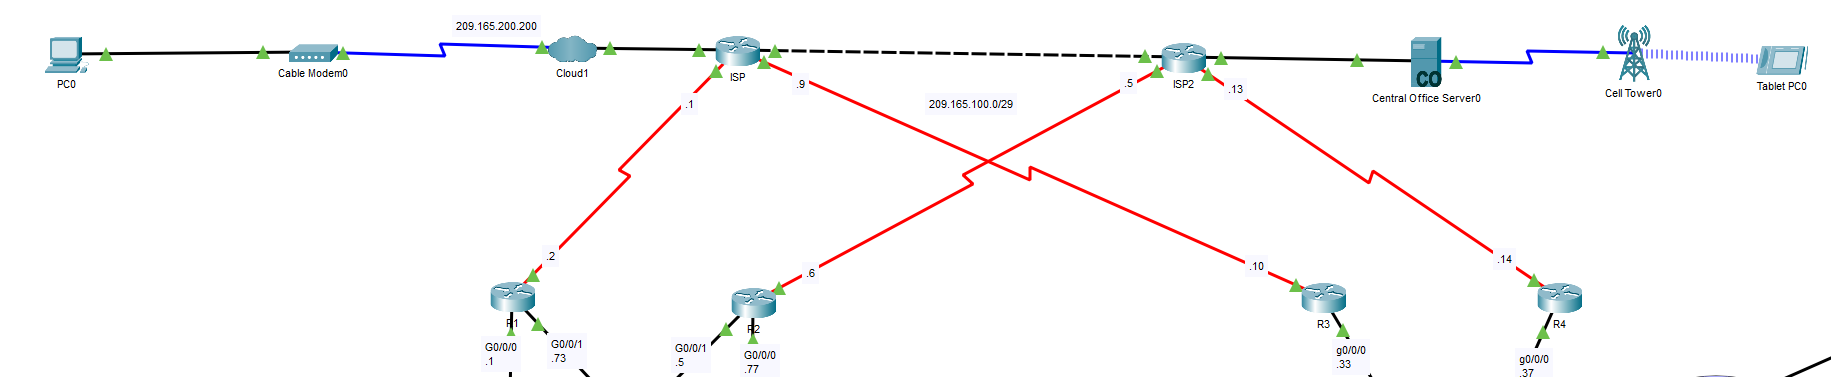
\includegraphics[width=16cm, height=6cm]{img/router.png}
    \caption{Khu vực Router biên và Internet}
    \label{hinh41}
\end{figure}
\hspace*{1cm}\textbf{a. Router R1} \\
\hspace*{2cm}\textit{hostname R1\\
\hspace*{2cm}int s0/1/0\\
\hspace*{2cm}ip address 209.165.100.2 255.255.255.252\\
\hspace*{2cm}ipv6 add 2001:db8:acad:209::2/64\\
\hspace*{2cm}ip nat out\\
\hspace*{2cm}clock rate 2000000\\
\hspace*{2cm}no shutdown\\
\hspace*{2cm}ex\\
\hspace*{2cm}int g0/0/0\\
\hspace*{2cm}ip address 172.16.0.89 255.255.255.252\\
\hspace*{2cm}ipv6 address 2001:db8:acad:172::1/64\\
\hspace*{2cm}ip nat in\\
\hspace*{2cm}no shutdown\\
\hspace*{2cm}exit\\
\hspace*{2cm}int g0/0/1\\
\hspace*{2cm}ip add 172.16.0.73 255.255.255.252\\
\hspace*{2cm}ipv6 address 2001:db8:acad:177::1/64\\
\hspace*{2cm}ip nat in\\
\hspace*{2cm}no shut\\
\hspace*{2cm}exit\\}
\hspace*{1cm}\textbf{b.Router R2} \\
\hspace*{2cm}\textit{hostname R2\\
\hspace*{2cm}int s0/1/0\\
\hspace*{2cm} ip address 209.165.100.6 255.255.255.252\\
\hspace*{2cm} ipv6 add 2001:db8:acad:211::2/64\\
\hspace*{2cm} ip nat out\\
\hspace*{2cm}clock rate 2000000\\
\hspace*{2cm}no shutdown\\
\hspace*{2cm}ex\\
\hspace*{2cm}int g0/0/0\\
\hspace*{2cm}ip address 172.16.0.77 255.255.255.252\\
\hspace*{2cm}ipv6 address 2001:db8:acad:178::1/64\\
\hspace*{2cm}ip nat in\\
\hspace*{2cm}no shutdown\\
\hspace*{2cm}exit\\
\hspace*{2cm}int g0/0/1\\
\hspace*{2cm}ip address 172.16.0.5 255.255.255.252\\
\hspace*{2cm}ipv6 address 2001:db8:acad:173::1/64\\
\hspace*{2cm}ip nat in\\
\hspace*{2cm}no shutdown\\
\hspace*{2cm}exit\\}
\hspace*{1cm}\textbf{c.Router R3} \\
\hspace*{2cm}\textit{hostname R3\\
\hspace*{2cm}int s0/1/0\\
\hspace*{2cm} ip address 209.165.100.10 255.255.255.252\\
\hspace*{2cm}ipv6 add 2001:db8:acad:210::2/64\\
\hspace*{2cm}ip nat out\\
\hspace*{2cm}ip ospf 1 area 0\\
\hspace*{2cm}no shut\\
\hspace*{2cm}exit\\
\hspace*{2cm}int g0/0/0\\
\hspace*{2cm}ip address 172.16.0.33 255.255.255.252\\
\hspace*{2cm}ipv6 address 2001:db8:acad:186::1/64\\
\hspace*{2cm}ip nat in\\
\hspace*{2cm}no shutdown\\
\hspace*{2cm}exit\\}
\hspace*{1cm}\textbf{d.Router R4} \\
\hspace*{2cm}\textit{hostname R4\\
\hspace*{2cm}int s0/1/0\\
\hspace*{2cm} ip address 209.165.100.14 255.255.255.252\\
\hspace*{2cm}ipv6 add 2001:db8:acad:212::2/64\\
\hspace*{2cm}ip nat out\\
\hspace*{2cm}clock rate 2000000\\
\hspace*{2cm}no shutdown\\
\hspace*{2cm}ex\\
\hspace*{2cm}int g0/0/0\\
\hspace*{2cm}ip address 172.16.0.37 255.255.255.252\\
\hspace*{2cm}ipv6 address 2001:db8:acad:187::1/64\\
\hspace*{2cm}ip nat in\\
\hspace*{2cm}no shutdown\\
\hspace*{2cm}ex\\}
\hspace*{1cm}\textbf{e.Router ISP 1} \\
\hspace*{2cm}\textit{hostname ISP\\
\hspace*{2cm}interface GigabitEthernet0/0/0\\
\hspace*{2cm}ip address 209.165.200.100 255.255.255.0\\
\hspace*{2cm}ip ospf priority 0\\
\hspace*{2cm}interface GigabitEthernet0/0/1\\
\hspace*{2cm}ip address 209.100.100.100 255.255.255.0\\
\hspace*{2cm}interface Serial0/1/0\\
\hspace*{2cm}ip address 209.165.100.1 255.255.255.252\\
\hspace*{2cm}ipv6 add 2001:db8:acad:209::1/64\\
\hspace*{2cm}interface Serial0/1/1\\
\hspace*{2cm}ip address 209.165.100.9 255.255.255.252\\
\hspace*{2cm}ipv6 add 2001:db8:acad:210::1/64\\
\hspace*{2cm}ex\\}
\hspace*{1cm}\textbf{f.Router ISP 2} \\
\hspace*{2cm}\textit{hostname ISP2\\
\hspace*{2cm}interface GigabitEthernet0/0/0\\
\hspace*{2cm}ip address 209.100.200.200 255.255.255.0\\
\hspace*{2cm}no shut\\
\hspace*{2cm}interface GigabitEthernet0/0/1\\
\hspace*{2cm}ip address 209.100.100.200 255.255.255.0\\
\hspace*{2cm}no shut\\
\hspace*{2cm}interface Serial0/1/0\\
\hspace*{2cm}ip address 209.165.100.5 255.255.255.252\\
\hspace*{2cm}ipv6 add 2001:db8:acad:211::1/64\\
\hspace*{2cm}interface Serial0/1/1\\
\hspace*{2cm}ip address 209.165.100.13 255.255.255.252\\
\hspace*{2cm}ipv6 add 2001:db8:acad:212::1/64\\
\hspace*{2cm}ex\\}
\subsubsection{Khu vực Quận 7 }
\hspace*{1cm}\textbf{a. Tường lửa ASA 1}\\
\hspace*{2cm}\textit{inter g1/1\\
\hspace*{2cm}nameif OUTSIDE\\
\hspace*{2cm}security-level 20\\
\hspace*{2cm}ip add 172.16.0.90 255.255.255.252\\
\hspace*{2cm}ipv6 add 2001:db8:acad:172::2/64\\
\hspace*{2cm}no shut \\
\hspace*{2cm}ex\\
\hspace*{2cm}inter g1/2\\
\hspace*{2cm}nameif OUTSIDE2\\
\hspace*{2cm}security-level 20\\
\hspace*{2cm}ip add 172.16.0.6 255.255.255.252\\
\hspace*{2cm}ipv6 add 2001:db8:acad:173::2/64\\
\hspace*{2cm}no shut \\
\hspace*{2cm}ex\\
\hspace*{2cm}inter g1/3\\
\hspace*{2cm}nameif DMZ\\
\hspace*{2cm}security-level 60\\
\hspace*{2cm}ip add 10.10.10.1 255.255.255.240\\
\hspace*{2cm}ipv6 add 2001:DB8:BADC:A::1/64\\
\hspace*{2cm}no shut\\
\hspace*{2cm}ex\\
\hspace*{2cm}inter g1/4\\
\hspace*{2cm}nameif INSIDE\\
\hspace*{2cm}security-level 100\\
\hspace*{2cm}ip add 172.16.0.9 255.255.255.252\\
\hspace*{2cm}ipv6 add 2001:db8:acad:174::1/64\\
\hspace*{2cm}no shut \\
\hspace*{2cm}ex\\
\hspace*{2cm}inter g1/5\\
\hspace*{2cm}nameif INSIDE2\\
\hspace*{2cm}security-level 100\\
\hspace*{2cm}ip add 172.16.0.13 255.255.255.252\\
\hspace*{2cm}ipv6 add 2001:db8:acad:175::1/64\\
\hspace*{2cm}no shut\\
\hspace*{2cm}ex\\}
\hspace*{1cm}\textbf{b. Tường lửa ASA 2}\\
\hspace*{2cm}\textit{inter g1/1\\
\hspace*{2cm}nameif OUTSIDE\\
\hspace*{2cm}security-level 20\\
\hspace*{2cm}ip add ip add 172.16.0.78 255.255.255.252\\
\hspace*{2cm}ipv6 add 2001:db8:acad:178::2/64\\
\hspace*{2cm}no shut \\
\hspace*{2cm}ex\\
\hspace*{2cm}inter g1/2\\
\hspace*{2cm}nameif OUTSIDE2\\
\hspace*{2cm}security-level 20\\
\hspace*{2cm}ip add 172.16.0.74 255.255.255.252\\
\hspace*{2cm}ipv6 add 2001:db8:acad:177::2/64\\
\hspace*{2cm}no shut \\
\hspace*{2cm}ex\\
\hspace*{2cm}inter g1/3\\
\hspace*{2cm}nameif DMZ\\
\hspace*{2cm}security-level 60\\
\hspace*{2cm}ip add 10.10.10.1 255.255.255.240\\
\hspace*{2cm}ipv6 add 2001:DB8:BADC:A::1/64\\
\hspace*{2cm}no shut\\
\hspace*{2cm}ex\\
\hspace*{2cm}inter g1/4\\
\hspace*{2cm}nameif INSIDE\\
\hspace*{2cm}security-level 100\\
\hspace*{2cm}ip add 172.16.0.81 255.255.255.252\\
\hspace*{2cm}ipv6 add 2001:db8:acad:180::1/64\\
\hspace*{2cm}no shut \\
\hspace*{2cm}ex\\
\hspace*{2cm}inter g1/5\\
\hspace*{2cm}nameif INSIDE2\\
\hspace*{2cm}security-level 100\\
\hspace*{2cm}ip add 172.16.0.85 255.255.255.252\\
\hspace*{2cm}ipv6 add 2001:db8:acad:179::1/64\\
\hspace*{2cm}no shut\\
\hspace*{2cm}ex\\}
\hspace*{1cm}\textbf{c. Switch Core 1}\\
\hspace*{2cm}\textit{hostname CORE1\_Q7\\
\hspace*{2cm}int g1/0/1\\
\hspace*{2cm}no sw\\
\hspace*{2cm}ip add 172.16.0.10 255.255.255.252\\
\hspace*{2cm}ipv6 add 2001:db8:acad:174::2/64\\
\hspace*{2cm}no shut\\}
\hspace*{1cm}\textbf{d. Switch Core 2}\\
\hspace*{2cm}\textit{hostname CORE2\_Q7\\
\hspace*{2cm}int g1/0/1\\
\hspace*{2cm}no sw\\
\hspace*{2cm}ip add 172.16.0.82 255.255.255.252\\
\hspace*{2cm}ipv6 add 2001:db8:acad:180::2/64\\
\hspace*{2cm}no shut\\}
\subsubsection{Khu vực Thủ Đức }
\hspace*{1cm}\textbf{a. Tường lửa ASA\_TD}\\
\hspace*{2cm}\textit{inter g1/1\\
\hspace*{2cm}nameif OUTSIDE\_TD\\
\hspace*{2cm}security-level 40\\
\hspace*{2cm}ip add ip add 172.16.0.34 255.255.255.252\\
\hspace*{2cm}ipv6 add 2001:db8:acad:180::2/64\\
\hspace*{2cm}no shut \\
\hspace*{2cm}ex\\
\hspace*{2cm}inter g1/2\\
\hspace*{2cm}nameif OUTSIDE2\_TD\\
\hspace*{2cm}security-level 40\\
\hspace*{2cm}ip add 172.16.0.38 255.255.255.252\\
\hspace*{2cm}ipv6 add 2001:db8:acad:181::2/64\\
\hspace*{2cm}no shut \\
\hspace*{2cm}ex\\
\hspace*{2cm}inter g1/3\\
\hspace*{2cm}nameif DMZ\_TD\\
\hspace*{2cm}security-level 60\\
\hspace*{2cm}ip add 10.10.11.1 255.255.255.240\\
\hspace*{2cm}ipv6 add 2001:DB8:BADC:B::1/64\\
\hspace*{2cm}no shut\\
\hspace*{2cm}ex\\
\hspace*{2cm}inter g1/4\\
\hspace*{2cm}nameif INSIDE\_TD\\
\hspace*{2cm}security-level 100\\
\hspace*{2cm}ip add 172.16.0.41 255.255.255.252\\
\hspace*{2cm}ipv6 add 2001:db8:acad:182::1/64\\
\hspace*{2cm}no shut \\
\hspace*{2cm}ex\\
\hspace*{2cm}inter g1/5\\
\hspace*{2cm}nameif INSIDE2\_TD\\
\hspace*{2cm}security-level 100\\
\hspace*{2cm}ip add 172.16.0.45 255.255.255.252\\
\hspace*{2cm}ipv6 add 2001:db8:acad:183::1/64\\
\hspace*{2cm}no shut\\
\hspace*{2cm}ex\\}
\hspace*{1cm}\textbf{b. Switch Core 1}\\
\hspace*{2cm}\textit{hostname CORE1\_TD\\
\hspace*{2cm}int g1/0/1\\
\hspace*{2cm}no sw\\
\hspace*{2cm}ip add 172.16.0.42 255.255.255.252\\
\hspace*{2cm}ipv6 add 2001:db8:acad:182::2/64\\
\hspace*{2cm}no shut\\}
\hspace*{1cm}\textbf{c. Switch Core 2}\\
\hspace*{2cm}\textit{hostname CORE2\_TD\\
\hspace*{2cm}int g1/0/1\\
\hspace*{2cm}no sw\\
\hspace*{2cm}ip add 172.16.0.46 255.255.255.252\\
\hspace*{2cm}ipv6 add 2001:db8:acad:183::2/64\\
\hspace*{2cm}no shut\\}
\subsection{Định tuyến động IPv4 và IPv6}
\hspace*{1cm}Để các Router và Switch có thể gửi gói tin cho nhau, chúng em sẽ sử dụng hai loại định tuyến động là OSPF và EIGRP.\\
\subsubsection{Router biên và Internet}

\renewcommand{\labelitemi}{$\blacksquare$}
\renewcommand\labelitemii{$\nabla$}
\renewcommand\labelitemiii{$\square$}
\begin{itemize}
      \item \textbf{Định tuyến IPv4}
      
      \begin{itemize}
        \item Router ISP 1
        \begin{itemize}
          \item \textit{router eigrp 10\\
                    	passive-interface GigabitEthernet0/0/0\\
                    	network 209.165.100.0 0.0.0.3\\
                    	network 209.165.100.8 0.0.0.3\\
                    	network 209.165.200.0\\
                    	network 209.100.100.0\\}
        
        \end{itemize}
        \item Router ISP 2
        \begin{itemize}
         \item \textit{router eigrp 10\\
                    	passive-interface GigabitEthernet0/0/0\\
                    	network 209.165.100.4 0.0.0.3\\
                    	network 209.165.100.12 0.0.0.3\\
                    	network 209.100.100.0\\}
         
          \end{itemize}
           \item Router R1
        \begin{itemize}
         \item \textit{ip routing\\
                        router eigrp 10\\
                        network 172.16.0.72 0.0.0.3\\
                        network 209.165.100.0 0.0.0.3\\
                        network 172.16.0.88 0.0.0.3\\
                        redistribute static metric 1000000 10 255 1 1500\\
                        exit\\
                        ip route 192.168.21.0 255.255.255.0 192.168.1.2\\
                        ip route 192.168.22.0 255.255.255.0 192.168.1.2\\
                        ip route 192.168.23.0 255.255.255.0 192.168.1.2\\
                        ip route 192.168.24.0 255.255.255.0 192.168.1.2\\
                        ip route 192.168.25.0 255.255.255.0 192.168.1.2\\
                        ip route 200.200.100.0 255.255.255.0 192.168.1.2\\
                        ip route 10.10.11.0 255.255.255.240 192.168.1.2\\
                        ip route 172.16.0.32 255.255.255.252 192.168.1.2\\
                        ip route 172.16.0.40 255.255.255.252 192.168.1.2\\
                        ip route 172.16.0.44 255.255.255.252 192.168.1.2\\
                        ip route 172.16.0.48 255.255.255.252 192.168.1.2\\
                        ip route 172.16.0.52 255.255.255.252 192.168.1.2\\
                        ip route 172.16.0.56 255.255.255.252 192.168.1.2\\
                        ip route 172.16.0.60 255.255.255.252 192.168.1.2\\}
         
          \end{itemize}
             \item Router R2
        \begin{itemize}
         \item \textit{ip routing\\
                        router eigrp 10\\
                        network 172.16.0.4 0.0.0.3\\
                        network 172.16.0.76 0.0.0.3\\
                        network 209.165.100.4 0.0.0.3\\
                        redistribute static metric 1000000 10 255 1 1500\\
                        exit\\
                        ip route 192.168.21.0 255.255.255.0 192.168.2.2\\
                        ip route 192.168.22.0 255.255.255.0 192.168.2.2\\
                        ip route 192.168.23.0 255.255.255.0 192.168.2.2\\
                        ip route 192.168.24.0 255.255.255.0 192.168.2.2\\
                        ip route 192.168.25.0 255.255.255.0 192.168.2.2\\
                        ip route 10.10.11.0 255.255.255.240 192.168.2.2\\
                        ip route 172.16.0.36 255.255.255.252 192.168.2.2\\
                        ip route 172.16.0.40 255.255.255.252 192.168.2.2\\
                        ip route 172.16.0.44 255.255.255.252 192.168.2.2\\
                        ip route 172.16.0.48 255.255.255.252 192.168.2.2\\
                        ip route 172.16.0.52 255.255.255.252 192.168.2.2\\
                        ip route 172.16.0.56 255.255.255.252 192.168.2.2\\
                        ip route 172.16.0.60 255.255.255.252 192.168.2.2\\
                        ip route 200.200.100.0 255.255.255.0 192.168.2.2\\}
         
          \end{itemize}
             \item Router R3
        \begin{itemize}
         \item \textit{ip routing\\
                        router eigrp 10\\
                        network 172.16.0.32 0.0.0.3\\
                        network 209.165.100.8 0.0.0.3\\
                        redistribute static metric 1000000 10 255 1 1500\\
                        exit\\
                        ip route 192.168.10.0 255.255.255.0 192.168.1.1\\
                        ip route 192.168.11.0 255.255.255.0 192.168.1.1\\
                        ip route 192.168.12.0 255.255.255.0 192.168.1.1\\
                        ip route 192.168.13.0 255.255.255.0 192.168.1.1\\
                        ip route 192.168.14.0 255.255.255.0 192.168.1.1\\
                        ip route 192.168.15.0 255.255.255.0 192.168.1.1\\
                        ip route 192.168.16.0 255.255.255.0 192.168.1.1\\
                        ip route 192.168.17.0 255.255.255.0 192.168.1.1\\
                        ip route 192.168.18.0 255.255.255.0 192.168.1.1\\
                        ip route 192.168.19.0 255.255.255.0 192.168.1.1\\
                        ip route 192.168.20.0 255.255.255.0 192.168.1.1\\
                        ip route 200.200.200.0 255.255.255.0 192.168.1.1\\
                        ip route 10.10.10.0 255.255.255.240 192.168.1.1\\}
         
          \end{itemize}
             \item Router R4
        \begin{itemize}
         \item \textit{ip routing\\
            router eigrp 10\\
            network 172.16.0.36 0.0.0.3\\
            network 209.165.100.12 0.0.0.3\\
            redistribute static metric 1000000 10 255 1 1500\\
            exit\\
            ip route 192.168.10.0 255.255.255.0 192.168.2.1\\
            ip route 192.168.11.0 255.255.255.0 192.168.2.1\\
            ip route 192.168.12.0 255.255.255.0 192.168.2.1\\
            ip route 192.168.13.0 255.255.255.0 192.168.2.1\\
            ip route 192.168.14.0 255.255.255.0 192.168.2.1\\
            ip route 192.168.15.0 255.255.255.0 192.168.2.1\\
            ip route 192.168.16.0 255.255.255.0 192.168.2.1\\
            ip route 192.168.17.0 255.255.255.0 192.168.2.1\\
            ip route 192.168.18.0 255.255.255.0 192.168.2.1\\
            ip route 192.168.19.0 255.255.255.0 192.168.2.1\\
            ip route 192.168.20.0 255.255.255.0 192.168.2.1\\
            ip route 200.200.200.0 255.255.255.0 192.168.2.1\\
            ip route 10.10.10.0 255.255.255.240 192.168.2.1\\}
         
          \end{itemize}
       \end{itemize}
     \hspace*{1cm} Trên Router ISP 1 và 2, chúng em sẽ sử dụng EIGRP để định tuyến Ipv4, sử dụng process-id là 10 và thêm các đường mạng xung quanh nó.\\
       \item \textbf{Định tuyến IPv6}
      \begin{itemize}
        \item Router ISP 1
        \begin{itemize}
          \item \textit{ipv6 unicast-routing\\
                    	ipv6 router ospf 20\\
                    	router-id 2.2.2.2\\
                    	exit\\
                    	int g0/0/0\\
                    	ipv6 ospf 20 area 0\\
                    	ex\\
                    	int g0/0/1\\
                    	ipv6 ospf 20 area 0\\
                    	ex\\
                    	int s0/1/0\\
                    	ipv6 ospf 20 area 0\\
                    	ex\\
                    	int s0/1/1\\
                    	ipv6 ospf 20 area 0\\
                    	ex\\}
       
        \end{itemize}
        \item Router ISP 2
        \begin{itemize}
         \item \textit{ipv6 unicast-routing\\
                        ipv6 router ospf 20\\
                        router-id 2.2.2.1\\
                        exit\\
                        int g0/0/0\\
                        ipv6 ospf 20 area 0\\
                        ex\\
                        int g0/0/1\\
                        ipv6 ospf 20 area 0\\
                        ex\\
                        int s0/1/0\\
                        ipv6 ospf 20 area 0\\
                        ex\\
                        int s0/1/1\\
                        ipv6 ospf 20 area 0\\
                        ex\\}
        
          \end{itemize}
            \item Router R1
           
        \begin{itemize}
         \item \textit{ipv6 unicast-routing\\
                        ipv6 router ospf 20\\
                        router-id 1.1.1.2\\
                        exit\\
                        int g0/0/0\\
                        ipv6 ospf 20 area 0\\
                        ex\\
                        int g0/0/1\\
                        ipv6 ospf 20 area 0\\
                        ex\\
                        int s0/1/0\\
                        ipv6 ospf 20 area 0\\
                        ex\\}
        
          \end{itemize}
             \item Router R2
           
        \begin{itemize}
         \item \textit{ipv6 unicast-routing\\
                        ipv6 router ospf 20\\
                        router-id 1.1.1.1\\
                        exit\\
                        int g0/0/0\\
                        ipv6 ospf 20 area 0\\
                        ex\\
                        int g0/0/1\\
                        ipv6 ospf 20 area 0\\
                        ex\\
                        int s0/1/0\\
                        ipv6 ospf 20 area 0\\
                        ex\\}
        
          \end{itemize}
             \item Router R3
           
        \begin{itemize}
         \item \textit{ipv6 unicast-routing\\
                        ipv6 router ospf 20\\
                        router-id 1.1.1.4\\
                        exit\\
                        int g0/0/0\\
                        ipv6 ospf 20 area 0\\
                        ex\\
                        int g0/0/1\\
                        ipv6 ospf 20 area 0\\
                        ex\\
                        int s0/1/0\\
                        ipv6 ospf 20 area 0\\
                        ex\\}
        
          \end{itemize}
             \item Router R4
           
        \begin{itemize}
         \item \textit{ipv6 unicast-routing\\
                        ipv6 router ospf 20\\
                        router-id 1.1.1.3\\
                        exit\\
                        int g0/0/0\\
                        ipv6 ospf 20 area 0\\
                        ex\\
                        int g0/0/1\\
                        ipv6 ospf 20 area 0\\
                        ex\\
                        int s0/1/0\\
                        ipv6 ospf 20 area 0\\
                        ex\\}
        
          \end{itemize}
       \end{itemize}
       \hspace*{0.25cm} Ở Router R1, chúng em sẽ sử dụng định tuyến EIGRP để định tuyến cho Ipv4 và OSPFv3 cho Ipv6, tương tự, cấu hình ở R2, R3 và R4\\
\end{itemize}

\subsubsection{Khu vực Quận 7}
\renewcommand{\labelitemi}{$\blacksquare$}
\renewcommand\labelitemii{$\nabla$}
\renewcommand\labelitemiii{$\square$}
\begin{itemize}
      \item \textbf{Định tuyến IPv4}
      
      \begin{itemize}
        \item Tường lửa ASA 1
        \begin{itemize}
          \item \textit{router eigrp 10\\
                    	network 172.16.0.4 0.0.0.3\\
                        network 172.16.0.8 0.0.0.3\\
                        network 172.16.0.12 0.0.0.3\\
                        network 10.10.10.0 0.0.0.15\\
                        network 172.16.0.88 0.0.0.3\\
                        passive-interface DMZ\\
                        ex\\}
        
        \end{itemize}
        \item Tường lửa ASA 2
        \begin{itemize}
         \item \textit{router eigrp 10\\
	network 172.16.0.72 0.0.0.3\\
network 172.16.0.76 0.0.0.3\\
network 172.16.0.80 0.0.0.3\\
network 172.16.0.84 0.0.0.3\\
network 10.10.10.0 0.0.0.15\\
passive-interface DMZ\\
ex\\}
         
          \end{itemize}
           \item Switch Core 1
        \begin{itemize}
         \item \textit{ip routing\\
                        router eigrp 10\\
                       network 172.16.0.8 0.0.0.3\\
                        network 172.16.0.16 0.0.0.3 \\
                        network 172.16.0.64 0.0.0.3 \\
                        network 172.16.0.20 0.0.0.3\\
                        network 172.16.0.84 0.0.0.3\\}
         
          \end{itemize}
             \item Switch Core 2
        \begin{itemize}
         \item \textit{ip routing\\
                        router eigrp 10\\
                        network 172.16.0.12 0.0.0.3\\
                        net 172.16.0.24 0.0.0.3 \\
                        net 172.16.0.28 0.0.0.3 \\
                        net 172.16.0.64 0.0.0.3\\
                        net 172.16.0.80 0.0.0.3 \\}
         
          \end{itemize}
             \item Switch Distribute 1
        \begin{itemize}
         \item \textit{ip routing\\
                        router eigrp 10\\
                        net 192.168.0.0 0.0.255.255 \\
                        net 200.200.200.0 0.0.0.255 \\
                        net 172.16.0.16 0.0.0.3 \\
                        net 172.16.0.24 0.0.0.3\\
                        passive-interface GigabitEthernet1/0/1\\
                        passive-interface GigabitEthernet1/0/2\\
                        passive-interface GigabitEthernet1/0/3\\
                        passive-interface GigabitEthernet1/0/4\\
                        passive-interface GigabitEthernet1/0/5\\
                        passive-interface GigabitEthernet1/0/6\\
                        passive-interface GigabitEthernet1/0/7\\
                        passive-interface GigabitEthernet1/0/8\\
                        passive-interface GigabitEthernet1/0/9\\}
         
          \end{itemize}
             \item Switch Distribute 2
        \begin{itemize}
         \item \textit{ip routing\\
            router eigrp 10\\
           net 172.16.0.28 0.0.0.3 \\
            net 172.16.0.20 0.0.0.3\\
            net 192.168.0.0 0.0.255.255\\
            net 200.200.200.0 \\
            passive-interface GigabitEthernet1/0/1\\
            passive-interface GigabitEthernet1/0/2\\
            passive-interface GigabitEthernet1/0/3\\
            passive-interface GigabitEthernet1/0/4\\
            passive-interface GigabitEthernet1/0/5\\
            passive-interface GigabitEthernet1/0/6\\
            passive-interface GigabitEthernet1/0/7\\
            passive-interface GigabitEthernet1/0/8\\
            passive-interface GigabitEthernet1/0/9\\}
         
          \end{itemize}
       \end{itemize}
     
       \item \textbf{Định tuyến IPv6}
      \begin{itemize}
        \item Tường lửa ASA 1
        \begin{itemize}
          \item \textit{ipv6 unicast-routing\\
                    	ipv6 router ospf 20\\
                        passive-interface DMZ\\
                        EX\\
                        int g1/1\\
                        ipv6 ospf 20 area 0\\
                        int g1/2\\
                        ipv6 ospf 20 area 0\\
                        int g1/3\\
                        ipv6 ospf 20 area 0\\
                        int g1/4\\
                        ipv6 ospf 20 area 0\\
                        int g1/5\\
                        ipv6 ospf 20 area 0\\
                        ex\\}
       
        \end{itemize}
        \item Tường lửa ASA 2
        \begin{itemize}
         \item \textit{ipv6 unicast-routing\\
                        ipv6 router ospf 20\\
                        passive-interface DMZ\\
                        EX\\
                        int g1/1\\
                        ipv6 ospf 20 area 0\\
                        int g1/2\\
                        ipv6 ospf 20 area 0\\
                        int g1/3\\
                        ipv6 ospf 20 area 0\\
                        int g1/4\\
                        ipv6 ospf 20 area 0\\
                        int g1/5\\
                        ipv6 ospf 20 area 0\\
                        ex\\}
        
          \end{itemize}
            \item Switch Core 1
           
        \begin{itemize}
         \item \textit{ipv6 unicast-routing\\
                       router-id 172.16.0.10\\
                        ex\\
                        int g1/0/1\\
                        ipv6 ospf 20 area 0\\
                        ex\\
                        int g1/0/2\\
                        ipv6 ospf 20 area 0\\
                        ex\\
                        int po 1\\
                        ipv6 ospf 20 area 0\\
                        ex\\
                        int po 2\\
                        ipv6 ospf 20 area 0\\
                        ex\\
                        int po 3\\
                        ipv6 ospf 20 area 0\\
                        ex\\}
        
          \end{itemize}
             \item Switch Core 2
           
        \begin{itemize}
         \item \textit{ipv6 unicast-routing\\
                       router-id 172.16.0.82\\
                        ex\\
                        int g1/0/1\\
                        ipv6 ospf 20 area 0\\
                        ex\\
                        int g1/0/2\\
                        ipv6 ospf 20 area 0\\
                        ex\\
                        int po 1\\
                        ipv6 ospf 20 area 0\\
                        ex\\
                        int po 2\\
                        ipv6 ospf 20 area 0\\
                        ex\\
                        int po 3\\
                        ipv6 ospf 20 area 0\\
                        ex\\}
        
          \end{itemize}
             \item Switch Distribute 1
           
        \begin{itemize}
         \item \textit{ipv6 unicast-routing\\
                        ipv6 router ospf 20\\
                       router-id 172.16.0.18\\
                         passive-interface GigabitEthernet1/0/1\\
                         passive-interface GigabitEthernet1/0/2\\
                         passive-interface GigabitEthernet1/0/3\\
                         passive-interface GigabitEthernet1/0/4\\
                         passive-interface GigabitEthernet1/0/5\\
                         passive-interface GigabitEthernet1/0/6\\
                         passive-interface GigabitEthernet1/0/7\\
                         passive-interface GigabitEthernet1/0/8\\
                         passive-interface GigabitEthernet1/0/9\\
                        int po 2\\
                        ipv6 ospf 20 area 0\\
                        int po 3\\
                        ipv6 ospf 20 area 0\\
                        int vlan 10\\
                        ipv6 ospf 20 area 0\\
                        int vlan 11\\
                        ipv6 ospf 20 area 0\\
                        int vlan 12\\
                        ipv6 ospf 20 area 0\\
                        int vlan 13\\
                        ipv6 ospf 20 area 0\\
                        int vlan 14\\
                        ipv6 ospf 20 area 0\\
                        int vlan 15\\
                        ipv6 ospf 20 area 0\\
                        int vlan 16\\
                        ipv6 ospf 20 area 0\\
                        int vlan 17\\
                        ipv6 ospf 20 area 0\\
                        int vlan 18\\
                        ipv6 ospf 20 area 0\\
                        int vlan 19\\
                        ipv6 ospf 20 area 0\\
                        int vlan 20\\
                        ipv6 ospf 20 area 0\\
                        int vlan 110\\
                        ipv6 ospf 20 area 0\\
                        int vlan 200\\
                        ipv6 ospf 20 area 0\\
                        ex\\}
\end{itemize}
             \item Switch Distribute 2
        \begin{itemize}
         \item \textit{ipv6 unicast-routing\\
                        ipv6 router ospf 20\\
                        router-id 172.16.0.30\\
                         passive-interface GigabitEthernet1/0/1\\
                         passive-interface GigabitEthernet1/0/2\\
                         passive-interface GigabitEthernet1/0/3\\
                         passive-interface GigabitEthernet1/0/4\\
                         passive-interface GigabitEthernet1/0/5\\
                         passive-interface GigabitEthernet1/0/6\\
                         passive-interface GigabitEthernet1/0/7\\
                         passive-interface GigabitEthernet1/0/8\\
                         passive-interface GigabitEthernet1/0/9\\
                        int po 2\\
                        ipv6 ospf 20 area 0\\
                        int po 3\\
                        ipv6 ospf 20 area 0\\
                        int vlan 10\\
                        ipv6 ospf 20 area 0\\
                        int vlan 11\\
                        ipv6 ospf 20 area 0\\
                        int vlan 12\\
                        ipv6 ospf 20 area 0\\
                        int vlan 13\\
                        ipv6 ospf 20 area 0\\
                        int vlan 14\\
                        ipv6 ospf 20 area 0\\
                        int vlan 15\\
                        ipv6 ospf 20 area 0\\
                        int vlan 16\\
                        ipv6 ospf 20 area 0\\
                        int vlan 17\\
                        ipv6 ospf 20 area 0\\
                        int vlan 18\\
                        ipv6 ospf 20 area 0\\
                        int vlan 19\\
                        ipv6 ospf 20 area 0\\
                        int vlan 20\\
                        ipv6 ospf 20 area 0\\
                        int vlan 110\\
                        ipv6 ospf 20 area 0\\
                        int vlan 200\\
                        ipv6 ospf 20 area 0\\
                        ex\\}
        
          \end{itemize}
       \end{itemize}
      
\end{itemize}



\subsubsection{Khu vực Thủ Đức}
\renewcommand{\labelitemi}{$\blacksquare$}
\renewcommand\labelitemii{$\nabla$}
\renewcommand\labelitemiii{$\square$}
\begin{itemize}
      \item \textbf{Định tuyến IPv4}
      
      \begin{itemize}
        \item Tường lửa ASA 
        \begin{itemize}
          \item \textit{router eigrp 10\\
                    	net 172.16.0.32 255.255.255.252 \\
                        net 172.16.0.36 255.255.255.252 \\
                        net 172.16.0.40 255.255.255.252 \\
                        net 172.16.0.44 255.255.255.252 \\
                        net 10.10.11.0 255.255.255.240 \\
                        passive-interface DMZ\_TD\\
                        ex\\}
        
        \end{itemize}
      
           \item Switch Core 1
        \begin{itemize}
         \item \textit{ip routing\\
                        router eigrp 10\\
                        network 172.16.0.40 0.0.0.3\\
                        network 172.16.0.48 0.0.0.3\\
                        network 172.16.0.52 0.0.0.3\\
                        network 172.16.0.68 0.0.0.3\\}
         
          \end{itemize}
             \item Switch Core 2
        \begin{itemize}
         \item \textit{ip routing\\
                        router eigrp 10\\
                        network 172.16.0.44 0.0.0.3\\
                        network 172.16.0.60 0.0.0.3\\
                        network 172.16.0.56 0.0.0.3\\
                        network 172.16.0.68 0.0.0.3\\}
         
          \end{itemize}
             \item Switch Distribute 1
        \begin{itemize}
         \item \textit{ip routing\\
                        router eigrp 10\\
                        net 172.16.0.48 0.0.0.3 \\
                        net 172.16.0.56 0.0.0.3 \\
                        net 200.200.100.0 0.0.0.255 \\
                        net 192.168.0.0 0.0.255.255 \\
                        passive-interface GigabitEthernet1/0/1\\
                        passive-interface GigabitEthernet1/0/2\\
                        passive-interface GigabitEthernet1/0/3\\
                        passive-interface GigabitEthernet1/0/4\\
                        passive-interface GigabitEthernet1/0/5\\}
         
          \end{itemize}
             \item Switch Distribute 2
        \begin{itemize}
         \item \textit{ip routing\\
            router eigrp 10\\
            network 172.16.0.60 0.0.0.3\\
            network 172.16.0.52 0.0.0.3\\
            network 192.168.0.0 0.0.255.255\\
            network 200.200.100.0\\
            passive-interface GigabitEthernet1/0/1\\
            passive-interface GigabitEthernet1/0/2\\
            passive-interface GigabitEthernet1/0/3\\
            passive-interface GigabitEthernet1/0/4\\
            passive-interface GigabitEthernet1/0/5\\}
         
          \end{itemize}
       \end{itemize}
     
       \item \textbf{Định tuyến IPv6}
      \begin{itemize}
        \item Tường lửa ASA 
        \begin{itemize}
          \item \textit{ipv6 unicast-routing\\
                    	ipv6 router ospf 20\\
                        passive-interface DMZ\_TD\\
                        EX\\
                        int g1/1\\
                        ipv6 ospf 20 area 0\\
                        int g1/2\\
                        ipv6 ospf 20 area 0\\
                        int g1/3\\
                        ipv6 ospf 20 area 0\\
                        int g1/4\\
                        ipv6 ospf 20 area 0\\
                        int g1/5\\
                        ipv6 ospf 20 area 0\\
                        ex\\}
       
        \end{itemize}
       
            \item Switch Core 1
           
        \begin{itemize}
         \item \textit{ipv6 unicast-routing\\
                       router-id 172.16.0.42\\
                        ex\\
                        int g1/0/1\\
                        ipv6 ospf 20 area 0\\
                        ex\\
                        int po 1\\
                        ipv6 ospf 20 area 0\\
                        ex\\
                        int po 2\\
                        ipv6 ospf 20 area 0\\
                        ex\\
                        int po 3\\
                        ipv6 ospf 20 area 0\\
                        ex\\
                       }
        
          \end{itemize}
             \item Switch Core 2
           
        \begin{itemize}
         \item \textit{ipv6 unicast-routing\\
                       router-id 172.16.0.46\\
                        ex\\
                        int g1/0/1\\
                        ipv6 ospf 20 area 0\\
                        ex\\
                        int po 1\\
                        ipv6 ospf 20 area 0\\
                        ex\\
                        int po 2\\
                        ipv6 ospf 20 area 0\\
                        ex\\
                        int po 3\\
                        ipv6 ospf 20 area 0\\
                        ex\\}
        
          \end{itemize}
             \item Switch Distribute 1
           
        \begin{itemize}
         \item \textit{ipv6 unicast-routing\\
                        ipv6 router ospf 20\\
                       router-id 172.16.0.50\\
                         passive-interface GigabitEthernet1/0/1\\
                         passive-interface GigabitEthernet1/0/2\\
                         passive-interface GigabitEthernet1/0/3\\
                         passive-interface GigabitEthernet1/0/4\\
                         passive-interface GigabitEthernet1/0/5\\
                        int po 2\\
                        ipv6 ospf 20 area 0\\
                        int po 3\\
                        ipv6 ospf 20 area 0\\
                        int vlan 21\\
                        ipv6 ospf 20 area 0\\
                        int vlan 22\\
                        ipv6 ospf 20 area 0\\
                        int vlan 23\\
                        ipv6 ospf 20 area 0\\
                        int vlan 24\\
                        ipv6 ospf 20 area 0\\
                        int vlan 25\\
                        ipv6 ospf 20 area 0\\
                        int vlan 111\\
                        ipv6 ospf 20 area 0\\
                        int vlan 100\\
                        ipv6 ospf 20 area 0\\
                        ex\\}
        
          \end{itemize}
             \item Switch Distribute 2
           
        \begin{itemize}
         \item \textit{ipv6 unicast-routing\\
                        ipv6 router ospf 20\\
                        router-id 172.16.0.62\\
                         passive-interface GigabitEthernet1/0/1\\
                         passive-interface GigabitEthernet1/0/2\\
                         passive-interface GigabitEthernet1/0/3\\
                         passive-interface GigabitEthernet1/0/4\\
                         passive-interface GigabitEthernet1/0/5\\
                        int po 2\\
                        ipv6 ospf 20 area 0\\
                        int po 3\\
                        ipv6 ospf 20 area 0\\
                        int vlan 21\\
                        ipv6 ospf 20 area 0\\
                        int vlan 22\\
                        ipv6 ospf 20 area 0\\
                        int vlan 23\\
                        ipv6 ospf 20 area 0\\
                        int vlan 24\\
                        ipv6 ospf 20 area 0\\
                        int vlan 25\\
                        ipv6 ospf 20 area 0\\
                        int vlan 111\\
                        ipv6 ospf 20 area 0\\
                        int vlan 100\\
                        ipv6 ospf 20 area 0\\
                        ex\\}
        
          \end{itemize}
       \end{itemize}
      
\end{itemize}

\subsection{Cấu hình khu vực DMZ }
\subsubsection{DNS Server}
\hspace*{0.25cm}Chúng ta sẽ sử dụng Server DNS để đăng ký tên miền cho cả hai chi nhánh là quận 7 và Thủ Đức.\\
\begin{figure}[H]
    \centering
    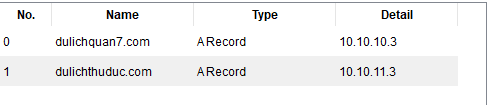
\includegraphics[width=16cm, height=4cm]{img/4.4.1a.png}
    \caption{Đăng ký 2 tên miền cho hai trụ sở}
    \label{hinh441a}
\end{figure}
\begin{figure}[H]
    \centering
    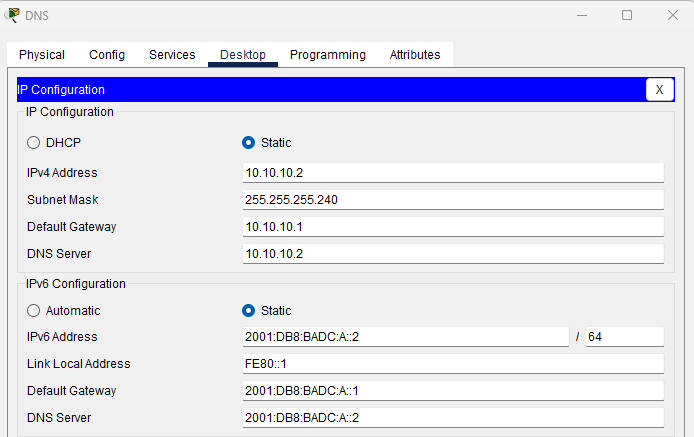
\includegraphics[width=17cm, height=14cm]{img/4.1.1b.png}
    \caption{Cấu hình địa chỉ Ipv4 và Ipv6 cho DNS Server}
    \label{hinh441b}
\end{figure}
\subsubsection{WEB Server }
\begin{figure}[H]
    \centering
    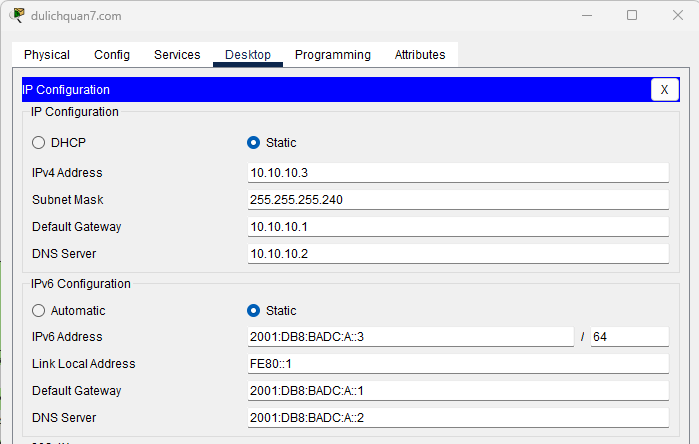
\includegraphics[width=16cm, height=14cm]{img/4.2.1.png}
    \caption{Cấu hình địa chỉ Ipv4 và Ipv6 cho Web Server trụ sở Quận 7}
    \label{hinh421}
    
\end{figure}


\begin{figure}[H]
    \centering
    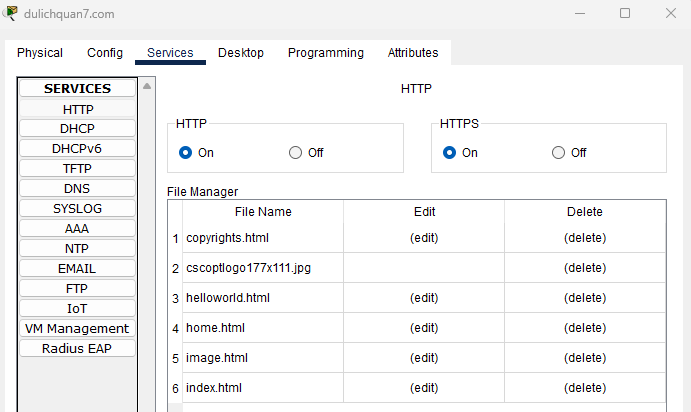
\includegraphics[width=17cm, height=12cm]{img/4.2.1b.png}
    \caption{ Bật dịch vụ HTTP}
    \label{hinh421b}
\end{figure}
Truy cập trang web đã tạo tên miền: \\

\begin{figure}[H]
    \centering
    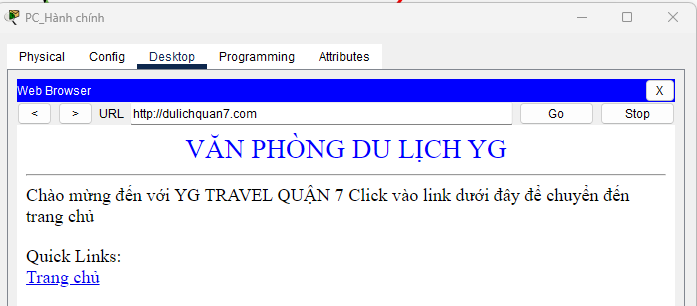
\includegraphics[width=16cm, height=8cm]{img/4.2.1d.png}
    \caption{Truy cập đến trang web thành công.}
    \label{hinh421d}
\end{figure}
\hspace*{0.25cm}Ngoài ra, ở máy chủ Web, chúng ta sẽ cài đặt tên miền với địa chỉ public, để các địa chỉ ngoài LAN có thể truy cập vào web.\\
\begin{figure}[H]
    \centering
    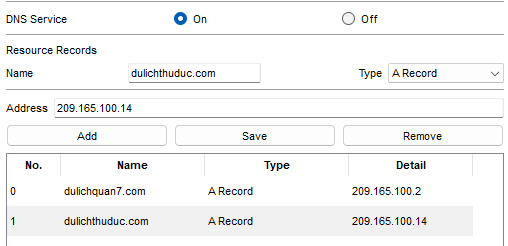
\includegraphics[width=16cm, height=8cm]{img/4.4.2d.png}
    \caption{Đăng ký tên miền bằng địa chỉ public }
    \label{hinh441a}
\end{figure}
\subsubsection{Mail Server}
\begin{figure}[H]
    \centering
    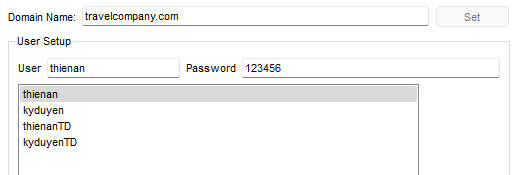
\includegraphics[width=16cm, height=6cm]{img/4.2.2a.png}
    \caption{Bật dịch vụ Mail Server}
    \label{hinh422a}
\end{figure}
\begin{figure}[H]
    \centering
    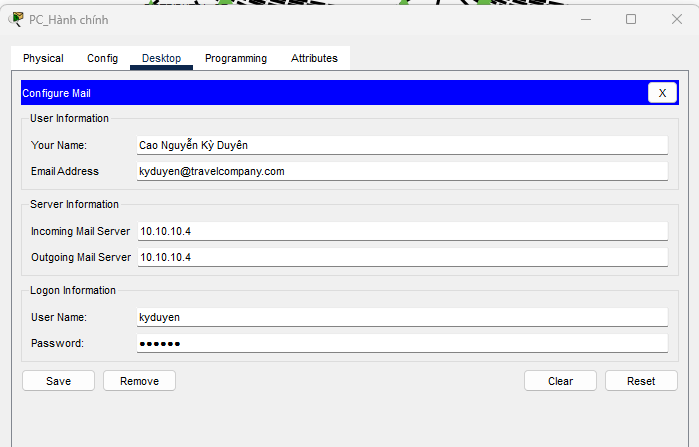
\includegraphics[width=16cm, height=10cm]{img/4.2.2b.png}
    \caption{Cấu hình email cho máy phòng Hành chính.}
    \label{hinh422b}
\end{figure}
\begin{figure}[H]
    \centering
    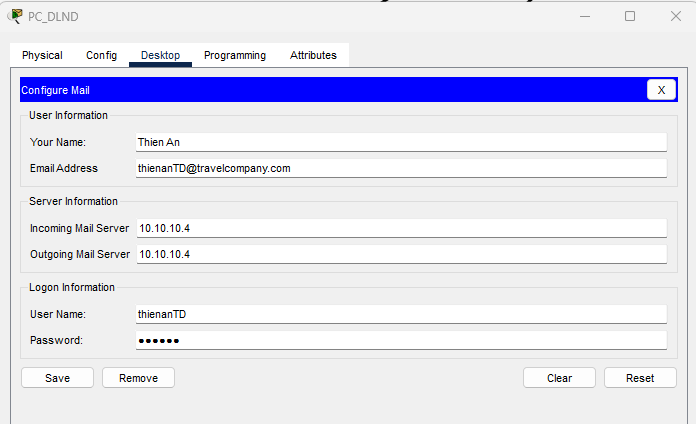
\includegraphics[width=16cm, height=10cm]{img/4.2.2c.png}
    \caption{Cấu hình email cho máy phòng Du lịch nội địa}
    \label{hinh422c}
\end{figure}

\begin{figure}[H]
    \centering
    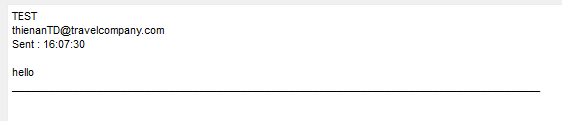
\includegraphics[width=16cm, height=5cm]{img/4.2.2d.png}
    \caption{Gửi email từ phòng du lịch nội địa đến phòng  hành chính thành công}
    \label{hinh422d}
\end{figure}



\subsubsection{FTP Server}
\begin{figure}[H]
    \centering
    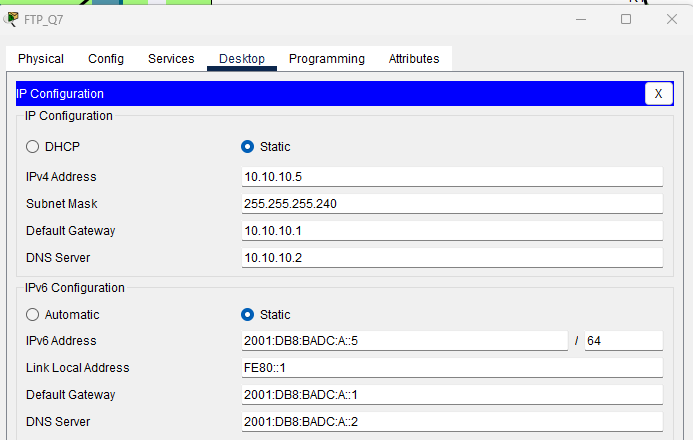
\includegraphics[width=16cm, height=14cm]{img/4.2.3a.png}
    \caption{Cấu hình Ipv4 và Ipv6 cho FTP Server}
    \label{hinh423a}
\end{figure}

\begin{figure}[H]
    \centering
    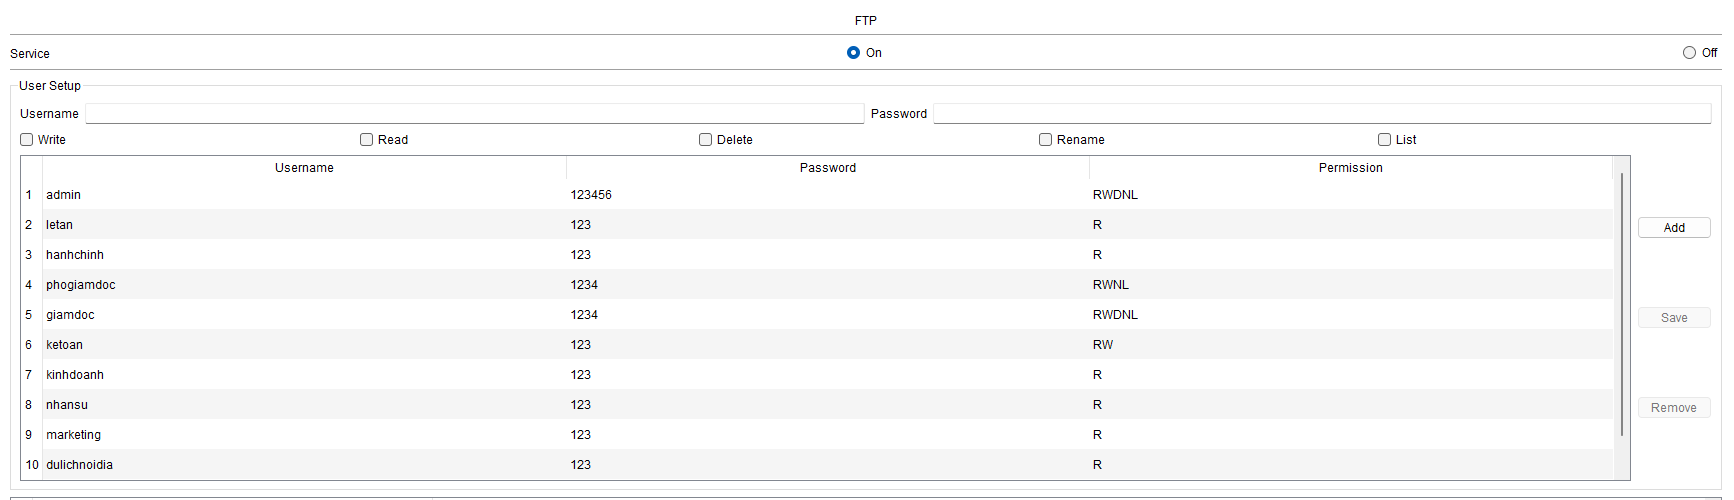
\includegraphics[width=16cm, height=8cm]{img/4.2.3b.png}
    \caption{ Bật dịch vụ FTP và tạo tài khoản cho các phòng chức năng}
    \label{hinh423b}
\end{figure}
\hspace*{0.25cm}Để kiểm tra chức năng FTP, ta sẽ tạo một file txt ở một máy của phòng kỹ thuật, sau đó gửi lên Server FTP. Để kiểm tra file vừa tạo có tồn tại ở ổ đĩa đó hay không, ta sẽ mở CMD nhập lệnh dir.\\
\begin{figure}[H]
    \centering
    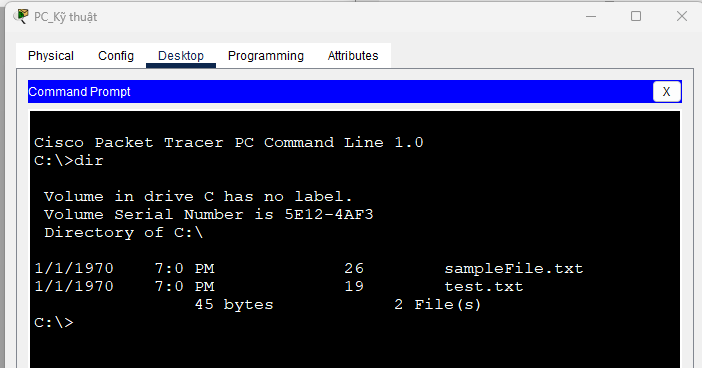
\includegraphics[width=16cm, height=8cm]{img/4.2.3c.png}
    \caption{File test.txt vừa tạo tồn tại trên ổ C của máy}
    \label{hinh423c}
\end{figure}
\hspace*{0.25cm}Khi xác định file có tồn tại trong máy, ta sẽ đăng nhập vào ftp và đưa file lên Server FTP bằng lệnh put [file].\\
\begin{figure}[H]
    \centering
    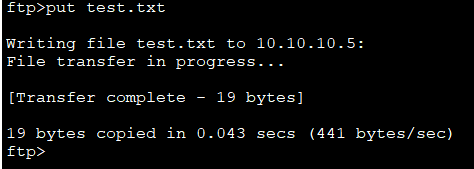
\includegraphics[width=12cm, height=6cm]{img/4.3.2d.png}
    \caption{Tải file lên server FTP}
    \label{hinh423d}
\end{figure}
\hspace*{0.25cm}Sau khi đã tải file thành công, các phòng chức năng khác có thể đăng nhập vào FTP để tải file về bằng câu lệnh get [file]\\
\begin{figure}[H]
    \centering
    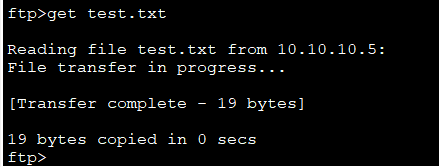
\includegraphics[width=12cm, height=6cm]{img/4.2.3e.png}
    \caption{Các phòng chức năng có thể tải file về máy}
    \label{hinh423e}
\end{figure}

\begin{figure}[H]
    \centering
    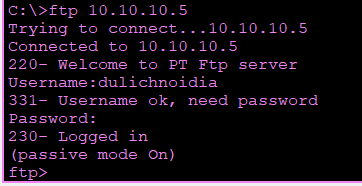
\includegraphics[width=12cm, height=6cm]{img/4.2.3f.png}
    \caption{Các phòng chức năng ở chi nhánh Thủ Đức cũng có thể đăng nhập vào ftp}
    \label{hinh423f}
\end{figure}

\subsubsection{RADIUS Server}
\begin{figure}[H]
    \centering
    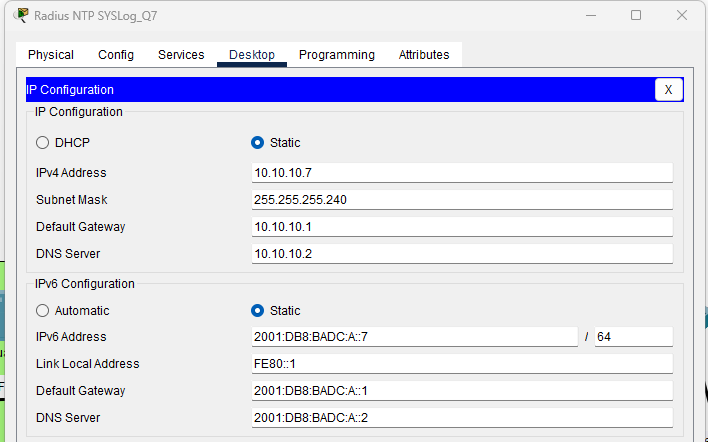
\includegraphics[width=16cm, height=14cm]{img/4.2.5a.png}
    \caption{Cấu hình Ipv4 và Ipv6 trên Server quận 7.}
    \label{hinh425a}
\end{figure}

\begin{figure}[H]
    \centering
    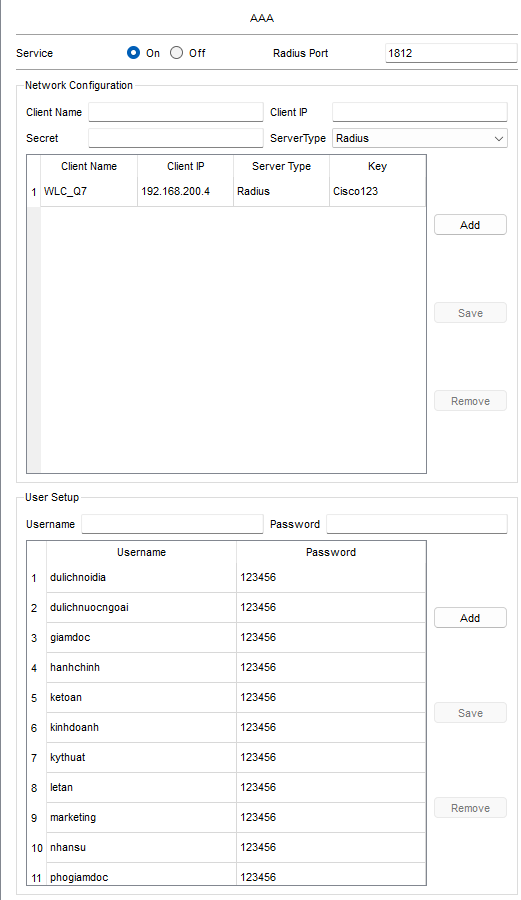
\includegraphics[width=16cm, height=20cm]{img/4.2.5b.png}
    \caption{Bật dịch vụ AAA và tạo các account cho các phòng chức năng}
    \label{hinh425b}
\end{figure}
\hspace*{0.25cm}Tương tự cấu hình tương tự ở Server Radius ở Thủ Đức\\
\begin{figure}[H]
    \centering
    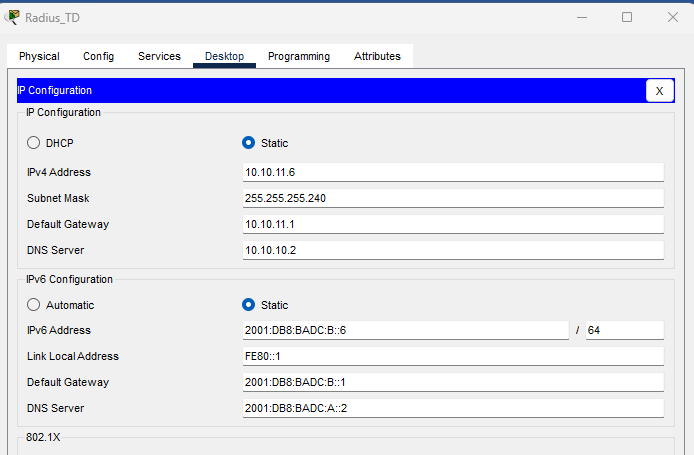
\includegraphics[width=16cm, height=14cm]{img/4.2.5c.png}
    \caption{Cấu hình Ipv4 và Ipv6 trên Server Thủ Đức}
    \label{hinh425c}
\end{figure}

\begin{figure}[H]
    \centering
    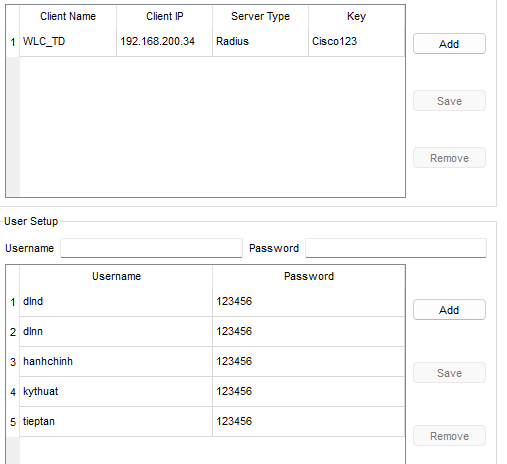
\includegraphics[width=16cm, height=16cm]{img/4.2.5d.png}
    \caption{Bật dịch vụ AAA và tạo các account cho các phòng chức năng}
    \label{hinh425d}
\end{figure}
\subsubsection{NTP Server}
\begin{figure}[H]
    \centering
    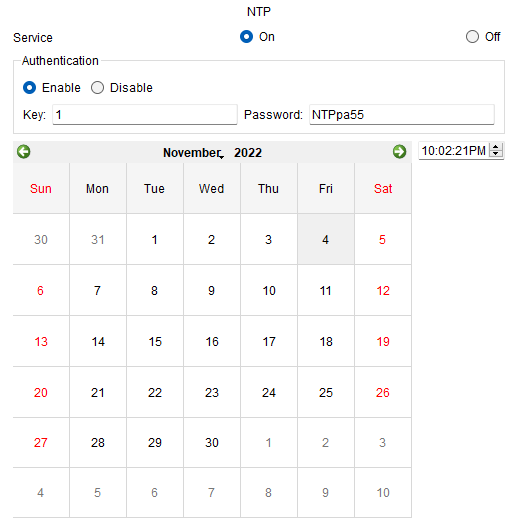
\includegraphics[width=16cm, height=14cm]{img/4.2.6.png}
    \caption{ Khởi động và cài đặt dịch vụ NTP.}
    \label{hinh426}
\end{figure}
\subsubsection{Syslog Server }
\begin{figure}[H]
    \centering
    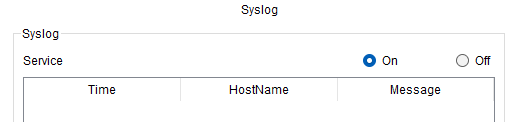
\includegraphics[width=16cm, height=6cm]{img/4.2.7.png}
    \caption{ Khởi động dịch vụ Syslog}
    \label{hinh427}
\end{figure}
\subsection{Cấu hình VLAN VÀ VTP}
\subsubsection{Khu vực Quận 7}
\hspace*{1cm}Chúng ta sẽ cấu hình các VLAN trên các Switch Layer 3, ở chi nhánh quận 7 sẽ có tổng cộng 13 VLAN, bao gồm: VLAN 10 cho phòng Lễ tân, 11 cho phòng Hành chính, 12 cho phòng Phó giám đốc, 13 cho phòng Giám đốc, 14 cho phòng Kế toán, 15 cho phòng Kinh doanh, 16 cho phòng Nhân sự, 17 cho phòng Kỹ thuật, 18 cho phòng Marketing, 19 cho phòng Du lịch nội địa, 20 cho phòng Du lịch nước ngoài, 110 cho WLC quản lý và 200 cho Khách hàng.\\
\hspace*{1cm}Tạo VLAN Database trên Switch Distribute 1 và 2:\\
\hspace*{2cm}\textit{vlan 10\\
\hspace*{2cm}name LETAN\\
\hspace*{2cm}vlan 11\\
\hspace*{2cm}name HANHCHINH\\
\hspace*{2cm}vlan 12\\
\hspace*{2cm}name PHOGIAMDOC\\
\hspace*{2cm}vlan 13\\
\hspace*{2cm}name GIAMDOC\\
\hspace*{2cm}vlan 14\\
\hspace*{2cm}name KETOAN\\
\hspace*{2cm}vlan 15\\
\hspace*{2cm}name KINHDOANH\\
\hspace*{2cm}vlan 16\\
\hspace*{2cm}name NHANSU\\
\hspace*{2cm}vlan 17\\
\hspace*{2cm}name KYTHUAT\\
\hspace*{2cm}vlan 18\\
\hspace*{2cm}name MARKETING\\
\hspace*{2cm}vlan 19\\
\hspace*{2cm}name DULICHNOIDIA\\
\hspace*{2cm}vlan 20\\
\hspace*{2cm}name DULICHNUOCNGOAI\\
\hspace*{2cm}vlan 200\\
\hspace*{2cm}name KHACHHANG\\
\hspace*{2cm}vlan 110\\
\hspace*{2cm}name WLC\_Q7\\}
\hspace*{1cm}Sau khi tạo các VLAN Database, ta sẽ cấu hình giao thức VTP cho các Switch, trong đó, Switch Distribute 1 sẽ là mode Server, Distribute 2 ở mode transparent. Switch Distribute 1 ở mode server sẽ dùng để tạo bản tin VTP, lắng nghe bản tin, thêm  xóa sửa VLAN. Switch Distribute 2 sẽ ở mode transparent để backup, dùng để thêm xóa sửa VLAN nhưng chỉ có tác dụng nội bộ trên switch cấu hình Transparent.
\renewcommand{\labelitemi}{$\blacksquare$}
\renewcommand\labelitemii{$\nabla$}
\renewcommand\labelitemiii{$\square$}
\begin{itemize}
  \item \textbf{Switch Distribution}
    \begin{itemize}
    \item Switch Distribute 1
    \begin{itemize}
      \item \textit{vtp domain dulichquan7.com\\
            vtp version 2\\
            vtp mode server\\
            vtp pass dulichquan7}
    \end{itemize}
    \item Switch Distribute 2
     \begin{itemize}
      \item \textit{vtp domain dulichquan7.com\\
                    vtp version 2\\
                    vtp mode transparent \\
                    vtp pass dulichquan7}  
    \end{itemize}
    \hspace*{0.25cm} Trunking các đường  Switch Distribute 1 và 2 nối với các Switch Access 
     \item Switch Distribute 1 và 2
     \begin{itemize}
      \item \textit{Interface range G1/0/1-9\\
                    switchport mode trunk}   
    \end{itemize}
   \end{itemize}
  \item \textbf{Switch Access}\\
\hspace*{1cm} Ở các Switch Access, nó sẽ ở mode client, có nhiệm vụ tạo và lắng nghe bản tin VTP\\
\hspace*{2cm}\textit{vtp domain dulichquan7.com\\
\hspace*{2cm}vtp version 2\\
\hspace*{2cm}vtp mode client\\
\hspace*{2cm}vtp pass dulichquan7\\} 
\hspace*{1cm}Các Switch Access nối với Switch Distribute 1 và 2 bằng các cổng Gigabit Ethernet 0/1 và 0/2, cho nên ta sẽ trunking các đường này.\\
\hspace*{2cm}\textit{Interface range G0/1-2\\
\hspace*{2cm}switchport mode trunk\\}
\hspace*{1cm}Đối với các port nối với các PC, ta sẽ gán port acces cho từng VLAN đã định sẵn
  \begin{itemize}
    \item \textbf{Switch Access Lễ Tân}
    \begin{itemize}
      \item \textit{interface f0/1\\
                    switchport mode access\\
                    switchport access vlan 10\\
                    interface f0/3\\
                    switchport mode trunk\\
                    switchport trunk native vlan 110\\}   
      
    \end{itemize}
    \item \textbf{Switch Access Tầng 2}
     \begin{itemize}
      \item \textit{interface f0/1\\
                    switchport mode access\\
                    switchport access vlan 13\\
                    interface f0/2\\
                    switchport mode access\\
                    switchport access vlan 11\\
                    interface f0/3\\
                    switchport mode access\\
                    switchport access vlan 12\\
                    interface f0/4\\
                    switchport mode trunk\\
                    switchport trunk native vlan 110\\
                    }
     
    \end{itemize}
     \item \textbf{Switch Access  Kế toán}
     \begin{itemize}
      \item \textit{interface f0/1\\
                    switchport mode access\\
                    switchport access vlan 14\\
                    interface f0/2\\
                    switchport mode trunk\\
                    switchport trunk native vlan 110\\}
     
    \end{itemize}
     \item \textbf{Switch Access  Kinh Doanh}
     \begin{itemize}
      \item \textit{interface f0/1\\
                    switchport mode access\\
                    switchport access vlan 15\\
                    interface f0/2\\
                    switchport mode trunk\\
                    switchport trunk native vlan 110\\}
     
    \end{itemize}
     \item \textbf{Switch Access  Nhân sự}
     \begin{itemize}
      \item \textit{interface f0/1\\
                    switchport mode access\\
                    switchport access vlan 16\\
                    interface f0/2\\
                    switchport mode trunk\\
                    switchport trunk native vlan 110\\}
     
    \end{itemize}
     \item \textbf{Switch Access  Kỹ thuật}
     \begin{itemize}
      \item \textit{interface f0/1\\
                    switchport mode access\\
                    switchport access vlan 17\\
                    interface f0/2\\
                    switchport mode trunk\\
                    switchport trunk native vlan 110\\
                    interface f0/3\\
                    switchport mode trunk\\
                    switchport trunk native vlan 110\\
                    interface FastEthernet0/4\\
                    switchport mode access\\
                     switchport access vlan 17\\}
     
    \end{itemize}
     \item \textbf{Switch Access  Marketing}
     \begin{itemize}
      \item \textit{interface f0/1\\
                    switchport mode access\\
                    switchport access vlan 18\\
                    interface f0/2\\
                    switchport mode trunk\\
                    switchport trunk native vlan 110\\}
     
    \end{itemize}
     \item \textbf{Switch Access  Du lịch nội địa}
     \begin{itemize}
      \item \textit{interface f0/1\\
                    switchport mode access\\
                    switchport access vlan 19\\
                    interface f0/2\\
                    switchport mode trunk\\
                    switchport trunk native vlan 110\\}
     
    \end{itemize}
     \item \textbf{witch Access  Du lịch nước ngoài}
     \begin{itemize}
      \item \textit{interface f0/1\\
                    switchport mode access\\
                    switchport access vlan 20\\
                    interface f0/3\\
                    switchport mode trunk\\
                    switchport trunk native vlan 110\\}
     
    \end{itemize}
   \end{itemize}
\end{itemize}
\subsubsection{Khu vực Thủ Đức}
\hspace*{1cm}Chúng ta sẽ cấu hình các VLAN trên các Switch Layer 3, ở chi nhánh Thủ Đức sẽ có tổng cộng 7 VLAN, bao gồm : VLAN 21 cho phòng Tiếp Tân, 22 cho phòng Du lịch nội địa , 23 cho phòng Du lịch nước ngoài, 24 cho phòng Kỹ thuật, 25 cho phòng Hành chính, 111 cho WLC quản lý và 100 cho Khách hàng.\\
\hspace*{1cm}Tạo VLAN Database trên Switch Distribute 1 và 2:\\
\hspace*{2cm}\textit{vlan 21\\
              \hspace*{2cm} name TIEPTAN\\
              \hspace*{2cm}  vlan 22\\
              \hspace*{2cm}  name DULICHNOIDIA\_TD\\
              \hspace*{2cm}    vlan 23\\
              \hspace*{2cm}    name DULICHNUOCNGOAI\_TD\\
              \hspace*{2cm}     vlan 24\\
              \hspace*{2cm}     name KYTHUAT\_TD\\
              \hspace*{2cm}     vlan 25\\
              \hspace*{2cm}     name HANHCHINH\_TD\\
              \hspace*{2cm}    vlan 111\\
              \hspace*{2cm}     name WLC\_TD\\
              \hspace*{2cm}      vlan 100\\
              \hspace*{2cm}    name KHACHHANG\_TD\\}
\hspace*{1cm}Sau khi tạo các VLAN Database, ta sẽ cấu hình giao thức VTP cho các Switch, tương tự như khu vực Quận 7.
\renewcommand{\labelitemi}{$\blacksquare$}
\renewcommand\labelitemii{$\nabla$}
\renewcommand\labelitemiii{$\square$}
\begin{itemize}
  \item \textbf{Switch Distribution}
    \begin{itemize}
    \item Switch Distribute 1
    \begin{itemize}
      \item \textit{vtp domain dulichthuduc.com\\
                    vtp version 2\\
                    vtp mode server\\
                    vtp pass dulichthuduc}
    \end{itemize}
    \item Switch Distribute 2
     \begin{itemize}
      \item \textit{vtp domain dulichthuduc.com\\
                    vtp version 2\\
                    vtp mode transparent \\
                    vtp pass dulichthuduc}  
    \end{itemize}
    \hspace*{1cm} Trunking các đường  Switch Distribute 1 và 2 nối với các Switch Access  \\
     \item Switch Distribute 1 và 2
     \begin{itemize}
      \item \textit{Interface range G1/0/1-5\\
                    switchport mode trunk}   
    \end{itemize}
   \end{itemize}
  \item \textbf{Switch Access}\\
\hspace*{1cm} Ở các Switch Access, nó sẽ ở mode client, có nhiệm vụ tạo và lắng nghe bản tin VTP\\
\hspace*{2cm}\textit{vtp domain dulichthuduc.com\\
 \hspace*{2cm}  vtp version 2\\
 \hspace*{2cm}  vtp mode client\\
 \hspace*{2cm}  vtp pass dulichthuduc\\} 
\hspace*{1cm}Các Switch Access nối với Switch Distribute 1 và 2 bằng các cổng Gigabit Ethernet 0/1 và 0/2, cho nên ta sẽ trunking các đường này.\\
\hspace*{2cm}\textit{Interface range G0/1-2\\
\hspace*{2cm}switchport mode trunk\\}
\hspace*{1cm}Đối với các port nối với các PC, ta sẽ gán port acces cho từng VLAN đã định sẵn
  \begin{itemize}
    \item \textbf{Switch Access Tiếp Tân}
    \begin{itemize}
      \item \textit{switchport mode trunk\\
                    interface f0/1\\
                    switchport mode access\\
                    switchport access vlan 21\\
                    interface f0/2\\
                    switchport mode trunk\\
                    switchport trunk native vlan 111}   
      
    \end{itemize}
   
     \item \textbf{Switch Access  Du lịch nội địa}
     \begin{itemize}
      \item \textit{interface f0/1\\
                    switchport mode access\\
                    switchport access vlan 22\\
                    interface f0/2\\
                    switchport mode trunk\\
                    switchport trunk native vlan 111}
     
    \end{itemize}
     \item \textbf{witch Access  Du lịch nước ngoài}
     \begin{itemize}
      \item \textit{interface f0/1\\
                    switchport mode access\\
                    switchport access vlan 23\\
                    interface f0/2\\
                    switchport mode trunk\\
                    switchport trunk native vlan 111\\}
     
    \end{itemize}
     \item \textbf{Switch Access Kỹ thuật}
     \begin{itemize}
      \item \textit{interface f0/1\\
                    switchport mode access\\
                    switchport access vlan 24\\
                    interface f0/2\\
                    switchport mode trunk\\
                    switchport trunk native vlan 111\\
                    interface f0/3\\
                    switchport mode trunk\\
                    switchport trunk native vlan 111\\
                    interface FastEthernet0/4\\
                    switchport mode access\\
                     switchport access vlan 24}
     
    \end{itemize}
     \item \textbf{Switch Access Hành chính}
     \begin{itemize}
      \item \textit{interface f0/1\\
                    switchport mode access\\
                    switchport access vlan 25\\
                    interface f0/2\\
                    switchport mode trunk\\
                    switchport trunk native vlan 111}
                         
    \end{itemize}
   \end{itemize}
\end{itemize}
\subsection{Cấu hình WLC và Light Access Point }
\begin{figure}[H]
    \centering
    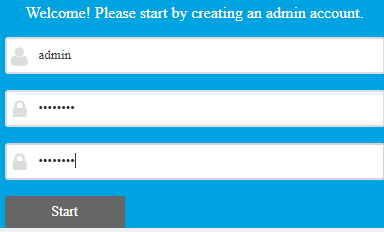
\includegraphics[width=12cm, height=6cm]{img/4.6a.png}
    \caption{Tạo tài khoản }
    \label{hinh46a}
\end{figure}
\hspace*{1cm}Truy cập vào địa chỉ IP đã đặt trên WLC để tạo tài khoản đăng nhập, sau đó tiến hành tạo các Interface và WLAN phù hợp. Sau khi tạo xong, chọn apply để tạo.\\
\begin{figure}[H]
    \centering
    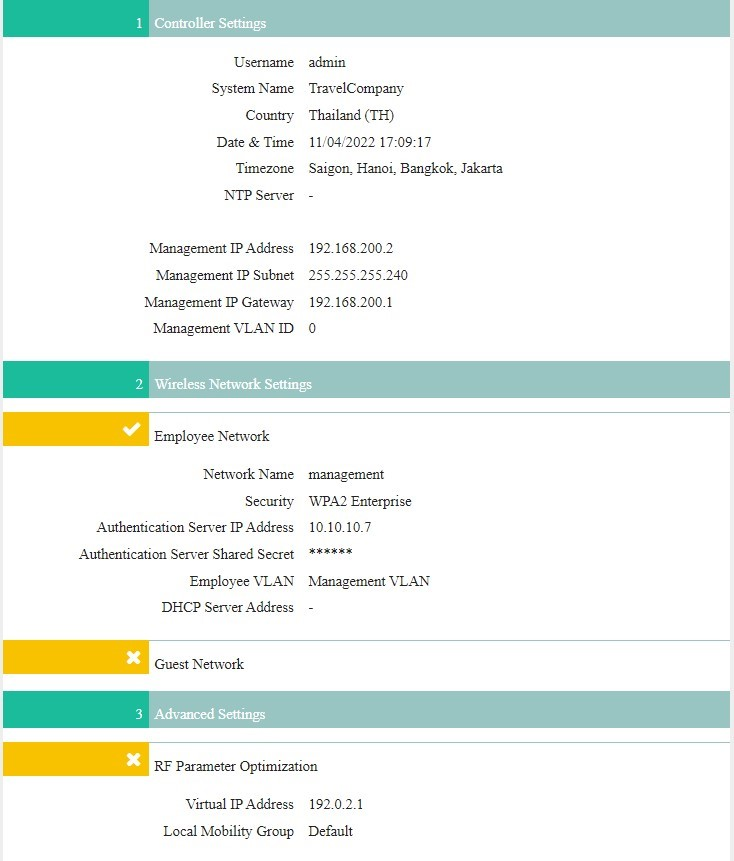
\includegraphics[width=16cm, height=18cm]{img/4.6b.jpg}
    \caption{Thông tin sau khi tạo }
    \label{hinh46b}
\end{figure}
\hspace*{1cm}Sau khi tạo tài khoản, truy cập địa chỉ: https://192.168.200.4 để đăng nhập vào giao diện WLC. Đăng nhập với tài khoản admin và mật khẩu Cisco123. Sau khi hiển thị giao diện WLC, chúng ta sẽ tiến hành tạo các Interface và các WLAN ID.\\
\begin{figure}[H]
    \centering
    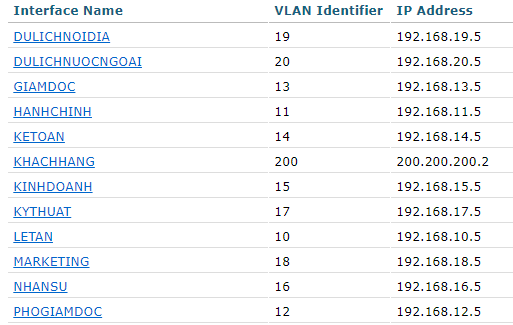
\includegraphics[width=16cm, height=14cm]{img/4.6c.png}
    \caption{Tạo Interface cho các WLAN}
    \label{hinh46c}
\end{figure}

\begin{figure}[H]
    \centering
    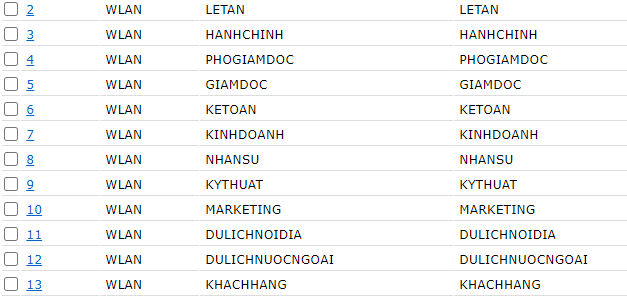
\includegraphics[width=16cm, height=10cm]{img/4.6d.png}
    \caption{Tạo WLAN ID }
    \label{hinh46d}
\end{figure}
\hspace*{1cm}Tạo WLAN, ở Layer 2 Security , chọn WPA +WPA2 với thông số mã hóa WPA2 là AES và khóa xác thực là 802.1X. Sau đó, ở phần cấu hình AAA, chọn Server Radius với số port khớp với Server mà chúng ta đã tạo ở hệ thống.\\
\begin{figure}[H]
    \centering
    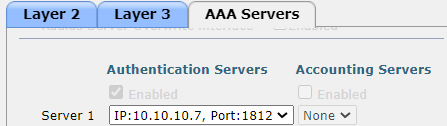
\includegraphics[width=12cm, height=6cm]{img/4.6e.png}
    \caption{Chọn dải IP Radius phù hợp}
    \label{hinh46e}
\end{figure}
\hspace*{1cm}Ở phần Flex Connect, chúng ta sẽ chọn hai thông số là Flex Connect Switching và Local Auth để tạo đường hầm CAPWAP đến WLC, một là để quản lý, còn lại là lưu lượng dữ liệu.\\
\hspace*{1cm}Sau khi đã tạo các WLAN và các Light Access Point đã kết nối được, lúc này chúng ta sẽ chia các Light Access Point ở các tầng để phát cố định các Wifi cần thiết. Ở tầng 1, chúng ta sẽ cho LAP chỉ phát một wifi cho phòng lễ tân, còn ở tầng 2, LAP sẽ phát wifi cho ba phòng hành chính, phó giám đốc và giám đốc, 3 tầng còn lại mỗi LAP sẽ phát wifi cho các phòng chức năng tương ứng.\\
\begin{figure}[H]
    \centering
    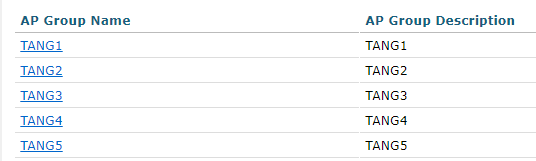
\includegraphics[width=16cm, height=6cm]{img/4.6f.png}
    \caption{Tạo AP Group}
    \label{hinh46f}
\end{figure}
\begin{figure}[H]
    \centering
    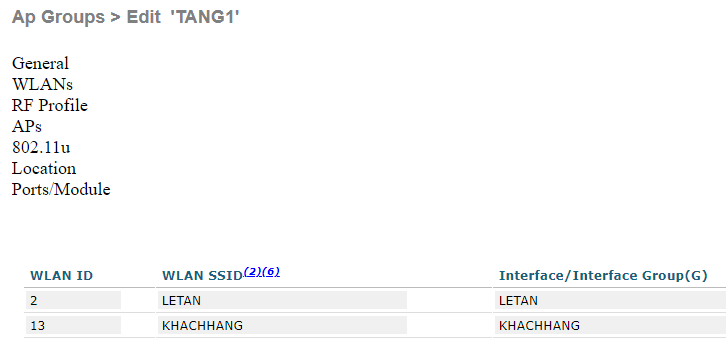
\includegraphics[width=16cm, height=10cm]{img/4.6g.png}
    \caption{Cấu hình các LAP phát Wifi cho WLAN }
    \label{hinh46g}
\end{figure}
\hspace*{0.25cm} Sau khi đã cấu hình xong , vào các PC tạo profile để kết nối.
\begin{figure}[H]
    \centering
    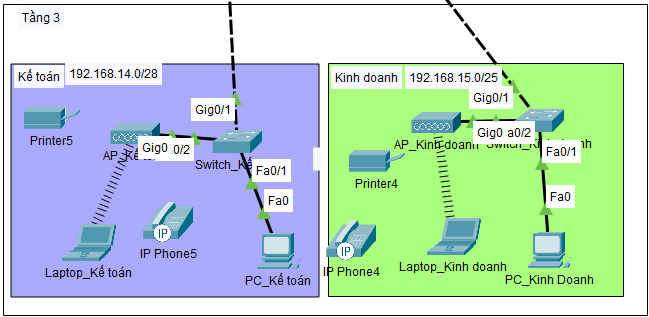
\includegraphics[width=16cm, height=10cm]{img/4.6h.png}
    \caption{Các PC kết nối wifi thành công }
    \label{hinh46h}
\end{figure}
\hspace*{0.25cm}Cấu hình tương tự ở chi nhánh Thủ Đức.
\subsection{Cấu hình DHCPv4 và DHCPv6}
\subsubsection{Khu vực Quận 7}
\hspace*{0.25cm}Tạo các pool DHCP cho các VLAN, bao gồm ipv4 và ipv6. Cấu hình của chức năng này sẽ được cấu hình trên DHCP server, cấp phát các IP động xuống cho các VLAN.\\
\begin{figure}[H]
    \centering
    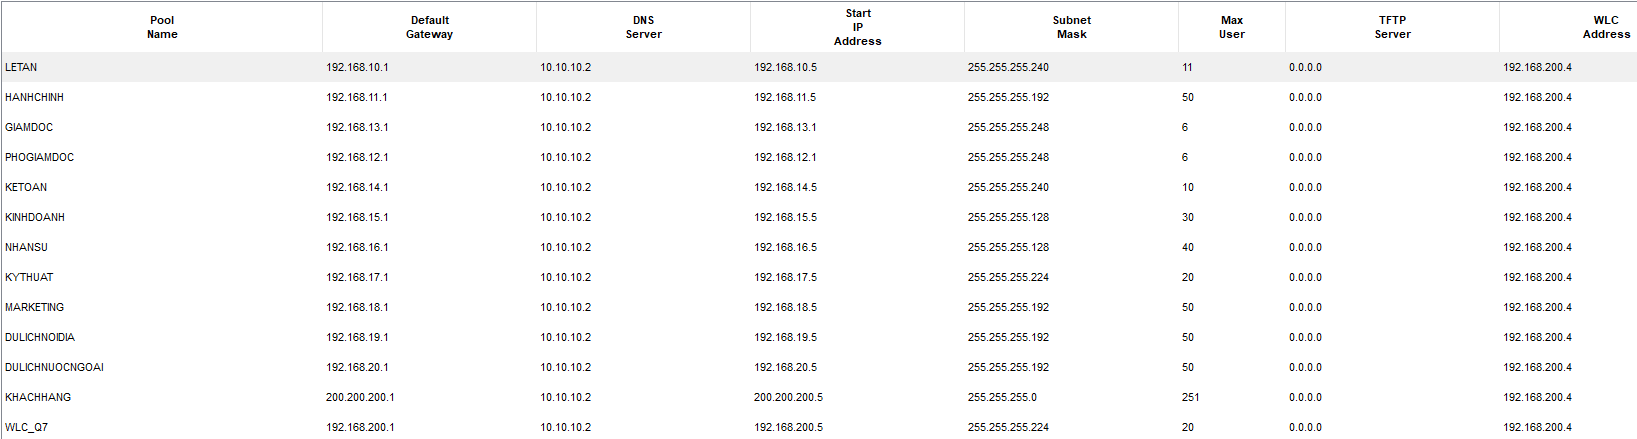
\includegraphics[width=16cm, height=8cm]{img/471.png}
    \caption{Tạo các Pool DHCP trên Server}
    \label{hinh471}
\end{figure}
\hspace*{0.25cm}Sau khi tạo pool trên Server, cấu hình inter-vlan trên hai switch Distribution như sau\\
\hspace*{1cm}\textbf{Switch Distribution 1}\\
\hspace*{2cm}\textit{int vlan 10\\
\hspace*{2cm}ip add 192.168.10.3 255.255.255.240\\
\hspace*{2cm}ipv6 add 2001:db8:acad:a::3/64\\
\hspace*{2cm}ip help 10.10.10.6\\
\hspace*{2cm}int vlan 11\\
\hspace*{2cm}ip add 192.168.11.3 255.255.255.192\\
\hspace*{2cm}ipv6 add 2001:db8:acad:b::3/64\\
\hspace*{2cm}ip help 10.10.10.6\\
\hspace*{2cm}int vlan 12\\
\hspace*{2cm}ip add 192.168.12.3 255.255.255.248\\
\hspace*{2cm}ipv6 add 2001:db8:acad:c::3/64\\
\hspace*{2cm}ip help 10.10.10.6\\
\hspace*{2cm}int vlan 13\\
\hspace*{2cm}ip add 192.168.13.3 255.255.255.248\\
\hspace*{2cm}ipv6 add 2001:db8:acad:d::3/64\\
\hspace*{2cm}ip help 10.10.10.6\\
\hspace*{2cm}int vlan 14\\
\hspace*{2cm}ip add 192.168.14.3 255.255.255.240\\
\hspace*{2cm}ipv6 add 2001:db8:acad:e::3/64\\
\hspace*{2cm}ip help 10.10.10.6\\
\hspace*{2cm}int vlan 15\\
\hspace*{2cm}ip add 192.168.15.3 255.255.255.128\\
\hspace*{2cm}ipv6 add 2001:db8:acad:f::3/64\\
\hspace*{2cm}ip help 10.10.10.6\\
\hspace*{2cm}int vlan 16\\
\hspace*{2cm}ip add 192.168.16.3 255.255.255.128\\
\hspace*{2cm}ipv6 add 2001:db8:acad:16::3/64\\
\hspace*{2cm}ip help 10.10.10.6\\
\hspace*{2cm}int vlan 17\\
\hspace*{2cm}ip add 192.168.17.3 255.255.255.224\\
\hspace*{2cm}ipv6 add 2001:db8:acad:17::3/64\\
\hspace*{2cm}ip help 10.10.10.6\\
\hspace*{2cm}int vlan 18\\
\hspace*{2cm}ip add 192.168.18.3 255.255.255.192\\
\hspace*{2cm}ipv6 add 2001:db8:acad:18::3/64\\
\hspace*{2cm}ip help 10.10.10.6\\
\hspace*{2cm}int vlan 19\\
\hspace*{2cm}ip add 192.168.19.3 255.255.255.192\\
\hspace*{2cm}ipv6 add 2001:db8:acad:19::3/64\\
\hspace*{2cm}ip help 10.10.10.6\\
\hspace*{2cm}int vlan 20\\
\hspace*{2cm}ip add 192.168.20.3 255.255.255.192\\
\hspace*{2cm}ipv6 add 2001:db8:acad:20::3/64\\
\hspace*{2cm}ip help 10.10.10.6\\
\hspace*{2cm}int vlan 200\\
\hspace*{2cm}ip add 200.200.200.3 255.255.255.0\\
\hspace*{2cm}ipv6 add 2001:db8:acad:200::3/64\\
\hspace*{2cm}ip help 10.10.10.6\\
\hspace*{2cm}int vlan 110\\
\hspace*{2cm}ip add 192.168.200.3 255.255.255.224\\
\hspace*{2cm}ipv6 add 2001:db8:acad:110::3/64\\
\hspace*{2cm}ip help 10.10.10.6\\
}

\hspace*{1cm}\textbf{Switch Distribution 2}\\
\hspace*{2cm}\textit{int vlan 10\\
\hspace*{2cm}ip add 192.168.10.2 255.255.255.240\\
\hspace*{2cm}ipv6 add 2001:db8:acad:a::2/64\\
\hspace*{2cm}ip help 10.10.10.6\\
\hspace*{2cm}int vlan 11\\
\hspace*{2cm}ip add 192.168.11.2 255.255.255.192\\
\hspace*{2cm}ipv6 add 2001:db8:acad:b::2/64\\
\hspace*{2cm}ip help 10.10.10.6\\
\hspace*{2cm}int vlan 12\\
\hspace*{2cm}ip add 192.168.12.2 255.255.255.248\\
\hspace*{2cm}ipv6 add 2001:db8:acad:c::2/64\\
\hspace*{2cm}ip help 10.10.10.6\\
\hspace*{2cm}int vlan 13\\
\hspace*{2cm}ip add 192.168.13.2 255.255.255.248\\
\hspace*{2cm}ipv6 add 2001:db8:acad:d::2/64\\
\hspace*{2cm}ip help 10.10.10.6\\
\hspace*{2cm}int vlan 14\\
\hspace*{2cm}ip add 192.168.14.2 255.255.255.240\\
\hspace*{2cm}ipv6 add 2001:db8:acad:e::2/64\\
\hspace*{2cm}ip help 10.10.10.6\\
\hspace*{2cm}int vlan 15\\
\hspace*{2cm}ip add 192.168.15.2 255.255.255.128\\
\hspace*{2cm}ipv6 add 2001:db8:acad:f::2/64\\
\hspace*{2cm}ip help 10.10.10.6\\
\hspace*{2cm}int vlan 16\\
\hspace*{2cm}ip add 192.168.16.2 255.255.255.128\\
\hspace*{2cm}ipv6 add 2001:db8:acad:16::2/64\\
\hspace*{2cm}ip help 10.10.10.6\\
\hspace*{2cm}int vlan 17\\
\hspace*{2cm}ip add 192.168.17.2 255.255.255.224\\
\hspace*{2cm}ipv6 add 2001:db8:acad:17::2/64\\
\hspace*{2cm}ip help 10.10.10.6\\
\hspace*{2cm}int vlan 18\\
\hspace*{2cm}ip add 192.168.18.2 255.255.255.192\\
\hspace*{2cm}ipv6 add 2001:db8:acad:18::2/64\\
\hspace*{2cm}ip help 10.10.10.6\\
\hspace*{2cm}int vlan 19\\
\hspace*{2cm}ip add 192.168.19.2 255.255.255.192\\
\hspace*{2cm}ipv6 add 2001:db8:acad:19::2/64\\
\hspace*{2cm}ip help 10.10.10.6\\
\hspace*{2cm}int vlan 20\\
\hspace*{2cm}ip add 192.168.20.2 255.255.255.192\\
\hspace*{2cm}ipv6 add 2001:db8:acad:20::2/64\\
\hspace*{2cm}ip help 10.10.10.6\\
\hspace*{2cm}int vlan 200\\
\hspace*{2cm}ip add 200.200.200.2 255.255.255.0\\
\hspace*{2cm}ipv6 add 2001:db8:acad:200::2/64\\
\hspace*{2cm}ip help 10.10.10.6\\
\hspace*{2cm}int vlan 110\\
\hspace*{2cm}ip add 192.168.200.2 255.255.255.224\\
\hspace*{2cm}ipv6 add 2001:db8:acad:110::2/64\\
\hspace*{2cm}ip help 10.10.10.6\\}
\subsubsection{Khu vực Thủ Đức}
\hspace*{0.25cm}Tạo các pool DHCP cho các VLAN tương tự khu vực quận 7\\
\begin{figure}[H]
    \centering
    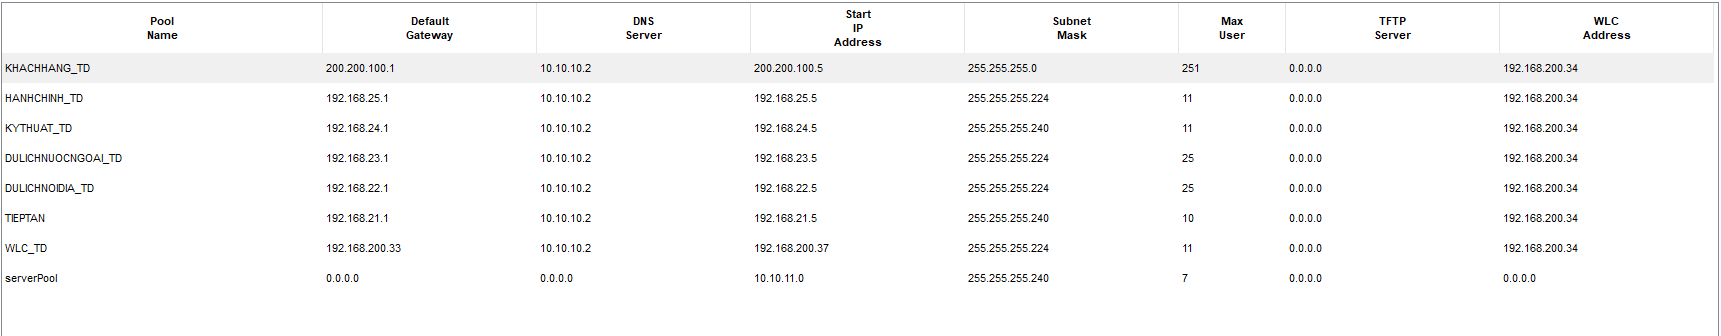
\includegraphics[width=16cm, height=8cm]{img/472.png}
    \caption{Tạo các Pool DHCP trên Server}
    \label{hinh472}
\end{figure}
\hspace*{0.25cm}Sau khi tạo pool trên Server, cấu hình inter-vlan trên hai switch Distribution như sau\\
\hspace*{1cm}\textbf{Switch Distribution 1}\\
\hspace*{2cm}\textit{int vlan 21\\
\hspace*{2cm}ip add 192.168.21.3 255.255.255.240\\
\hspace*{2cm}ipv6 add 2001:db8:acad:21::3/64\\
\hspace*{2cm}ip help 10.10.11.5\\
\hspace*{2cm}int vlan 22\\
\hspace*{2cm}ip add 192.168.22.3 255.255.255.224\\
\hspace*{2cm}ipv6 add 2001:db8:acad:22::3/64\\
\hspace*{2cm}ip help 10.10.11.5\\
\hspace*{2cm}int vlan 23\\
\hspace*{2cm}ip add 192.168.23.3 255.255.255.224\\
\hspace*{2cm}ipv6 add 2001:db8:acad:23::3/64\\
\hspace*{2cm}ip help 10.10.11.5\\
\hspace*{2cm}int vlan 24\\
\hspace*{2cm}ip add 192.168.24.3 255.255.255.240\\
\hspace*{2cm}ipv6 add 2001:db8:acad:24::3/64\\
\hspace*{2cm}ip help 10.10.11.5\\
\hspace*{2cm}int vlan 25\\
\hspace*{2cm}ip add 192.168.25.3 255.255.255.224\\
\hspace*{2cm}ipv6 add 2001:db8:acad:25::3/64\\
\hspace*{2cm}ip help 10.10.11.5\\
\hspace*{2cm}int vlan 100\\
\hspace*{2cm}ip add 200.200.100.3 255.255.255.0\\
\hspace*{2cm}ipv6 add 2001:db8:acad:100::3/64\\
\hspace*{2cm}ip help 10.10.11.5\\
\hspace*{2cm}int vlan 111\\
\hspace*{2cm}ip add 192.168.200.36 255.255.255.224\\
\hspace*{2cm}ipv6 add 2001:db8:acad:111::3/64\\
\hspace*{2cm}ip help 10.10.11.5\\}
\hspace*{1cm}\textbf{Switch Distribution 2}\\
\hspace*{2cm}\textit{int vlan 21\\
\hspace*{2cm}ip add 192.168.21.2 255.255.255.240\\
\hspace*{2cm}ipv6 add 2001:db8:acad:21::2/64\\
\hspace*{2cm}ip help 10.10.11.5\\
\hspace*{2cm}int vlan 22\\
\hspace*{2cm}ip add 192.168.22.2 255.255.255.224\\
\hspace*{2cm}ipv6 add 2001:db8:acad:22::2/64\\
\hspace*{2cm}ip help 10.10.11.5\\
\hspace*{2cm}int vlan 23\\
\hspace*{2cm}ip add 192.168.23.2 255.255.255.224\\
\hspace*{2cm}ipv6 add 2001:db8:acad:23::2/64\\
\hspace*{2cm}ip help 10.10.11.5\\
\hspace*{2cm}int vlan 24\\
\hspace*{2cm}ip add 192.168.24.2 255.255.255.240\\
\hspace*{2cm}ipv6 add 2001:db8:acad:24::2/64\\
\hspace*{2cm}ip help 10.10.11.5\\
\hspace*{2cm}int vlan 25\\
\hspace*{2cm}ip add 192.168.25.2 255.255.255.224\\
\hspace*{2cm}ipv6 add 2001:db8:acad:25::2/64\\
\hspace*{2cm}ip help 10.10.11.5\\
\hspace*{2cm}int vlan 100\\
\hspace*{2cm}ip add 200.200.100.2 255.255.255.0\\
\hspace*{2cm}ipv6 add 2001:db8:acad:100::200/64\\
\hspace*{2cm}ip help 10.10.11.5\\
\hspace*{2cm}int vlan 111\\
\hspace*{2cm}ip add 192.168.200.35 255.255.255.224\\
\hspace*{2cm}ipv6 add 2001:db8:acad:111::2/64\\
\hspace*{2cm}ip help 10.10.11.5\\}
\subsection{Cấu hình DHCP Snooping}
\subsubsection{Khu vực Quận 7}
\hspace*{0.25cm}Để chống giả mạo DHCP Server, ngăn chặn những cuộc tấn công của tin tặc vào hệ thống mạng và đánh cắp các thông tin quan trọng của doanh nghiệp, chúng ta sẽ sử dụng DHCP Snooping, khi đó máy tính sẽ được bảo vệ và ngăn chặn khỏi các cuộc tấn công này.\\
\hspace*{1cm}\textbf{Switch Access Lễ Tân}\\
\hspace*{2cm}\textit{no ip dhcp snooping information option\\
\hspace*{2cm}ip dhcp snooping vlan 10\\
\hspace*{2cm}ip dhcp snooping vlan 11\\
\hspace*{2cm}ip dhcp snooping vlan 12\\
\hspace*{2cm}ip dhcp snooping vlan 13\\
\hspace*{2cm}ip dhcp snooping vlan 14\\
\hspace*{2cm}ip dhcp snooping vlan 15\\
\hspace*{2cm}ip dhcp snooping vlan 16\\
\hspace*{2cm}ip dhcp snooping vlan 17\\
\hspace*{2cm}ip dhcp snooping vlan 18\\
\hspace*{2cm}ip dhcp snooping vlan 19\\
\hspace*{2cm}ip dhcp snooping vlan 20\\
\hspace*{2cm}ip dhcp snooping vlan 110\\
\hspace*{2cm}ip dhcp snooping vlan 200\\
\hspace*{2cm}inter range g0/1-2\\
\hspace*{2cm}ip dhcp snooping trust\\
\hspace*{2cm}ex\\
\hspace*{2cm}inter range f0/1-3\\
\hspace*{2cm}ip dhcp snooping limit rate 30\\}
\hspace*{1cm}\textbf{Switch Access Tầng 2}\\
\hspace*{2cm}\textit{no ip dhcp snooping information option\\
\hspace*{2cm}ip dhcp snooping vlan 10\\
\hspace*{2cm}ip dhcp snooping vlan 11\\
\hspace*{2cm}ip dhcp snooping vlan 12\\
\hspace*{2cm}ip dhcp snooping vlan 13\\
\hspace*{2cm}ip dhcp snooping vlan 14\\
\hspace*{2cm}ip dhcp snooping vlan 15\\
\hspace*{2cm}ip dhcp snooping vlan 16\\
\hspace*{2cm}ip dhcp snooping vlan 17\\
\hspace*{2cm}ip dhcp snooping vlan 18\\
\hspace*{2cm}ip dhcp snooping vlan 19\\
\hspace*{2cm}ip dhcp snooping vlan 20\\
\hspace*{2cm}ip dhcp snooping vlan 110\\
\hspace*{2cm}ip dhcp snooping vlan 200\\
\hspace*{2cm}inter range g0/1-2\\
\hspace*{2cm}ip dhcp snooping trust\\
\hspace*{2cm}ex\\
\hspace*{2cm}inter range f0/1-4\\
\hspace*{2cm}ip dhcp snooping limit rate 30\\}
\hspace*{1cm}\textbf{Switch Access Kế toán}\\
\hspace*{2cm}\textit{no ip dhcp snooping information option\\
\hspace*{2cm}ip dhcp snooping vlan 10\\
\hspace*{2cm}ip dhcp snooping vlan 11\\
\hspace*{2cm}ip dhcp snooping vlan 12\\
\hspace*{2cm}ip dhcp snooping vlan 13\\
\hspace*{2cm}ip dhcp snooping vlan 14\\
\hspace*{2cm}ip dhcp snooping vlan 15\\
\hspace*{2cm}ip dhcp snooping vlan 16\\
\hspace*{2cm}ip dhcp snooping vlan 17\\
\hspace*{2cm}ip dhcp snooping vlan 18\\
\hspace*{2cm}ip dhcp snooping vlan 19\\
\hspace*{2cm}ip dhcp snooping vlan 20\\
\hspace*{2cm}ip dhcp snooping vlan 110\\
\hspace*{2cm}ip dhcp snooping vlan 200\\
\hspace*{2cm}inter range g0/1-2\\
\hspace*{2cm}ip dhcp snooping trust\\
\hspace*{2cm}ex\\
\hspace*{2cm}inter range f0/1-2\\
\hspace*{2cm}ip dhcp snooping limit rate 30\\}
\hspace*{1cm}\textbf{Switch Access Kinh Doanh}\\
\hspace*{2cm}\textit{no ip dhcp snooping information option\\
\hspace*{2cm}ip dhcp snooping vlan 10\\
\hspace*{2cm}ip dhcp snooping vlan 11\\
\hspace*{2cm}ip dhcp snooping vlan 12\\
\hspace*{2cm}ip dhcp snooping vlan 13\\
\hspace*{2cm}ip dhcp snooping vlan 14\\
\hspace*{2cm}ip dhcp snooping vlan 15\\
\hspace*{2cm}ip dhcp snooping vlan 16\\
\hspace*{2cm}ip dhcp snooping vlan 17\\
\hspace*{2cm}ip dhcp snooping vlan 18\\
\hspace*{2cm}ip dhcp snooping vlan 19\\
\hspace*{2cm}ip dhcp snooping vlan 20\\
\hspace*{2cm}ip dhcp snooping vlan 110\\
\hspace*{2cm}ip dhcp snooping vlan 200\\
\hspace*{2cm}inter range g0/1-2\\
\hspace*{2cm}ip dhcp snooping trust\\
\hspace*{2cm}ex\\
\hspace*{2cm}inter range f0/1-2\\
\hspace*{2cm}ip dhcp snooping limit rate 30\\}
\hspace*{1cm}\textbf{Switch Access Nhân sự}\\
\hspace*{2cm}\textit{no ip dhcp snooping information option\\
\hspace*{2cm}ip dhcp snooping vlan 10\\
\hspace*{2cm}ip dhcp snooping vlan 11\\
\hspace*{2cm}ip dhcp snooping vlan 12\\
\hspace*{2cm}ip dhcp snooping vlan 13\\
\hspace*{2cm}ip dhcp snooping vlan 14\\
\hspace*{2cm}ip dhcp snooping vlan 15\\
\hspace*{2cm}ip dhcp snooping vlan 16\\
\hspace*{2cm}ip dhcp snooping vlan 17\\
\hspace*{2cm}ip dhcp snooping vlan 18\\
\hspace*{2cm}ip dhcp snooping vlan 19\\
\hspace*{2cm}ip dhcp snooping vlan 20\\
\hspace*{2cm}ip dhcp snooping vlan 110\\
\hspace*{2cm}ip dhcp snooping vlan 200\\
\hspace*{2cm}inter range g0/1-2\\
\hspace*{2cm}ip dhcp snooping trust\\
\hspace*{2cm}ex\\
\hspace*{2cm}inter range f0/1-2\\
\hspace*{2cm}ip dhcp snooping limit rate 30\\}
\hspace*{1cm}\textbf{Switch Access Kỹ Thuật}\\
\hspace*{2cm}\textit{no ip dhcp snooping information option\\
\hspace*{2cm}ip dhcp snooping vlan 10\\
\hspace*{2cm}ip dhcp snooping vlan 11\\
\hspace*{2cm}ip dhcp snooping vlan 12\\
\hspace*{2cm}ip dhcp snooping vlan 13\\
\hspace*{2cm}ip dhcp snooping vlan 14\\
\hspace*{2cm}ip dhcp snooping vlan 15\\
\hspace*{2cm}ip dhcp snooping vlan 16\\
\hspace*{2cm}ip dhcp snooping vlan 17\\
\hspace*{2cm}ip dhcp snooping vlan 18\\
\hspace*{2cm}ip dhcp snooping vlan 19\\
\hspace*{2cm}ip dhcp snooping vlan 20\\
\hspace*{2cm}ip dhcp snooping vlan 110\\
\hspace*{2cm}ip dhcp snooping vlan 200\\
\hspace*{2cm}inter range g0/1-2\\
\hspace*{2cm}ip dhcp snooping trust\\
\hspace*{2cm}ex\\
\hspace*{2cm}inter range f0/1-4\\
\hspace*{2cm}ip dhcp snooping limit rate 30\\}
\hspace*{1cm}\textbf{Switch Access Marketing}\\
\hspace*{2cm}\textit{no ip dhcp snooping information option\\
\hspace*{2cm}ip dhcp snooping vlan 10\\
\hspace*{2cm}ip dhcp snooping vlan 11\\
\hspace*{2cm}ip dhcp snooping vlan 12\\
\hspace*{2cm}ip dhcp snooping vlan 13\\
\hspace*{2cm}ip dhcp snooping vlan 14\\
\hspace*{2cm}ip dhcp snooping vlan 15\\
\hspace*{2cm}ip dhcp snooping vlan 16\\
\hspace*{2cm}ip dhcp snooping vlan 17\\
\hspace*{2cm}ip dhcp snooping vlan 18\\
\hspace*{2cm}ip dhcp snooping vlan 19\\
\hspace*{2cm}ip dhcp snooping vlan 20\\
\hspace*{2cm}ip dhcp snooping vlan 110\\
\hspace*{2cm}ip dhcp snooping vlan 200\\
\hspace*{2cm}inter range g0/1-2\\
\hspace*{2cm}ip dhcp snooping trust\\
\hspace*{2cm}ex\\
\hspace*{2cm}inter range f0/1-2\\
\hspace*{2cm}ip dhcp snooping limit rate 30\\}
\hspace*{1cm}\textbf{Switch Access Du lịch nội địa}\\
\hspace*{2cm}\textit{no ip dhcp snooping information option\\
\hspace*{2cm}ip dhcp snooping vlan 10\\
\hspace*{2cm}ip dhcp snooping vlan 11\\
\hspace*{2cm}ip dhcp snooping vlan 12\\
\hspace*{2cm}ip dhcp snooping vlan 13\\
\hspace*{2cm}ip dhcp snooping vlan 14\\
\hspace*{2cm}ip dhcp snooping vlan 15\\
\hspace*{2cm}ip dhcp snooping vlan 16\\
\hspace*{2cm}ip dhcp snooping vlan 17\\
\hspace*{2cm}ip dhcp snooping vlan 18\\
\hspace*{2cm}ip dhcp snooping vlan 19\\
\hspace*{2cm}ip dhcp snooping vlan 20\\
\hspace*{2cm}ip dhcp snooping vlan 110\\
\hspace*{2cm}ip dhcp snooping vlan 200\\
\hspace*{2cm}inter range g0/1-2\\
\hspace*{2cm}ip dhcp snooping trust\\
\hspace*{2cm}ex\\
\hspace*{2cm}inter range f0/1-2\\
\hspace*{2cm}ip dhcp snooping limit rate 30\\}
\hspace*{1cm}\textbf{Switch Access Du lịch nước ngoài}\\
\hspace*{2cm}\textit{no ip dhcp snooping information option\\
\hspace*{2cm}ip dhcp snooping vlan 10\\
\hspace*{2cm}ip dhcp snooping vlan 11\\
\hspace*{2cm}ip dhcp snooping vlan 12\\
\hspace*{2cm}ip dhcp snooping vlan 13\\
\hspace*{2cm}ip dhcp snooping vlan 14\\
\hspace*{2cm}ip dhcp snooping vlan 15\\
\hspace*{2cm}ip dhcp snooping vlan 16\\
\hspace*{2cm}ip dhcp snooping vlan 17\\
\hspace*{2cm}ip dhcp snooping vlan 18\\
\hspace*{2cm}ip dhcp snooping vlan 19\\
\hspace*{2cm}ip dhcp snooping vlan 20\\
\hspace*{2cm}ip dhcp snooping vlan 110\\
\hspace*{2cm}ip dhcp snooping vlan 200\\
\hspace*{2cm}inter range g0/1-2\\
\hspace*{2cm}ip dhcp snooping trust\\
\hspace*{2cm}ex\\
\hspace*{2cm}inter range f0/1,f0/3\\
\hspace*{2cm}ip dhcp snooping limit rate 30\\}
\subsubsection{Khu vực Thủ Đức}
\hspace*{1cm}\textbf{Switch Access Tiếp Tân}\\
\hspace*{2cm}\textit{no ip dhcp snooping information option\\
\hspace*{2cm}ip dhcp snooping vlan 21\\
\hspace*{2cm}ip dhcp snooping vlan 22\\
\hspace*{2cm}ip dhcp snooping vlan 23\\
\hspace*{2cm}ip dhcp snooping vlan 24\\
\hspace*{2cm}ip dhcp snooping vlan 25\\
\hspace*{2cm}ip dhcp snooping vlan 111\\
\hspace*{2cm}ip dhcp snooping vlan 100\\
\hspace*{2cm}inter range g0/1-2\\
\hspace*{2cm}ip dhcp snooping trust\\
\hspace*{2cm}ex\\
\hspace*{2cm}inter range f0/1-2\\
\hspace*{2cm}ip dhcp snooping limit rate 10\\}

\hspace*{1cm}\textbf{Switch Access Du lịch nội địa}\\
\hspace*{2cm}\textit{no ip dhcp snooping information option\\
\hspace*{2cm}ip dhcp snooping vlan 21\\
\hspace*{2cm}ip dhcp snooping vlan 22\\
\hspace*{2cm}ip dhcp snooping vlan 23\\
\hspace*{2cm}ip dhcp snooping vlan 24\\
\hspace*{2cm}ip dhcp snooping vlan 25\\
\hspace*{2cm}ip dhcp snooping vlan 111\\
\hspace*{2cm}ip dhcp snooping vlan 100\\
\hspace*{2cm}inter range g0/1-2\\
\hspace*{2cm}ip dhcp snooping trust\\
\hspace*{2cm}ex\\
\hspace*{2cm}inter range f0/1-2\\
\hspace*{2cm}ip dhcp snooping limit rate 10\\}
\hspace*{1cm}\textbf{Switch Access Du lịch nước ngoài}\\
\hspace*{2cm}\textit{no ip dhcp snooping information option\\
\hspace*{2cm}ip dhcp snooping vlan 21\\
\hspace*{2cm}ip dhcp snooping vlan 22\\
\hspace*{2cm}ip dhcp snooping vlan 23\\
\hspace*{2cm}ip dhcp snooping vlan 24\\
\hspace*{2cm}ip dhcp snooping vlan 25\\
\hspace*{2cm}ip dhcp snooping vlan 111\\
\hspace*{2cm}ip dhcp snooping vlan 100\\
\hspace*{2cm}inter range g0/1-2\\
\hspace*{2cm}ip dhcp snooping trust\\
\hspace*{2cm}ex\\
\hspace*{2cm}inter range f0/1-2\\
\hspace*{2cm}ip dhcp snooping limit rate 10\\}
\hspace*{1cm}\textbf{Switch Access Kỹ Thuật}\\
\hspace*{2cm}\textit{no ip dhcp snooping information option\\
\hspace*{2cm}ip dhcp snooping vlan 21\\
\hspace*{2cm}ip dhcp snooping vlan 22\\
\hspace*{2cm}ip dhcp snooping vlan 23\\
\hspace*{2cm}ip dhcp snooping vlan 24\\
\hspace*{2cm}ip dhcp snooping vlan 25\\
\hspace*{2cm}ip dhcp snooping vlan 111\\
\hspace*{2cm}ip dhcp snooping vlan 100\\
\hspace*{2cm}inter range g0/1-2\\
\hspace*{2cm}ip dhcp snooping trust\\
\hspace*{2cm}ex\\
\hspace*{2cm}inter range f0/1-4\\
\hspace*{2cm}ip dhcp snooping limit rate 10\\}
\hspace*{1cm}\textbf{Switch Access Hành chính}\\
\hspace*{2cm}\textit{no ip dhcp snooping information option\\
\hspace*{2cm}ip dhcp snooping vlan 21\\
\hspace*{2cm}ip dhcp snooping vlan 22\\
\hspace*{2cm}ip dhcp snooping vlan 23\\
\hspace*{2cm}ip dhcp snooping vlan 24\\
\hspace*{2cm}ip dhcp snooping vlan 25\\
\hspace*{2cm}ip dhcp snooping vlan 111\\
\hspace*{2cm}ip dhcp snooping vlan 100\\
\hspace*{2cm}inter range g0/1-2\\
\hspace*{2cm}ip dhcp snooping trust\\
\hspace*{2cm}ex\\
\hspace*{2cm}inter range f0/1-2\\
\hspace*{2cm}ip dhcp snooping limit rate 10\\}
\subsection{Cấu hình Ethernet-Channel}
\hspace*{1cm}EtherChannel là một kỹ thuật nhóm hai hay nhiều đường kết nối truyền tải dữ liệu vật lý thành một đường ảo duy nhất có Port ảo thậm chí cả MAC ảo nhằm mục đích tăng tốc độ truyền dữ liệu và tăng khả năng dự phòng cho hệ thống. Nếu một trong các link thuộc EtherChannel bị down thì traffic sẽ tự động được chuyển sang link khác trong channel chỉ trong vòng vài miliseconds. Khi link up trở lại thì traffic được phân bố lại như cũ.\\
\subsubsection{Khu vực Quận 7}
\hspace*{1cm}\textbf{a. Switch Core 1}\\
\hspace*{2cm}\textit{ inter range g1/0/23-24\\
\hspace*{2cm}no sw\\
\hspace*{2cm}no shut\\
\hspace*{2cm}channel-group 1 mode on\\
\hspace*{2cm}int port-channel 1\\
\hspace*{2cm}ip add 172.16.0.65 255.255.255.252\\
\hspace*{2cm}ipv6 add 2001:db8:acad:185::1/64\\
\hspace*{2cm}no shut\\
\hspace*{2cm}int range g1/0/21-22\\
\hspace*{2cm}no sw\\
\hspace*{2cm}no shut\\
\hspace*{2cm}channel-group 2 mode on\\
\hspace*{2cm}int port-channel 2\\
\hspace*{2cm}ip add 172.16.0.17 255.255.255.252\\
\hspace*{2cm}ipv6 add 2001:db8:acad:181::1/64\\
\hspace*{2cm}no shut\\
\hspace*{2cm}int g1/0/19-20\\
\hspace*{2cm}no sw\\
\hspace*{2cm}no shut\\
\hspace*{2cm}channel-group 3 mode on\\
\hspace*{2cm}int port-channel 3\\
\hspace*{2cm}ip add 172.16.0.21 255.255.255.252\\
\hspace*{2cm}ipv6 add 2001:db8:acad:182::1/64\\
\hspace*{2cm}no shut\\}
\hspace*{1cm}\textbf{b. Switch Core 2}\\
\hspace*{2cm}\textit{ inter range g1/0/23-24\\
\hspace*{2cm}no sw\\
\hspace*{2cm}no shut\\
\hspace*{2cm}channel-group 1 mode on\\
\hspace*{2cm}int port-channel 1\\
\hspace*{2cm}ip add 172.16.0.66 255.255.255.252\\
\hspace*{2cm}ipv6 add 2001:db8:acad:185::2/64\\
\hspace*{2cm}no shut\\
\hspace*{2cm}int range g1/0/21-22\\
\hspace*{2cm}no sw\\
\hspace*{2cm}no shut\\
\hspace*{2cm}channel-group 2 mode on\\
\hspace*{2cm}int port-channel 2\\
\hspace*{2cm}ip add 172.16.0.29 255.255.255.252\\
\hspace*{2cm}ipv6 add 2001:db8:acad:184::1/64\\
\hspace*{2cm}no shut\\
\hspace*{2cm}int g1/0/19-20\\
\hspace*{2cm}no sw\\
\hspace*{2cm}no shut\\
\hspace*{2cm}channel-group 3 mode on\\
\hspace*{2cm}int port-channel 3\\
\hspace*{2cm}ip add 172.16.0.25 255.255.255.252\\
\hspace*{2cm}ipv6 add 2001:db8:acad:183::1/64\\
\hspace*{2cm}no shut\\}
\hspace*{1cm}\textbf{c. Switch Distribution 1}\\
\hspace*{2cm}\textit{hostname DISTRIBUTE1\_Q7\\
\hspace*{2cm}int rang g1/0/21-22\\
\hspace*{2cm}no sw\\
\hspace*{2cm}channel-group 2 mode on\\
\hspace*{2cm}no shut\\
\hspace*{2cm}int po 2\\
\hspace*{2cm}ip add 172.16.0.18 255.255.255.252\\
\hspace*{2cm}ipv6 add 2001:db8:acad:181::2/64\\
\hspace*{2cm}no shut\\
\hspace*{2cm}int rang g1/0/19-20\\
\hspace*{2cm}no sw\\
\hspace*{2cm}channel-group 3 mode on\\
\hspace*{2cm}no shut\\
\hspace*{2cm}int po 3\\
\hspace*{2cm}no sw\\
\hspace*{2cm}ip add 172.16.0.26 255.255.255.252\\
\hspace*{2cm}ipv6 add 2001:db8:acad:183::2/64\\
\hspace*{2cm}no shut\\}
\hspace*{1cm}\textbf{d. Switch Distribution 2}\\
\hspace*{2cm}\textit{hostname DISTRIBUTE2\_Q7\\
\hspace*{2cm}int range g1/0/21-22\\
\hspace*{2cm}no sw\\
\hspace*{2cm}channel-group 2 mode on\\
\hspace*{2cm}int po 2\\
\hspace*{2cm}ip add 172.16.0.30 255.255.255.252\\
\hspace*{2cm}ipv6 add 2001:db8:acad:184::2/64\\
\hspace*{2cm}no shut\\
\hspace*{2cm}int g1/0/19-20\\
\hspace*{2cm}no sw\\
\hspace*{2cm}channel-group 3 mode on\\
\hspace*{2cm}int po 3\\
\hspace*{2cm}ip add 172.16.0.22 255.255.255.252\\
\hspace*{2cm}ipv6 add 2001:db8:acad:182::2/64\\
\hspace*{2cm}no shut\\}
\subsubsection{Khu vực Thủ Đức}
\hspace*{1cm}\textbf{a. Switch Core 1}\\
\hspace*{2cm}\textit{inter range g1/0/23-24\\
\hspace*{2cm}channel-group 1 mode on\\
\hspace*{2cm}int port-channel 1\\
\hspace*{2cm}no sw\\
\hspace*{2cm}ip add 172.16.0.69 255.255.255.252\\
\hspace*{2cm}ipv6 add 2001:db8:acad:194::1/64\\
\hspace*{2cm}no shut\\
\hspace*{2cm}int range g1/0/23-24\\
\hspace*{2cm}no shut\\
\hspace*{2cm}int range g1/0/21-22\\
\hspace*{2cm}no sw\\
\hspace*{2cm}no shut\\
\hspace*{2cm}channel-group 2 mode on\\
\hspace*{2cm}int po 2\\
\hspace*{2cm}ip add 172.16.0.49 255.255.255.252\\
\hspace*{2cm}ipv6 add 2001:db8:acad:190::1/64\\
\hspace*{2cm}no shut\\
\hspace*{2cm}int rang g1/0/19-20\\
\hspace*{2cm}no sw\\
\hspace*{2cm}no shut\\
\hspace*{2cm}channel-group 3 mode on\\
\hspace*{2cm}int po 3\\
\hspace*{2cm}ip add 172.16.0.53 255.255.255.252\\
\hspace*{2cm}ipv6 add 2001:db8:acad:191::1/64\\}
\hspace*{1cm}\textbf{b. Switch Core 2}\\
\hspace*{2cm}\textit{inter range g1/0/23-24\\
\hspace*{2cm}channel-group 1 mode on\\
\hspace*{2cm}int port-channel 1\\
\hspace*{2cm}no sw\\
\hspace*{2cm}ip add 172.16.0.70 255.255.255.252\\
\hspace*{2cm}ipv6 add 2001:db8:acad:194::2/64\\
\hspace*{2cm}int range g1/0/21-22\\
\hspace*{2cm}no sw\\
\hspace*{2cm}no shut\\
\hspace*{2cm}channel-group 2 mode on\\
\hspace*{2cm}int po 2\\
\hspace*{2cm}ip add 172.16.0.61 255.255.255.252\\
\hspace*{2cm}ipv6 add 2001:db8:acad:193::1/64\\
\hspace*{2cm}ex\\
\hspace*{2cm}int rang g1/0/19-20\\
\hspace*{2cm}no sw\\
\hspace*{2cm}no shut\\
\hspace*{2cm}channel-group 3 mode on\\
\hspace*{2cm}int po 3\\
\hspace*{2cm}ip add 172.16.0.57 255.255.255.252\\
\hspace*{2cm}ipv6 add 2001:db8:acad:192::1/64\\}
\hspace*{1cm}\textbf{c. Switch Distribution 1}\\
\hspace*{2cm}\textit{hostname DISTRIBUTE1\_TD\\
\hspace*{2cm}int range g1/0/21-22\\
\hspace*{2cm}no sw\\
\hspace*{2cm}no shut\\
\hspace*{2cm}channel-group 2 mode on\\
\hspace*{2cm}int po 2\\
\hspace*{2cm}ip add 172.16.0.50 255.255.255.252\\
\hspace*{2cm}ipv6 add 2001:db8:acad:190::2/64\\
\hspace*{2cm}exit\\
\hspace*{2cm}int rang g1/0/19-20\\
\hspace*{2cm}no sw\\
\hspace*{2cm}no shut\\
\hspace*{2cm}channel-group 3 mode on\\
\hspace*{2cm}int po 3\\
\hspace*{2cm}ip add 172.16.0.58 255.255.255.252\\
\hspace*{2cm}ipv6 add 2001:db8:acad:192::1/64\\}
\hspace*{1cm}\textbf{d. Switch Distribution 2}\\
\hspace*{2cm}\textit{hostname DISTRIBUTE2\_TD\\
\hspace*{2cm}int range g1/0/21-22\\
\hspace*{2cm}no sw\\
\hspace*{2cm}no shut\\
\hspace*{2cm}channel-group 2 mode on\\
\hspace*{2cm}int po 2\\
\hspace*{2cm}ip add 172.16.0.62 255.255.255.252\\
\hspace*{2cm}ipv6 add 2001:db8:acad:193::2/64\\
\hspace*{2cm}ex\\
\hspace*{2cm}int rang g1/0/19-20\\
\hspace*{2cm}no sw\\
\hspace*{2cm}no shut\\
\hspace*{2cm}channel-group 3 mode on\\
\hspace*{2cm}int po 3\\
\hspace*{2cm}ip add 172.16.0.54 255.255.255.252\\
\hspace*{2cm}ipv6 add 2001:db8:acad:191::2/64\\}
\subsection{Cấu hình Spanning Tree }
\subsubsection{Khu vực Quận 7}
\hspace*{1cm}Cấu hình Spanning tree của các vlan trên switch Distribution 1 là primary và Distribution 2 là secondary\\
\hspace*{1cm}\textbf{Distribution 1}\\
\hspace*{2cm}\textit{spanning-tree mode rapid-pvst\\
\hspace*{2cm}spanning-tree vlan 10 root primary\\
\hspace*{2cm}spanning-tree vlan 11 root primary\\
\hspace*{2cm}spanning-tree vlan 12 root primary\\
\hspace*{2cm}spanning-tree vlan 13 root primary\\
\hspace*{2cm}spanning-tree vlan 14 root primary\\
\hspace*{2cm}spanning-tree vlan 15 root primary\\
\hspace*{2cm}spanning-tree vlan 16 root primary\\
\hspace*{2cm}spanning-tree vlan 17 root primary\\
\hspace*{2cm}spanning-tree vlan 18 root primary\\
\hspace*{2cm}spanning-tree vlan 19 root primary\\
\hspace*{2cm}spanning-tree vlan 20 root primary\\
\hspace*{2cm}spanning-tree vlan 200 root primary\\
\hspace*{2cm}spanning-tree vlan 110 root primary\\}
\hspace*{1cm}\textbf{Distribution 2}\\
\hspace*{2cm}\textit{spanning-tree mode rapid-pvst\\
\hspace*{2cm}spanning-tree vlan 10 root secondary\\
\hspace*{2cm}spanning-tree vlan 11 root secondary\\
\hspace*{2cm}spanning-tree vlan 12 root secondary\\
\hspace*{2cm}spanning-tree vlan 13 root secondary\\
\hspace*{2cm}spanning-tree vlan 14 root secondary\\
\hspace*{2cm}spanning-tree vlan 15 root secondary\\
\hspace*{2cm}spanning-tree vlan 16 root secondary\\
\hspace*{2cm}spanning-tree vlan 17 root secondary\\
\hspace*{2cm}spanning-tree vlan 18 root secondary\\
\hspace*{2cm}spanning-tree vlan 19 root secondary\\
\hspace*{2cm}spanning-tree vlan 20 root secondary\\
\hspace*{2cm}spanning-tree vlan 200 root secondary\\
\hspace*{2cm}spanning-tree vlan 110 root secondary\\}
\hspace*{2cm}\textbf{Các Switch Access}\\
\hspace*{2cm}\textit{spanning-tree mode rapid-pvst\\
\hspace*{2cm}int range g0/1-2\\
\hspace*{2cm}sw mode trunk\\}
\subsubsection{Khu vực Thủ Đức}
\hspace*{1cm}Cấu hình tương tự như khu vực quận 7\\
\hspace*{1cm}\textbf{Distribution 1}\\
\hspace*{2cm}\textit{spanning-tree mode rapid-pvst\\
\hspace*{2cm}spanning-tree vlan 21 root primary\\
\hspace*{2cm}spanning-tree vlan 22 root primary\\
\hspace*{2cm}spanning-tree vlan 23 root primary\\
\hspace*{2cm}spanning-tree vlan 24 root primary\\
\hspace*{2cm}spanning-tree vlan 25 root primary\\
\hspace*{2cm}spanning-tree vlan 111 root primary\\
\hspace*{2cm}spanning-tree vlan 100 root primary\\}
\hspace*{1cm}\textbf{Distribution 2}\\
\hspace*{2cm}\textit{spanning-tree mode rapid-pvst\\
\hspace*{2cm}spanning-tree vlan 21 root secondary\\
\hspace*{2cm}spanning-tree vlan 22 root secondary\\
\hspace*{2cm}spanning-tree vlan 23 root secondary\\
\hspace*{2cm}spanning-tree vlan 24 root secondary\\
\hspace*{2cm}spanning-tree vlan 25 root secondary\\
\hspace*{2cm}spanning-tree vlan 111 root secondary\\
\hspace*{2cm}spanning-tree vlan 100 root secondary\\}
\hspace*{1cm}\textbf{Các Switch Access}\\
\hspace*{2cm}\textit{spanning-tree mode rapid-pvst\\
\hspace*{2cm}int range g0/1-2\\
\hspace*{2cm}sw mode trunk\\}
\subsection{Cấu hình HSRP}
\subsubsection{Khu vực Quận 7}
\hspace*{1cm}Chúng ta sẽ tạo các standby ở các VLAN trên các Distribution Switch, mục đích là để khi một con Switch bị hỏng, Switch còn lại sẽ đứng lên thay thế Switch chính.\\
\hspace*{1cm}Đặt standby ở Switch Distribution với priority là 110, đóng vai trò active và priority ở Switch Distribution 2 là 90, đóng vai trò dự phòng\\
\hspace*{1cm}\textbf{Switch Distribution 1}\\
\hspace*{2cm}\textit{int vlan 10\\
\hspace*{2cm}standby 10 ip 192.168.10.1\\
\hspace*{2cm}standby 10 prio 110\\
\hspace*{2cm}standby 10 preempt\\
\hspace*{2cm}int vlan 11\\
\hspace*{2cm}standby 11 ip 192.168.11.1\\
\hspace*{2cm}standby 11 prio 110\\
\hspace*{2cm}standby 11 preempt\\
\hspace*{2cm}int vlan 12\\
\hspace*{2cm}standby 12 ip 192.168.12.1\\
\hspace*{2cm}standby 12 prio 110\\
\hspace*{2cm}standby 12 preempt\\
\hspace*{2cm}int vlan 13\\
\hspace*{2cm}standby 13 ip 192.168.13.1\\
\hspace*{2cm}standby 13 prio 110\\
\hspace*{2cm}standby 13 preempt\\
\hspace*{2cm}int vlan 14\\
\hspace*{2cm}standby 14 ip 192.168.14.1\\
\hspace*{2cm}standby 14 prio 110\\
\hspace*{2cm}standby 14 preempt\\
\hspace*{2cm}int vlan 15\\
\hspace*{2cm}standby 15 ip 192.168.15.1\\
\hspace*{2cm}standby 15 prio 110\\
\hspace*{2cm}standby 15 preempt\\
\hspace*{2cm}int vlan 16\\
\hspace*{2cm}standby 16 ip 192.168.16.1\\
\hspace*{2cm}standby 16 prio 110\\
\hspace*{2cm}standby 16 preempt\\
\hspace*{2cm}int vlan 17\\
\hspace*{2cm}standby 17 ip 192.168.17.1\\
\hspace*{2cm}standby 17 prio 110\\
\hspace*{2cm}standby 17 preempt\\
\hspace*{2cm}int vlan 18\\
\hspace*{2cm}standby 18 ip 192.168.18.1\\
\hspace*{2cm}standby 18 prio 110\\
\hspace*{2cm}standby 18 preempt\\
\hspace*{2cm}int vlan 19\\
\hspace*{2cm}standby 19 ip 192.168.19.1\\
\hspace*{2cm}standby 19 prio 110\\
\hspace*{2cm}standby 19 preempt\\
\hspace*{2cm}int vlan 20\\
\hspace*{2cm}standby 20 ip 192.168.20.1\\
\hspace*{2cm}standby 20 prio 110\\
\hspace*{2cm}standby 20 preempt\\
\hspace*{2cm}int vlan 200\\
\hspace*{2cm}standby 200 ip 200.200.200.1\\
\hspace*{2cm}standby 200 prio 110\\
\hspace*{2cm}standby 200 preempt\\
\hspace*{2cm}int vlan 110\\
\hspace*{2cm}standby 110 ip 192.168.200.1\\
\hspace*{2cm}standby 110 prio 110\\
\hspace*{2cm}standby 110 preempt\\}
\hspace*{2cm}\textbf{Switch Distribution 2}\\
\hspace*{2cm}\textit{int vlan 10\\
\hspace*{2cm}standby 10 ip 192.168.10.1\\
\hspace*{2cm}standby 10 prio 90\\
\hspace*{2cm}int vlan 11\\
\hspace*{2cm}standby 11 ip 192.168.11.1\\
\hspace*{2cm}standby 11 prio 90\\
\hspace*{2cm}int vlan 12\\
\hspace*{2cm}standby 12 ip 192.168.12.1\\
\hspace*{2cm}standby 12 prio 90\\
\hspace*{2cm}int vlan 13\\
\hspace*{2cm}standby 13 ip 192.168.13.1\\
\hspace*{2cm}standby 13 prio 90\\
\hspace*{2cm}int vlan 14\\
\hspace*{2cm}standby 14 ip 192.168.14.1\\
\hspace*{2cm}standby 14 prio 90\\
\hspace*{2cm}int vlan 15\\
\hspace*{2cm}standby 15 ip 192.168.15.1\\
\hspace*{2cm}standby 15 prio 90\\
\hspace*{2cm}int vlan 16\\
\hspace*{2cm}standby 16 ip 192.168.16.1\\
\hspace*{2cm}standby 16 prio 90\\
\hspace*{2cm}int vlan 17\\
\hspace*{2cm}standby 17 ip 192.168.17.1\\
\hspace*{2cm}standby 17 prio 90\\
\hspace*{2cm}int vlan 18\\
\hspace*{2cm}standby 18 ip 192.168.18.1\\
\hspace*{2cm}standby 18 prio 90\\
\hspace*{2cm}int vlan 19\\
\hspace*{2cm}standby 19 ip 192.168.19.1\\
\hspace*{2cm}standby 19 prio 90\\
\hspace*{2cm}int vlan 20\\
\hspace*{2cm}standby 20 ip 192.168.20.1\\
\hspace*{2cm}standby 20 prio 90\\
\hspace*{2cm}int vlan 200\\
\hspace*{2cm}standby 200 ip 200.200.200.1\\
\hspace*{2cm}standby 200 prio 90\\
\hspace*{2cm}int vlan 110\\
\hspace*{2cm}standby 110 ip 192.168.200.1\\
\hspace*{2cm}standby 110 prio 90\\}
\subsubsection{Khu vực Thủ Đức}
\hspace*{1cm}Cấu hình tương tự như khu vực quận 7\\
\hspace*{1cm}\textbf{Switch Distribution 1}\\
\hspace*{2cm}\textit{int vlan 21\\
\hspace*{2cm}standby 21 ip 192.168.21.1\\
\hspace*{2cm}standby 21 prio 110\\
\hspace*{2cm}standby 21 preempt\\
\hspace*{2cm}int vlan 22\\
\hspace*{2cm}standby 22 ip 192.168.22.1\\
\hspace*{2cm}standby 22 prio 110\\
\hspace*{2cm}standby 22 preempt\\
\hspace*{2cm}int vlan 23\\
\hspace*{2cm}standby 23 ip 192.168.23.1\\
\hspace*{2cm}standby 23 prio 110\\
\hspace*{2cm}standby 23 preempt\\
\hspace*{2cm}int vlan 24\\
\hspace*{2cm}standby 24 ip 192.168.24.1\\
\hspace*{2cm}standby 24 prio 110\\
\hspace*{2cm}standby 24 preempt\\
\hspace*{2cm}int vlan 25\\
\hspace*{2cm}standby 25 ip 192.168.25.1\\
\hspace*{2cm}standby 25 prio 110\\
\hspace*{2cm}standby 25 preempt\\
\hspace*{2cm}int vlan 100\\
\hspace*{2cm}standby 100 ip 200.200.100.1\\
\hspace*{2cm}standby 100 prio 110\\
\hspace*{2cm}standby 100 preempt\\
\hspace*{2cm}int vlan 111\\
\hspace*{2cm}standby 111 ip 192.168.200.33\\
\hspace*{2cm}standby 111 prio 110\\
\hspace*{2cm}standby 111 preempt\\}
\hspace*{2cm}\textbf{Switch Distribution 2}\\
\hspace*{2cm}\textit{int vlan 21\\
\hspace*{2cm}standby 21 ip 192.168.21.1\\
\hspace*{2cm}standby 21 prio 90\\
\hspace*{2cm}int vlan 22\\
\hspace*{2cm}standby 22 ip 192.168.22.1\\
\hspace*{2cm}standby 22 prio 90\\
\hspace*{2cm}int vlan 23\\
\hspace*{2cm}standby 23 ip 192.168.23.1\\
\hspace*{2cm}standby 23 prio 90\\
\hspace*{2cm}int vlan 24\\
\hspace*{2cm}standby 24 ip 192.168.24.1\\
\hspace*{2cm}standby 24 prio 90\\
\hspace*{2cm}int vlan 25\\
\hspace*{2cm}standby 25 ip 192.168.25.1\\
\hspace*{2cm}standby 25 prio 90\\
\hspace*{2cm}int vlan 100\\
\hspace*{2cm}standby 100 ip 200.200.100.1\\
\hspace*{2cm}standby 100 prio 90\\
\hspace*{2cm}int vlan 111\\
\hspace*{2cm}standby 111 ip 192.168.200.33\\
\hspace*{2cm}standby 111 prio 90\\}
\subsection{Cấu hình Firewall ASA}
\subsubsection{Khu vực Quận 7}
\hspace*{1cm}Sau khi cấu hình interface cho thiết bị ASA, chúng ta sẽ tiến hành đặt tên các zone phù hợp với các interface của Firewall ASA, interface g1/1 và g1/2 nối với 2 Router biên, sẽ tương ứng với hai vùng OUTSIDE, interface g1/3 nối với khu vực Server, ta sẽ đặt tên zone là DMZ. Và hai interface còn lại là g1/4 và g1/5 nối với hai Switch Core, sẽ là vùng INSIDE.\\
\hspace*{1cm}\textbf{ASA 1 và 2}\\
\hspace*{2cm}\textit{inter g1/1\\
\hspace*{2cm}nameif OUTSIDE\\
\hspace*{2cm}security-level 40\\
\hspace*{2cm}ex\\
\hspace*{2cm}inter g1/2\\
\hspace*{2cm}nameif OUSTSIDE2\\
\hspace*{2cm}security-level 40\\
\hspace*{2cm}ex\\
\hspace*{2cm}inter g1/3\\
\hspace*{2cm}nameif DMZ\\
\hspace*{2cm}security-level 60\\
\hspace*{2cm}ex\\
\hspace*{2cm}inter g1/4\\
\hspace*{2cm}nameif INSIDE\\
\hspace*{2cm}security-level 100\\
\hspace*{2cm}ex\\
\hspace*{2cm}inter g1/5\\
\hspace*{2cm}nameif INSIDE2\\
\hspace*{2cm}security-level 100\\
\hspace*{2cm}ex\\}
\hspace*{1cm}Do ASA là một tường lửa vật lý, nên ta cần phải đặt các rule access list để lọc các traffic vào ra phù hợp với chính sách bảo mật của công ty. \\
\hspace*{1cm}\textbf{ASA 1}\\
\hspace*{1cm}\textit{object network DMZ\\
\hspace*{1cm}subnet 10.10.10.0 255.255.255.240\\
\hspace*{1cm}description THIS IS SERVER NETWORK\\
\hspace*{1cm}access-list OUT-IN extended permit udp any host 10.10.10.3 eq domain\\
\hspace*{1cm}access-list OUT-IN extended permit tcp any host 10.10.10.3 eq www\\
\hspace*{1cm}access-list OUT-IN extended permit ip 192.168.0.0 255.255.0.0 any\\
\hspace*{1cm}access-list OUT-IN extended permit ip 10.10.11.0 255.255.255.240 any\\
\hspace*{1cm}access-list OUT-IN extended permit icmp any any echo-reply\\
\hspace*{1cm}access-list OUT-IN extended permit icmp6 any any\\
\hspace*{1cm}access-list OUT-IN extended permit ip host 172.16.0.34 192.168.17.0 255.255.255.224\\
\hspace*{1cm}access-list OUT-IN extended permit ip host 172.16.0.38 192.168.17.0 255.255.255.224\\
\hspace*{1cm}access-list OUT-IN extended permit ip host 172.16.0.42 192.168.17.0 255.255.255.224\\
\hspace*{1cm}access-list OUT-IN extended permit ip host 172.16.0.46 192.168.17.0 255.255.255.224\\
\hspace*{1cm}access-list OUT-IN extended permit ip host 172.16.0.50 192.168.17.0 255.255.255.224\\
\hspace*{1cm}access-list OUT-IN extended permit ip host 172.16.0.54 192.168.17.0 255.255.255.224\\
\hspace*{1cm}access-list OUT-IN extended permit ip host 172.16.0.58 192.168.17.0 255.255.255.224\\
\hspace*{1cm}access-list OUT-IN extended permit ip host 172.16.0.62 192.168.17.0 255.255.255.224\\
\hspace*{1cm}access-list OUT-IN extended permit ip host 172.16.0.33 192.168.17.0 255.255.255.224\\
\hspace*{1cm}access-list OUT-IN extended permit ip host 172.16.0.37 192.168.17.0 255.255.255.224\\
\hspace*{1cm}access-list OUT-IN extended permit udp any host 10.10.10.7\\
\hspace*{1cm}access-list OUT-IN extended permit ip host 172.16.0.89 192.168.17.0 255.255.255.224\\
\hspace*{1cm}access-list OUT-IN extended permit ip host 172.16.0.77 192.168.17.0 255.255.255.224\\
\hspace*{1cm}access-list OUT-IN extended permit tcp any host 10.10.10.3 eq domain\\
\hspace*{1cm}access-list OUT-IN extended permit udp any host 10.10.10.2 eq domain\\
\hspace*{1cm}access-list DMZ-ANY extended permit ip object DMZ any\\
\hspace*{1cm}access-list DMZ-ANY extended permit icmp6 any any\\
\hspace*{1cm}access-list IN-OUT extended permit ip any object DMZ\\
\hspace*{1cm}access-list IN-OUT extended permit ip any 192.168.0.0 255.255.0.0\\
\hspace*{1cm}access-list IN-OUT extended permit ip any 10.10.11.0 255.255.255.240\\
\hspace*{1cm}access-list IN-OUT extended permit tcp any any eq www\\
\hspace*{1cm}access-list IN-OUT extended permit tcp any any eq domain\\
\hspace*{1cm}access-list IN-OUT extended permit udp any any eq domain\\
\hspace*{1cm}access-list IN-OUT extended permit icmp any any\\
\hspace*{1cm}access-list IN-OUT extended permit icmp6 any any\\
\hspace*{1cm}access-list IN-OUT extended permit ip 192.168.17.0 255.255.255.224 host 172.16.0.33\\
\hspace*{1cm}access-list IN-OUT extended permit ip 192.168.17.0 255.255.255.224 host 172.16.0.37\\
\hspace*{1cm}access-list IN-OUT extended permit ip 192.168.17.0 255.255.255.224 host 172.16.0.34\\
\hspace*{1cm}access-list IN-OUT extended permit ip 192.168.17.0 255.255.255.224 host 172.16.0.38\\
\hspace*{1cm}access-list IN-OUT extended permit ip 192.168.17.0 255.255.255.224 host 172.16.0.42\\
\hspace*{1cm}access-list IN-OUT extended permit ip 192.168.17.0 255.255.255.224 host 172.16.0.46\\
\hspace*{1cm}access-list IN-OUT extended permit ip 192.168.17.0 255.255.255.224 host 172.16.0.50\\
\hspace*{1cm}access-list IN-OUT extended permit ip 192.168.17.0 255.255.255.224 host 172.16.0.58\\
\hspace*{1cm}access-list IN-OUT extended permit ip 192.168.17.0 255.255.255.224 host 172.16.0.62\\
\hspace*{1cm}access-list IN-OUT extended permit ip 192.168.17.0 255.255.255.224 host 172.16.0.54\\
\hspace*{1cm}access-list IN-OUT extended permit ip 192.168.17.0 255.255.255.224 host 172.16.0.89\\
\hspace*{1cm}access-list IN-OUT extended permit ip 192.168.17.0 255.255.255.224 host 172.16.0.77\\
\hspace*{1cm}access-group OUT-IN in interface OUTSIDE\\
\hspace*{1cm}access-group OUT-IN in interface OUTSIDE2\\
\hspace*{1cm}access-group DMZ-ANY in interface DMZ\\
\hspace*{1cm}access-group IN-OUT in interface INSIDE\\
\hspace*{1cm}access-group IN-OUT in interface INSIDE2\\}
\hspace*{1cm}IN-DMZ là ACL extended được dùng để cho phép tất cả các gói ip của khu vực DMZ. OUT-DMZ là ACL extended cho phép các đường mạng outside chỉ được sử dụng dịch vụ duyệt web. Sau khi tạo ACL, chúng ta sẽ áp nó vào các zone đã tạo trước đó.\\
\hspace*{1cm}\textbf{ASA 2}\\
\hspace*{1cm}\textit{object network DMZ\\
\hspace*{1cm}subnet 10.10.10.0 255.255.255.240\\
\hspace*{1cm}description THIS IS SERVER NETWORK\\
\hspace*{1cm}access-list OUT-IN extended permit udp any host 10.10.10.3 eq domain\\
\hspace*{1cm}access-list OUT-IN extended permit tcp any host 10.10.10.3 eq www\\
\hspace*{1cm}access-list OUT-IN extended permit ip 192.168.0.0 255.255.0.0 any\\
\hspace*{1cm}access-list OUT-IN extended permit ip 10.10.11.0 255.255.255.240 any\\
\hspace*{1cm}access-list OUT-IN extended permit icmp any any echo-reply\\
\hspace*{1cm}access-list OUT-IN extended permit icmp6 any any\\
\hspace*{1cm}access-list OUT-IN extended permit ip host 172.16.0.34 192.168.17.0 255.255.255.224\\
\hspace*{1cm}access-list OUT-IN extended permit ip host 172.16.0.38 192.168.17.0 255.255.255.224\\
\hspace*{1cm}access-list OUT-IN extended permit ip host 172.16.0.42 192.168.17.0 255.255.255.224\\
\hspace*{1cm}access-list OUT-IN extended permit ip host 172.16.0.46 192.168.17.0 255.255.255.224\\
\hspace*{1cm}access-list OUT-IN extended permit ip host 172.16.0.50 192.168.17.0 255.255.255.224\\
\hspace*{1cm}access-list OUT-IN extended permit ip host 172.16.0.54 192.168.17.0 255.255.255.224\\
\hspace*{1cm}access-list OUT-IN extended permit ip host 172.16.0.58 192.168.17.0 255.255.255.224\\
\hspace*{1cm}access-list OUT-IN extended permit ip host 172.16.0.62 192.168.17.0 255.255.255.224\\
\hspace*{1cm}access-list OUT-IN extended permit ip host 172.16.0.33 192.168.17.0 255.255.255.224\\
\hspace*{1cm}access-list OUT-IN extended permit ip host 172.16.0.37 192.168.17.0 255.255.255.224\\
\hspace*{1cm}access-list OUT-IN extended permit udp any host 10.10.10.7\\
\hspace*{1cm}access-list OUT-IN extended permit ip host 172.16.0.89 192.168.17.0 255.255.255.224\\
\hspace*{1cm}access-list OUT-IN extended permit ip host 172.16.0.77 192.168.17.0 255.255.255.224\\
\hspace*{1cm}access-list OUT-IN extended permit tcp any host 10.10.10.3 eq domain\\
\hspace*{1cm}access-list OUT-IN extended permit udp any host 10.10.10.2 eq domain\\
\hspace*{1cm}access-list DMZ-ANY extended permit ip object DMZ any\\
\hspace*{1cm}access-list DMZ-ANY extended permit icmp6 any any\\
\hspace*{1cm}access-list IN-OUT extended permit ip any object DMZ\\
\hspace*{1cm}access-list IN-OUT extended permit ip any 192.168.0.0 255.255.0.0\\
\hspace*{1cm}access-list IN-OUT extended permit ip any 10.10.11.0 255.255.255.240\\
\hspace*{1cm}access-list IN-OUT extended permit tcp any any eq www\\
\hspace*{1cm}access-list IN-OUT extended permit tcp any any eq domain\\
\hspace*{1cm}access-list IN-OUT extended permit udp any any eq domain\\
\hspace*{1cm}access-list IN-OUT extended permit icmp any any\\
\hspace*{1cm}access-list IN-OUT extended permit icmp6 any any\\
\hspace*{1cm}access-list IN-OUT extended permit ip 192.168.17.0 255.255.255.224 host 172.16.0.33\\
\hspace*{1cm}access-list IN-OUT extended permit ip 192.168.17.0 255.255.255.224 host 172.16.0.37\\
\hspace*{1cm}access-list IN-OUT extended permit ip 192.168.17.0 255.255.255.224 host 172.16.0.34\\
\hspace*{1cm}access-list IN-OUT extended permit ip 192.168.17.0 255.255.255.224 host 172.16.0.38\\
\hspace*{1cm}access-list IN-OUT extended permit ip 192.168.17.0 255.255.255.224 host 172.16.0.42\\
\hspace*{1cm}access-list IN-OUT extended permit ip 192.168.17.0 255.255.255.224 host 172.16.0.46\\
\hspace*{1cm}access-list IN-OUT extended permit ip 192.168.17.0 255.255.255.224 host 172.16.0.50\\
\hspace*{1cm}access-list IN-OUT extended permit ip 192.168.17.0 255.255.255.224 host 172.16.0.58\\
\hspace*{1cm}access-list IN-OUT extended permit ip 192.168.17.0 255.255.255.224 host 172.16.0.62\\
\hspace*{1cm}access-list IN-OUT extended permit ip 192.168.17.0 255.255.255.224 host 172.16.0.54\\
\hspace*{1cm}access-list IN-OUT extended permit ip 192.168.17.0 255.255.255.224 host 172.16.0.89\\
\hspace*{1cm}access-list IN-OUT extended permit ip 192.168.17.0 255.255.255.224 host 172.16.0.77\\
\hspace*{1cm}access-group OUT-IN in interface OUTSIDE\\
\hspace*{1cm}access-group OUT-IN in interface OUTSIDE2\\
\hspace*{1cm}access-group DMZ-ANY in interface DMZ\\
\hspace*{1cm}access-group IN-OUT in interface INSIDE\\
\hspace*{1cm}access-group IN-OUT in interface INSIDE2\\}
\subsubsection{Khu vực Thủ Đức }
\hspace*{0.25cm}Cấu hình tương tự khu vực quận 7\\
\hspace*{2cm}\textit{inter g1/1\\
\hspace*{2cm}nameif OUTSIDE\_TD\\
\hspace*{2cm}security-level 40\\
\hspace*{2cm}ex\\
\hspace*{2cm}inter g1/2\\
\hspace*{2cm}nameif OUSTSIDE2\_TD\\
\hspace*{2cm}security-level 40\\
\hspace*{2cm}ex\\
\hspace*{2cm}inter g1/3\\
\hspace*{2cm}nameif DMZ\_TD\\
\hspace*{2cm}security-level 60\\
\hspace*{2cm}ex\\
\hspace*{2cm}inter g1/4\\
\hspace*{2cm}nameif INSIDE\_TD\\
\hspace*{2cm}security-level 100\\
\hspace*{2cm}ex\\
\hspace*{2cm}inter g1/5\\
\hspace*{2cm}nameif INSIDE2\_TD\\
\hspace*{2cm}security-level 100\\
\hspace*{2cm}ex\\}
\hspace*{1cm}Áp ACL vào ASA\\
\hspace*{1cm}\textit{object network DMZ\_TD\\
\hspace*{1cm}subnet 10.10.11.0 255.255.255.240\\
\hspace*{1cm}description THIS IS SERVER NETWORK\\
\hspace*{1cm}access-list OUT-IN extended permit tcp any host 10.10.11.3 eq www\\
\hspace*{1cm}access-list OUT-IN extended permit ip 192.168.0.0 255.255.0.0 any\\
\hspace*{1cm}access-list OUT-IN extended permit ip 10.10.10.0 255.255.255.240 any\\
\hspace*{1cm}access-list OUT-IN extended permit icmp6 any any\\
\hspace*{1cm}access-list OUT-IN extended permit icmp any any echo-reply\\
\hspace*{1cm}access-list OUT-IN extended permit ip 192.168.17.0 255.255.255.224 host 172.16.0.42\\
\hspace*{1cm}access-list OUT-IN extended permit ip 192.168.17.0 255.255.255.224 host 172.16.0.46\\
\hspace*{1cm}access-list OUT-IN extended permit ip 192.168.17.0 255.255.255.224 host 172.16.0.50\\
\hspace*{1cm}access-list OUT-IN extended permit ip 192.168.17.0 255.255.255.224 host 172.16.0.54\\
\hspace*{1cm}access-list OUT-IN extended permit ip 192.168.17.0 255.255.255.224 host 172.16.0.58\\
\hspace*{1cm}access-list OUT-IN extended permit ip 192.168.17.0 255.255.255.224 host 172.16.0.62\\
\hspace*{1cm}access-list OUT-IN extended permit ip host 172.16.0.33 192.168.24.0 255.255.255.240\\
\hspace*{1cm}access-list OUT-IN extended permit ip host 172.16.0.37 192.168.24.0 255.255.255.240\\
\hspace*{1cm}access-list DMZ-ANY extended permit ip object DMZ\_TD any\\
\hspace*{1cm}access-list DMZ-ANY extended permit icmp6 any any\\
\hspace*{1cm}access-list IN-ANY extended permit ip any object DMZ\_TD\\
\hspace*{1cm}access-list IN-ANY extended permit ip any 192.168.0.0 255.255.0.0\\
\hspace*{1cm}access-list IN-ANY extended permit ip any 10.10.10.0 255.255.255.240\\
\hspace*{1cm}access-list IN-ANY extended permit tcp any any eq www\\
\hspace*{1cm}access-list IN-ANY extended permit tcp any any eq domain\\
\hspace*{1cm}access-list IN-ANY extended permit udp any any eq domain\\
\hspace*{1cm}access-list IN-ANY extended permit icmp any any\\
\hspace*{1cm}access-list IN-ANY extended permit icmp6 any any\\
\hspace*{1cm}access-list IN-ANY extended permit ip host 172.16.0.42 192.168.17.0 255.255.255.224\\
\hspace*{1cm}access-list IN-ANY extended permit ip host 172.16.0.46 192.168.17.0 255.255.255.224\\
\hspace*{1cm}access-list IN-ANY extended permit ip host 172.16.0.50 192.168.17.0 255.255.255.224\\
\hspace*{1cm}access-list IN-ANY extended permit ip host 172.16.0.54 192.168.17.0 255.255.255.224\\
\hspace*{1cm}access-list IN-ANY extended permit ip host 172.16.0.58 192.168.17.0 255.255.255.224\\
\hspace*{1cm}access-list IN-ANY extended permit ip host 172.16.0.62 192.168.17.0 255.255.255.224\\
\hspace*{1cm}access-list IN-ANY extended permit ip 192.168.24.0 255.255.255.240 host 172.16.0.33\\
\hspace*{1cm}access-list IN-ANY extended permit ip 192.168.24.0 255.255.255.240 host 172.16.0.37\\
\hspace*{1cm}access-group OUT-IN in interface OUTSIDE\_TD\\
\hspace*{1cm}access-group OUT-IN in interface OUTSIDE2\_TD\\
\hspace*{1cm}access-group DMZ-ANY in interface DMZ\_TD\\
\hspace*{1cm}access-group IN-ANY in interface INSIDE\_TD\\
\hspace*{1cm}access-group IN-ANY in interface INSIDE2\_TD\\}

\subsection{Cấu hình Access Control List}
\subsubsection{Khu vực Quận 7}
\hspace*{1cm}Cấu hình Access List cho tất cả switch và Router R1, R2 chỉ cho phép phòng kỹ thuật truy cập Telnet và SSH đến.\\
\hspace*{2cm}\textit{access-list 10 permit 192.168.17.0 0.0.0.31\\
\hspace*{2cm}line vty 0 4\\
\hspace*{2cm}access-class 10 in\\}
\hspace*{1cm}\textbf{Switch Distribution 1 và 2}\\
\hspace*{2cm}\textit{access-list 1 permit 192.168.17.0 0.0.0.31\\
\hspace*{2cm}access-list 110 deny tcp 200.200.200.0 0.0.0.255 10.10.10.0 0.0.0.15 eq ftp\\
\hspace*{2cm}access-list 110 deny tcp 200.200.200.0 0.0.0.255 10.10.10.0 0.0.0.15 eq pop3\\
\hspace*{2cm}access-list 110 deny tcp 200.200.200.0 0.0.0.255 10.10.10.0 0.0.0.15 eq smtp\\
\hspace*{2cm}access-list 110 deny tcp 200.200.200.0 0.0.0.255 any eq 22\\
\hspace*{2cm}access-list 110 deny tcp 200.200.200.0 0.0.0.255 any eq telnet\\
\hspace*{2cm}access-list 110 deny udp 200.200.200.0 0.0.0.255 10.10.10.0 0.0.0.15 eq tftp\\
\hspace*{2cm}access-list 110 permit tcp 200.200.200.0 0.0.0.255 any eq www\\
\hspace*{2cm}access-list 110 permit udp 200.200.200.0 0.0.0.255 any eq domain\\
\hspace*{2cm}access-list 110 permit tcp 192.168.17.0 0.0.0.31 any eq 22\\
\hspace*{2cm}access-list 110 permit tcp 192.168.17.0 0.0.0.31 any eq telnet\\
\hspace*{2cm}access-list 110 permit ip any any\\
\hspace*{2cm}inter range g1/0/19-22\\
\hspace*{2cm}ip access-group 110 out\\
\hspace*{2cm}inter po 2\\
\hspace*{2cm}ip access-group 110 out\\
\hspace*{2cm}inter po 3\\
\hspace*{2cm}ip access-group 110 out\\
}

\subsubsection{Khu vực Thủ Đức}
\hspace*{1cm}Cấu hình Access List cho tất cả các Switch và Router R3, R4 chỉ cho phép phòng kỹ thuật quận 7 và Thủ đức truy cập Telnet và SSH đến\\
\hspace*{2cm}\textit{access-list 10 permit 192.168.17.0 0.0.0.31\\
\hspace*{2cm}access-list 10 permit 192.168.24.0 0.0.0.15\\
\hspace*{2cm}line vty 0 4\\
\hspace*{2cm}access-class 10 in\\}
\hspace*{1cm}\textbf{Switch Distribution 1 và 2}\\
\hspace*{2cm}\textit{access-list 110 deny tcp 200.200.100.0 0.0.0.255 10.10.11.0 0.0.0.15 eq ftp\\
\hspace*{2cm}access-list 110 deny tcp 200.200.100.0 0.0.0.255 10.10.11.0 0.0.0.15 eq pop3\\
\hspace*{2cm}access-list 110 deny tcp 200.200.100.0 0.0.0.255 10.10.11.0 0.0.0.15 eq smtp\\
\hspace*{2cm}access-list 110 deny tcp 200.200.100.0 0.0.0.255 any eq 22\\
\hspace*{2cm}access-list 110 deny tcp 200.200.100.0 0.0.0.255 any eq telnet\\
\hspace*{2cm}access-list 110 deny udp 200.200.100.0 0.0.0.255 10.10.11.0 0.0.0.15 eq tftp\\
\hspace*{2cm}access-list 110 permit tcp 200.200.100.0 0.0.0.255 any eq www\\
\hspace*{2cm}access-list 110 permit udp 200.200.100.0 0.0.0.255 any eq domain\\
\hspace*{2cm}access-list 110 permit tcp 192.168.24.0 0.0.0.15 any eq 22\\
\hspace*{2cm}access-list 110 permit tcp 192.168.24.0 0.0.0.15 any eq telnet\\
\hspace*{2cm}access-list 110 permit ip any any\\
\hspace*{2cm}inter range g1/0/19-22\\
\hspace*{2cm}ip access-group 110 out\\
\hspace*{2cm}inter po 2\\
\hspace*{2cm}ip access-group 110 out\\
\hspace*{2cm}inter po 3\\
\hspace*{2cm}ip access-group 110 out\\
}
\subsection{Cấu hình Port Security}
\subsubsection{Khu vực Quận 7}
\hspace*{0.25cm}Để ngăn chặn người lạ xâm nhập vào hệ thống mạng nội bộ, chúng ta sẽ cấu hình Port Security trên các Switch Access dựa vào địa chỉ MAC của các thiết bị để bảo vệ port, nếu có một thiết bị lạ được gắn vào Switch, port sẽ tự động tắt.\\
\hspace*{1cm}\textbf{Switch Access Lễ Tân}\\
\hspace*{2cm}\textit{inter range f0/4-24\\
\hspace*{2cm}switchport mode access\\
\hspace*{2cm}switchport port-security\\
\hspace*{2cm}switchport port-security maximum 1\\
\hspace*{2cm}switchport port-security mac-address sticky\\
\hspace*{2cm}switchport port-security vio shut\\
\hspace*{2cm}shutdown\\
\hspace*{2cm}ex\\
\hspace*{2cm}int f0/1\\
\hspace*{2cm}switchport mode access\\
\hspace*{2cm}switchport port-security\\
\hspace*{2cm}switchport port-security maximum 1\\
\hspace*{2cm}switchport port-security mac-address 00E0.B021.8AA6\\}
\hspace*{1cm}\textbf{Switch Access Tầng 2}\\
\hspace*{2cm}\textit{inter range f0/5-24\\
\hspace*{2cm}switchport mode access\\
\hspace*{2cm}switchport port-security\\
\hspace*{2cm}switchport port-security maximum 1\\
\hspace*{2cm}switchport port-security mac-address sticky\\
\hspace*{2cm}switchport port-security vio shut\\
\hspace*{2cm}shutdown\\
\hspace*{2cm}ex\\
\hspace*{2cm}int f0/1\\
\hspace*{2cm}switchport mode access\\
\hspace*{2cm}switchport port-security\\
\hspace*{2cm}switchport port-security maximum 1\\
\hspace*{2cm}switchport port-security mac-address 0030.A3BA.DA15\\
\hspace*{2cm}int f0/2\\
\hspace*{2cm}switchport mode access\\
\hspace*{2cm}switchport port-security\\
\hspace*{2cm}switchport port-security maximum 1\\
\hspace*{2cm}switchport port-security mac-address 00D0.BC31.36D3\\
\hspace*{2cm}int f0/3\\
\hspace*{2cm}switchport mode access\\
\hspace*{2cm}switchport port-security\\
\hspace*{2cm}switchport port-security maximum 1\\
\hspace*{2cm}switchport port-security mac-address 0000.0C33.4832\\}
\hspace*{1cm}\textbf{Switch Access Kế toán}\\
\hspace*{2cm}\textit{inter range f0/3-24\\
\hspace*{2cm}switchport mode access\\
\hspace*{2cm}switchport port-security\\
\hspace*{2cm}switchport port-security maximum 1\\
\hspace*{2cm}switchport port-security mac-address sticky\\
\hspace*{2cm}switchport port-security vio shut\\
\hspace*{2cm}shutdown\\
\hspace*{2cm}ex\\
\hspace*{2cm}int f0/1\\
\hspace*{2cm}switchport mode access\\
\hspace*{2cm}switchport port-security\\
\hspace*{2cm}switchport port-security maximum 1\\
\hspace*{2cm}switchport port-security mac-address 0002.17CB.3880\\}
\hspace*{1cm}\textbf{Switch Access Kinh Doanh}\\
\hspace*{2cm}\textit{inter range f0/3-24\\
\hspace*{2cm}switchport mode access\\
\hspace*{2cm}switchport port-security\\
\hspace*{2cm}switchport port-security maximum 1\\
\hspace*{2cm}switchport port-security mac-address sticky\\
\hspace*{2cm}switchport port-security vio shut\\
\hspace*{2cm}shutdown\\
\hspace*{2cm}ex\\
\hspace*{2cm}int f0/1\\
\hspace*{2cm}switchport mode access\\
\hspace*{2cm}switchport port-security\\
\hspace*{2cm}switchport port-security maximum 1\\
\hspace*{2cm}switchport port-security mac-address 0004.9ADC.AE01\\}
\hspace*{1cm}\textbf{Switch Access Nhân sự}\\
\hspace*{2cm}\textit{inter range f0/3-24\\
\hspace*{2cm}switchport mode access\\
\hspace*{2cm}switchport port-security\\
\hspace*{2cm}switchport port-security maximum 1\\
\hspace*{2cm}switchport port-security mac-address sticky\\
\hspace*{2cm}switchport port-security vio shut\\
\hspace*{2cm}shutdown\\
\hspace*{2cm}ex\\
\hspace*{2cm}int f0/1\\
\hspace*{2cm}switchport mode access\\
\hspace*{2cm}switchport port-security\\
\hspace*{2cm}switchport port-security maximum 1\\
\hspace*{2cm}switchport port-security mac-address 0060.47A5.B532\\}
\hspace*{1cm}\textbf{Switch Access Kỹ Thuật}\\
\hspace*{2cm}\textit{inter range f0/4-24\\
\hspace*{2cm}switchport mode access\\
\hspace*{2cm}switchport port-security\\
\hspace*{2cm}switchport port-security maximum 1\\
\hspace*{2cm}switchport port-security mac-address sticky\\
\hspace*{2cm}switchport port-security vio shut\\
\hspace*{2cm}shutdown\\
\hspace*{2cm}ex\\
\hspace*{2cm}int f0/1\\
\hspace*{2cm}switchport mode access\\
\hspace*{2cm}switchport port-security\\
\hspace*{2cm}switchport port-security maximum 1\\
\hspace*{2cm}switchport port-security mac-address 000A.F39C.C560\\
\hspace*{2cm}int f0/3\\
\hspace*{2cm}switchport mode access\\
\hspace*{2cm}switchport port-security\\
\hspace*{2cm}switchport port-security maximum 1\\
\hspace*{2cm}switchport port-security mac-address 00D0.5800.60AE\\}
\hspace*{1cm}\textbf{Switch Access Marketing}\\
\hspace*{2cm}\textit{inter range f0/3-24\\
\hspace*{2cm}switchport mode access\\
\hspace*{2cm}switchport port-security\\
\hspace*{2cm}switchport port-security maximum 1\\
\hspace*{2cm}switchport port-security mac-address sticky\\
\hspace*{2cm}switchport port-security vio shut\\
\hspace*{2cm}shutdown\\
\hspace*{2cm}ex\\
\hspace*{2cm}int f0/1\\
\hspace*{2cm}switchport mode access\\
\hspace*{2cm}switchport port-security\\
\hspace*{2cm}switchport port-security maximum 1\\
\hspace*{2cm}switchport port-security mac-address 000A.4188.9B5B\\}
\hspace*{1cm}\textbf{Switch Access Du lịch nội địa}\\
\hspace*{2cm}\textit{inter range f0/3-24\\
\hspace*{2cm}switchport mode access\\
\hspace*{2cm}switchport port-security\\
\hspace*{2cm}switchport port-security maximum 1\\
\hspace*{2cm}switchport port-security mac-address sticky\\
\hspace*{2cm}switchport port-security vio shut\\
\hspace*{2cm}shutdown\\
\hspace*{2cm}ex\\
\hspace*{2cm}int f0/1\\
\hspace*{2cm}switchport mode access\\
\hspace*{2cm}switchport port-security\\
\hspace*{2cm}switchport port-security maximum 1\\
\hspace*{2cm}switchport port-security mac-address 0060.70E9.2E9C\\}
\hspace*{1cm}\textbf{Switch Access Du lịch nước ngoài}\\
\hspace*{2cm}\textit{inter range f0/2,f0/4-24\\
\hspace*{2cm}switchport mode access\\
\hspace*{2cm}switchport port-security\\
\hspace*{2cm}switchport port-security maximum 1\\
\hspace*{2cm}switchport port-security mac-address sticky\\
\hspace*{2cm}switchport port-security vio shut\\
\hspace*{2cm}shutdown\\
\hspace*{2cm}ex\\
\hspace*{2cm}int f0/1\\
\hspace*{2cm}switchport mode access\\
\hspace*{2cm}switchport port-security\\
\hspace*{2cm}switchport port-security maximum 1\\
\hspace*{2cm}switchport port-security mac-address 00D0.5853.7627\\}


\subsubsection{Khu vực Thủ Đức}
\hspace*{1cm}\textbf{Switch Access Tiếp Tân}\\
\hspace*{2cm}\textit{inter range f0/3-24\\
\hspace*{2cm}switchport mode access\\
\hspace*{2cm}switchport port-security\\
\hspace*{2cm}switchport port-security maximum 1\\
\hspace*{2cm}switchport port-security mac-address sticky\\
\hspace*{2cm}switchport port-security vio shut\\
\hspace*{2cm}shutdown\\
\hspace*{2cm}ex\\
\hspace*{2cm}int f0/1\\
\hspace*{2cm}switchport mode access\\
\hspace*{2cm}switchport port-security\\
\hspace*{2cm}switchport port-security maximum 1\\
\hspace*{2cm}switchport port-security mac-address 000A.F301.EE9E\\}
\hspace*{1cm}\textbf{Switch Access Du lịch nội địa}\\
\hspace*{2cm}\textit{inter range f0/3-24\\
\hspace*{2cm}switchport mode access\\
\hspace*{2cm}switchport port-security\\
\hspace*{2cm}switchport port-security maximum 1\\
\hspace*{2cm}switchport port-security mac-address sticky\\
\hspace*{2cm}switchport port-security vio shut\\
\hspace*{2cm}shutdown\\
\hspace*{2cm}ex\\
\hspace*{2cm}int f0/1\\
\hspace*{2cm}switchport mode access\\
\hspace*{2cm}switchport port-security\\
\hspace*{2cm}switchport port-security maximum 1\\
\hspace*{2cm}switchport port-security mac-address 000B.BE80.AE3B\\}
\hspace*{1cm}\textbf{Switch Access Du lịch nước ngoài}\\
\hspace*{2cm}\textit{inter range f0/3-24\\
\hspace*{2cm}switchport mode access\\
\hspace*{2cm}switchport port-security\\
\hspace*{2cm}switchport port-security maximum 1\\
\hspace*{2cm}switchport port-security mac-address sticky\\
\hspace*{2cm}switchport port-security vio shut\\
\hspace*{2cm}shutdown\\
\hspace*{2cm}ex\\
\hspace*{2cm}int f0/1\\
\hspace*{2cm}switchport mode access\\
\hspace*{2cm}switchport port-security\\
\hspace*{2cm}switchport port-security maximum 1\\
\hspace*{2cm}switchport port-security mac-address 00D0.5896.B368\\}
\hspace*{1cm}\textbf{Switch Access Kỹ Thuật}\\
\hspace*{2cm}\textit{inter range f0/5-24\\
\hspace*{2cm}switchport mode access\\
\hspace*{2cm}switchport port-security\\
\hspace*{2cm}switchport port-security maximum 1\\
\hspace*{2cm}switchport port-security mac-address sticky\\
\hspace*{2cm}switchport port-security vio shut\\
\hspace*{2cm}shutdown\\
\hspace*{2cm}ex\\
\hspace*{2cm}int f0/1\\
\hspace*{2cm}switchport mode access\\
\hspace*{2cm}switchport port-security\\
\hspace*{2cm}switchport port-security maximum 1\\
\hspace*{2cm}switchport port-security mac-address 0060.5CE9.16A4\\
\hspace*{2cm}int f0/4\\
\hspace*{2cm}switchport mode access\\
\hspace*{2cm}switchport port-security\\
\hspace*{2cm}switchport port-security maximum 1\\
\hspace*{2cm}switchport port-security mac-address 0000.0C54.D3D1\\}
\hspace*{1cm}\textbf{Switch Access Hành chính}\\
\hspace*{2cm}\textit{inter range f0/4-24\\
\hspace*{2cm}switchport mode access\\
\hspace*{2cm}switchport port-security\\
\hspace*{2cm}switchport port-security maximum 1\\
\hspace*{2cm}switchport port-security mac-address sticky\\
\hspace*{2cm}switchport port-security vio shut\\
\hspace*{2cm}shutdown\\
\hspace*{2cm}ex\\
\hspace*{2cm}int f0/1\\
\hspace*{2cm}switchport mode access\\
\hspace*{2cm}switchport port-security\\
\hspace*{2cm}switchport port-security maximum 1\\
\hspace*{2cm}switchport port-security mac-address 00E0.F921.1B2E\\}
\subsection{Cấu hình SSH access}
\hspace*{1cm}Trên tất cả các thiết bị Router, Multilayer Switch, chúng ta sẽ cấu hình bảo mật cơ bản, đồng thời chỉ cho phép phòng kỹ thuật được phép truy cập SSH vào.\\
\subsubsection{Khu vực Quận 7}
\hspace*{1cm} \textbf{Cấu hình SSH access Local trên các thiết bị Multilayer Switch và Router}\\
\hspace*{2cm}\textit{line console 0\\
\hspace*{2cm}pass dulichquan7\\
\hspace*{2cm}login\\
\hspace*{2cm}exit\\
\hspace*{2cm}enable secret level 15 vanphongcongtidulichquan7\\
\hspace*{2cm}banner motd "KHONG PHAN SU MIEN VAO"\\
\hspace*{2cm}exit\\
\hspace*{2cm}conf t\\
\hspace*{2cm}service password-encryption\\
\hspace*{2cm}security passwords min-length 10\\
\hspace*{2cm}login block-for 180 attempts 4 within 120\\
\hspace*{2cm}ip domain-name dulichquan7.com\\
\hspace*{2cm}no ip domain-lookup\\
\hspace*{2cm}crypto key generate rsa general-keys modulus 1024\\
\hspace*{2cm}username adminlocalQ7 secret dulichcompanyquan7\\
\hspace*{2cm}ip ssh ver 2\\
\hspace*{2cm}aaa new-model\\
\hspace*{2cm}aaa authentication login ADMINLOCALQ7 local\\
\hspace*{2cm}line vty 0 4\\
\hspace*{2cm}exec-timeout 5 30\\
\hspace*{2cm}transport input SSH \\
\hspace*{2cm}login local\\
\hspace*{2cm}login authentication ADMINLOCALQ7\\
\hspace*{2cm}exit\\
\hspace*{2cm}do copy running-config startup-config\\}

\hspace*{1cm} \textbf{Cấu hình SSH access Local trên thiết bị Tường lửa}\\
\hspace*{2cm}\textit{username adminlocalQ7 password dulichcompanyquan7 encrypted\\
\hspace*{2cm}aaa authentication ssh console local \\
\hspace*{2cm}crypto key generate rsa general-keys modulus 1024\\
\hspace*{2cm}yes\\
\hspace*{2cm}ssh 192.168.17.0 255.255.255.224 INSIDE\\
\hspace*{2cm}ssh 192.168.17.0 255.255.255.224 INSIDE2\\
\hspace*{2cm}ssh timeout 20\\}
\hspace*{1cm} \textbf{ Cấu hình SSH access Central trên các thiết bị}\\
\hspace*{1cm} \textbf{Core 1}\\
\hspace*{2cm}\textit{aaa new-model\\
\hspace*{2cm}aaa authentication login Central group radius local\\
\hspace*{2cm}radius-server host 172.16.0.17\\
\hspace*{2cm}radius-server key dulichcompanyquan7\\
\hspace*{2cm}username admincentralQ7 password dulichcompanyquan7\\
\hspace*{2cm}line vty 0 4\\
\hspace*{2cm}login authentication admincentralQ7\\
\hspace*{2cm}exit}\\
\hspace*{1cm} \textbf{Core 2}\\
\hspace*{2cm}\textit{aaa new-model\\
\hspace*{2cm}aaa authentication login Central group radius local\\
\hspace*{2cm}radius-server host 172.16.0.29\\
\hspace*{2cm}radius-server key dulichcompanyquan7\\
\hspace*{2cm}username admincentralQ7 password dulichcompanyquan7\\
\hspace*{2cm}line vty 0 4\\
\hspace*{2cm}login authentication admincentralQ7\\
\hspace*{2cm}exit}\\
\hspace*{1cm} \textbf{Distribution 1}\\
\hspace*{2cm}\textit{aaa new-model\\
\hspace*{2cm}aaa authentication login Central group radius local\\
\hspace*{2cm}radius-server host 172.16.0.18\\
\hspace*{2cm}radius-server key dulichcompanyquan7\\
\hspace*{2cm}username admincentralQ7 password dulichcompanyquan7\\
\hspace*{2cm}line vty 0 4\\
\hspace*{2cm}login authentication admincentralQ7\\
\hspace*{2cm}exit}\\
\hspace*{1cm} \textbf{Distribution 2}\\
\hspace*{2cm}\textit{aaa new-model\\
\hspace*{2cm}aaa authentication login Central group radius local\\
\hspace*{2cm}radius-server host 172.16.0.30\\
\hspace*{2cm}radius-server key dulichcompanyquan7\\
\hspace*{2cm}username admincentralQ7 password dulichcompanyquan7\\
\hspace*{2cm}line vty 0 4\\
\hspace*{2cm}login authentication admincentralQ7\\
\hspace*{2cm}exit}\\
\subsubsection{Khu vực Thủ Đức}
\hspace*{1cm} \textbf{Cấu hình SSH access Local trên các thiết bị Multilayer Switch và Router}\\
\hspace*{2cm}\textit{line console 0\\
\hspace*{2cm}pass dulichthuduc\\
\hspace*{2cm}login\\
\hspace*{2cm}exit\\
\hspace*{2cm}enable secret level 15 vanphongcongtidulichthuduc\\
\hspace*{2cm}banner motd "KHONG PHAN SU MIEN VAO"\\
\hspace*{2cm}exit\\
\hspace*{2cm}conf t\\
\hspace*{2cm}service password-encryption\\
\hspace*{2cm}security passwords min-length 10\\
\hspace*{2cm}login block-for 180 attempts 4 within 120\\
\hspace*{2cm}ip domain-name dulichthuduc.com\\
\hspace*{2cm}no ip domain-lookup\\
\hspace*{2cm}crypto key generate rsa general-keys modulus 1024\\
\hspace*{2cm}username adminlocalTD secret dulichcompanythuduc\\
\hspace*{2cm}ip ssh ver 2\\
\hspace*{2cm}aaa new-model\\
\hspace*{2cm}aaa authentication login ADMINLOCALTD local\\
\hspace*{2cm}line vty 0 4\\
\hspace*{2cm}exec-timeout 5 30\\
\hspace*{2cm}transport input SSH \\
\hspace*{2cm}login local\\
\hspace*{2cm}login authentication ADMINLOCALTD\\
\hspace*{2cm}exit\\
\hspace*{2cm}do copy running-config startup-config\\}

\hspace*{1cm}\textbf{Cấu hình SSH access Local trên thiết bị Tường lửa}\\
\hspace*{2cm}\textit{username adminlocalTD password dulichcompanythuduc encrypted\\
\hspace*{2cm}aaa authentication ssh console local \\
\hspace*{2cm}crypto key generate rsa general-keys modulus 1024\\
\hspace*{2cm}YES\\
\hspace*{2cm}ssh 192.168.24.0 255.255.255.240 INSIDE\_TD\\
\hspace*{2cm}ssh 192.168.24.0 255.255.255.240 INSIDE2\_TD\\
\hspace*{2cm}ssh 192.168.17.0 255.255.255.224 OUTSIDE\_TD\\
\hspace*{2cm}ssh 192.168.17.0 255.255.255.224 OUTSIDE2\_TD\\
\hspace*{2cm}ssh timeout 20\\}

\hspace*{1cm} \textbf{Cấu hình SSH access Central trên các thiết bị}\\
\hspace*{1cm} \textbf{Core 1}\\
\hspace*{2cm}\textit{aaa new-model\\
\hspace*{2cm}aaa authentication login Central group radius local\\
\hspace*{2cm}radius-server host 172.16.0.49\\
\hspace*{2cm}radius-server key dulichcompanythuduc\\
\hspace*{2cm}username admincentralTD password dulichcompanythuduc\\
\hspace*{2cm}line vty 0 4\\
\hspace*{2cm}login authentication admincentralTD\\
\hspace*{2cm}ex\\}
\hspace*{1cm} \textbf{Core 2}\\
\hspace*{2cm}\textit{aaa new-model\\
\hspace*{2cm}aaa authentication login Central group radius local\\
\hspace*{2cm}radius-server host 172.16.0.57\\
\hspace*{2cm}radius-server key dulichcompanythuduc\\
\hspace*{2cm}username admincentralTD password dulichcompanythuduc\\
\hspace*{2cm}line vty 0 4\\
\hspace*{2cm}login authentication admincentralTD\\
\hspace*{2cm}ex\\}
\hspace*{1cm} \textbf{Distribution 1}\\
\hspace*{2cm}\textit{aaa new-model\\
\hspace*{2cm}aaa authentication login Central group radius local\\
\hspace*{2cm}radius-server host 172.16.0.50\\
\hspace*{2cm}radius-server key dulichcompanythuduc\\
\hspace*{2cm}username admincentralTD password dulichcompanythuduc\\
\hspace*{2cm}line vty 0 4\\
\hspace*{2cm}login authentication admincentralTD\\
\hspace*{2cm}ex\\}
\hspace*{1cm} \textbf{Distribution 2}\\
\hspace*{2cm}\textit{aaa new-model\\
\hspace*{2cm}aaa authentication login Central group radius local\\
\hspace*{2cm}radius-server host 172.16.0.62\\
\hspace*{2cm}radius-server key dulichcompanythuduc\\
\hspace*{2cm}username admincentralTD password dulichcompanythuduc\\
\hspace*{2cm}line vty 0 4\\
\hspace*{2cm}login authentication admincentralTD\\
\hspace*{2cm}ex\\}
\subsection{Cấu hình NTP, Syslog}
\hspace*{1cm}Khu vực Quận 7 và Thủ Đức sẽ sử dụng một NTP và Syslog Server là 10.10.10.7.
Cấu hình NTP cho tất cả thiết bị ở cả hai chi nhánh với key là 1 và mật khẩu là NTPpa55\\
\hspace*{2cm}\textit{ntp server 10.10.10.7\\
\hspace*{2cm}ntp authenticate\\
\hspace*{2cm}ntp trusted-key 1\\
\hspace*{2cm}ntp authentication-key 1 md5 NTPpa55\\
\hspace*{2cm}ntp update-calendar \\
\hspace*{2cm}exit\\
\hspace*{2cm}clock set 20:11:00 Nov 7 2022\\
\hspace*{2cm}logging 10.10.10.7\\
\hspace*{2cm}service timestamps log datetime msec\\}
\subsection{Cấu hình VPN-IPSec }
\hspace*{1cm}Để hai chi nhánh có thể kết nối với nhau, chúng ta sẽ sử dụng VPN để tạo một mạng riêng ảo, tất cả các VLAN và mạng trong công ti sẽ gửi tin cho nhau thông qua đường hầm Tunnel.\\
\hspace*{1cm}Chúng ta sẽ tạo cấu hình chức năng này trên 4 Router R1, R2, R3, R4. Trong đó, chúng ta sẽ tạo 4 đường hầm từ R1 đến R3, R2 đến R4, R1 đến R4 và R2 đến R3.\\
\hspace*{1cm}\textbf{Tạo đường hầm từ R1 đến R3 trên Router R1}\\
\hspace*{2cm}\textit{int Tunnel1\\
\hspace*{2cm}ip add 192.168.1.1 255.255.255.252\\
\hspace*{2cm}tunnel mode gre ip\\
\hspace*{2cm}tunnel source S0/1/0\\
\hspace*{2cm}tunnel destination 209.165.100.10\\
\hspace*{2cm}no shut\\
\hspace*{2cm}exit\\}
\hspace*{1cm}\textbf{Tạo đường hầm từ R3 đến R1 trên Router R3}\\
\hspace*{2cm}\textit{int Tunnel1\\
\hspace*{2cm}ip add 192.168.1.2 255.255.255.252\\
\hspace*{2cm}tunnel mode gre ip\\
\hspace*{2cm}tunnel source S0/1/0\\
\hspace*{2cm}tunnel destination 209.165.100.2\\
\hspace*{2cm}no shut\\} 
\hspace*{1cm}\textbf{Tạo đường hầm từ R2 đến R4 trên Router R2}\\
\hspace*{2cm}\textit{int Tunnel1\\
\hspace*{2cm}ip add 192.168.2.1 255.255.255.252\\
\hspace*{2cm}tunnel mode gre ip\\
\hspace*{2cm}tunnel source S0/1/0\\
\hspace*{2cm}tunnel destination 209.165.100.14\\
\hspace*{2cm}no shut\\
\hspace*{2cm}exit\\} 
\hspace*{1cm}\textbf{Tạo đường hầm từ R4 đến R2 trên Router R4}\\
\hspace*{2cm} \textit{int Tunnel1\\
\hspace*{2cm}ip add 192.168.2.2 255.255.255.252\\
\hspace*{2cm}tunnel mode gre ip\\
\hspace*{2cm}tunnel source S0/1/0\\
\hspace*{2cm}tunnel destination 209.165.100.6\\
\hspace*{2cm}no shut\\
\hspace*{2cm}exit\\}
\hspace*{1cm}Tạo các ACL để cho phép mạng VLAN và Server được phép đi vào đường hầm. Các mạng còn lại muốn ra ngoài internet sẽ phải NAT.\\
\hspace*{1cm}\textbf{Router R1}	\\
\hspace*{2cm}\textit{ip access-list extended VPN\\
\hspace*{2cm}permit gre host 209.165.100.2 host 209.165.100.10\\
\hspace*{2cm}permit ip 192.168.0.0 0.0.255.255 192.168.0.0 0.0.255.255\\
\hspace*{2cm}permit ip 192.168.0.0 0.0.255.255 10.10.11.0 0.0.0.15\\
\hspace*{2cm}permit ip 10.10.10.0 0.0.0.15 10.10.11.0 0.0.0.15\\
\hspace*{2cm}permit ip 10.10.10.0 0.0.0.15 192.168.0.0 0.0.255.255\\
\hspace*{2cm}permit ip 192.168.17.0 0.0.0.31 host 172.16.0.34\\
\hspace*{2cm}permit ip 192.168.17.0 0.0.0.31 host 172.16.0.38\\
\hspace*{2cm}permit ip 192.168.17.0 0.0.0.31 host 172.16.0.42\\
\hspace*{2cm}permit ip 192.168.17.0 0.0.0.31 host 172.16.0.46\\
\hspace*{2cm}permit ip 192.168.17.0 0.0.0.31 host 172.16.0.50\\
\hspace*{2cm}permit ip 192.168.17.0 0.0.0.31 host 172.16.0.58\\
\hspace*{2cm}permit ip 192.168.17.0 0.0.0.31 host 172.16.0.62\\
\hspace*{2cm}permit ip 192.168.17.0 0.0.0.31 host 172.16.0.54\\
\hspace*{2cm}permit ip 192.168.17.0 0.0.0.31 host 172.16.0.33\\
\hspace*{2cm}permit ip 192.168.17.0 0.0.0.31 host 172.16.0.37\\
\hspace*{2cm}permit tcp 200.200.200.0 0.0.0.255 host 10.10.11.3 eq www\\
\hspace*{2cm}permit tcp 200.200.100.0 0.0.0.255 host 10.10.10.3 eq www\\}
\hspace*{1cm}\textbf{Router R2}	\\
\hspace*{2cm}\textit{ip access-list extended VPN\\
\hspace*{2cm}permit gre host 209.165.100.6 host 209.165.100.14\\
\hspace*{2cm}permit ip 192.168.0.0 0.0.255.255 192.168.0.0 0.0.255.255\\
\hspace*{2cm}permit ip 192.168.0.0 0.0.255.255 10.10.11.0 0.0.0.15\\
\hspace*{2cm}permit ip 10.10.10.0 0.0.0.15 10.10.11.0 0.0.0.15\\
\hspace*{2cm}permit ip 10.10.10.0 0.0.0.15 192.168.0.0 0.0.255.255\\
\hspace*{2cm}permit ip 192.168.17.0 0.0.0.31 host 172.16.0.34\\
\hspace*{2cm}permit ip 192.168.17.0 0.0.0.31 host 172.16.0.38\\
\hspace*{2cm}permit ip 192.168.17.0 0.0.0.31 host 172.16.0.42\\
\hspace*{2cm}permit ip 192.168.17.0 0.0.0.31 host 172.16.0.46\\
\hspace*{2cm}permit ip 192.168.17.0 0.0.0.31 host 172.16.0.50\\
\hspace*{2cm}permit ip 192.168.17.0 0.0.0.31 host 172.16.0.54\\
\hspace*{2cm}permit ip 192.168.17.0 0.0.0.31 host 172.16.0.58\\
\hspace*{2cm}permit ip 192.168.17.0 0.0.0.31 host 172.16.0.62\\
\hspace*{2cm}permit ip 192.168.17.0 0.0.0.31 host 172.16.0.37\\
\hspace*{2cm}permit ip 192.168.17.0 0.0.0.31 host 172.16.0.33\\
\hspace*{2cm}permit tcp 200.200.200.0 0.0.0.255 host 10.10.11.3 eq www\\
\hspace*{2cm}permit tcp 200.200.100.0 0.0.0.255 host 10.10.10.3 eq www\\
\hspace*{2cm}exit\\}
\hspace*{1cm}\textbf{Router R3}	\\
\hspace*{2cm}\textit{ip access-list extended VPN\\
\hspace*{2cm}permit gre host 209.165.100.10 host 209.165.100.2\\
\hspace*{2cm} permit ip 192.168.0.0 0.0.255.255 192.168.0.0 0.0.255.255\\
\hspace*{2cm} permit ip 192.168.0.0 0.0.255.255 10.10.10.0 0.0.0.15\\
\hspace*{2cm} permit ip 10.10.11.0 0.0.0.15 10.10.10.0 0.0.0.15\\
\hspace*{2cm} permit ip 10.10.11.0 0.0.0.15 192.168.0.0 0.0.255.255\\
\hspace*{2cm} permit ip host 172.16.0.34 192.168.17.0 0.0.0.31\\
\hspace*{2cm} permit ip host 172.16.0.38 192.168.17.0 0.0.0.31\\
\hspace*{2cm} permit ip host 172.16.0.42 192.168.17.0 0.0.0.31\\
\hspace*{2cm} permit ip host 172.16.0.46 192.168.17.0 0.0.0.31\\
\hspace*{2cm} permit ip host 172.16.0.50 192.168.17.0 0.0.0.31\\
\hspace*{2cm} permit ip host 172.16.0.58 192.168.17.0 0.0.0.31\\
\hspace*{2cm} permit ip host 172.16.0.62 192.168.17.0 0.0.0.31\\
\hspace*{2cm} permit ip host 172.16.0.54 192.168.17.0 0.0.0.31\\
\hspace*{2cm} permit ip host 172.16.0.33 192.168.17.0 0.0.0.31\\
\hspace*{2cm} permit ip host 172.16.0.37 192.168.17.0 0.0.0.31\\
\hspace*{2cm}permit tcp host 10.10.11.3 200.200.200.0 0.0.0.255 eq www\\
\hspace*{2cm}permit tcp host 10.10.10.3 200.200.100.0 0.0.0.255 eq www\\
\hspace*{2cm}exit\\}
\hspace*{1cm}\textbf{Router R4}	\\
\hspace*{2cm}\textit{ip access-list extended VPN\\
\hspace*{2cm}permit gre host 209.165.100.14 host 209.165.100.6\\
\hspace*{2cm}permit ip 192.168.0.0 0.0.255.255 192.168.0.0 0.0.255.255\\
\hspace*{2cm}permit ip 192.168.0.0 0.0.255.255 10.10.10.0 0.0.0.15\\
\hspace*{2cm}permit ip 10.10.11.0 0.0.0.15 10.10.10.0 0.0.0.15\\
\hspace*{2cm}permit ip 10.10.11.0 0.0.0.15 192.168.0.0 0.0.255.255\\
\hspace*{2cm}permit ip host 172.16.0.34 192.168.17.0 0.0.0.31\\
\hspace*{2cm}permit ip host 172.16.0.38 192.168.17.0 0.0.0.31\\
\hspace*{2cm}permit ip host 172.16.0.42 192.168.17.0 0.0.0.31\\
\hspace*{2cm}permit ip host 172.16.0.46 192.168.17.0 0.0.0.31\\
\hspace*{2cm}permit ip host 172.16.0.50 192.168.17.0 0.0.0.31\\
\hspace*{2cm}permit ip host 172.16.0.58 192.168.17.0 0.0.0.31\\
\hspace*{2cm}permit ip host 172.16.0.62 192.168.17.0 0.0.0.31\\
\hspace*{2cm}permit ip host 172.16.0.54 192.168.17.0 0.0.0.31\\
\hspace*{2cm}permit ip host 172.16.0.33 192.168.17.0 0.0.0.31\\
\hspace*{2cm}permit ip host 172.16.0.37 192.168.17.0 0.0.0.31\\
\hspace*{2cm}permit tcp host 10.10.11.3 200.200.200.0 0.0.0.255 eq www\\
\hspace*{2cm}permit tcp host 10.10.10.3 200.200.100.0 0.0.0.255 eq www\\}
\hspace*{1cm}Sau khi đã tạo đường hầm xong, chúng ta sẽ tiến hành cấu hình IPsec trên các Router.\\
\hspace*{1cm}\textbf{Router R1}	\\
\hspace*{2cm}\textit{crypto isakmp policy 10\\
\hspace*{2cm}encryption aes 256\\
\hspace*{2cm}authentication pre-share\\
\hspace*{2cm}group 1\\
\hspace*{2cm}exit\\
\hspace*{2cm}crypto isakmp key vpncisco123 address 209.165.100.10\\
\hspace*{2cm}crypto ipsec transform-set VPN-SET esp-aes esp-sha-hmac\\
\hspace*{2cm}crypto map R1-R3 10 ipsec-isakmp\\
\hspace*{2cm}description VPN connection to R3\\
\hspace*{2cm}set peer 209.165.100.10\\
\hspace*{2cm}set transform-set VPN-SET\\
\hspace*{2cm}set pfs\\
\hspace*{2cm}match address VPN\\
\hspace*{2cm}exit \\
\hspace*{2cm}int s0/1/0\\
\hspace*{2cm}crypto map R1-R3\\
\hspace*{2cm}exit\\}
\hspace*{1cm}\textbf{Router R2}	\\
\hspace*{2cm}\textit{conf t \\
\hspace*{2cm}crypto isakmp policy 10\\
\hspace*{2cm}encryption aes 256\\
\hspace*{2cm}authentication pre-share\\
\hspace*{2cm}group 1\\
\hspace*{2cm}exit\\
\hspace*{2cm}crypto isakmp key vpncisco123 address 209.165.100.14\\
\hspace*{2cm}crypto ipsec transform-set VPN-SET esp-aes esp-sha-hmac\\
\hspace*{2cm}crypto map R2-R4 10 ipsec-isakmp\\
\hspace*{2cm}description VPN connection to R4\\
\hspace*{2cm}set peer 209.165.100.14\\
\hspace*{2cm}set transform-set VPN-SET\\
\hspace*{2cm}set pfs\\
\hspace*{2cm}match address VPN\\
\hspace*{2cm}exit \\
\hspace*{2cm}int s0/1/0\\
\hspace*{2cm}crypto map R2-R4\\
\hspace*{2cm}exit\\}
\hspace*{1cm}\textbf{Router R3}	\\
\hspace*{2cm}\textit{crypto isakmp policy 10\\
\hspace*{2cm}encryption aes 256\\
\hspace*{2cm}authentication pre-share\\
\hspace*{2cm}group 1\\
\hspace*{2cm}exit\\
\hspace*{2cm}crypto isakmp key vpncisco123 address 209.165.100.2\\
\hspace*{2cm}crypto ipsec transform-set VPN-SET esp-aes esp-sha-hmac\\
\hspace*{2cm}crypto map R3-R1 10 ipsec-isakmp\\
\hspace*{2cm}description VPN connection to R1\\
\hspace*{2cm}set peer 209.165.100.2\\
\hspace*{2cm}set pfs\\
\hspace*{2cm}set transform-set VPN-SET\\
\hspace*{2cm}match address VPN\\
\hspace*{2cm}exit \\
\hspace*{2cm}int s0/1/0\\
\hspace*{2cm}crypto map R3-R1\\
\hspace*{2cm}exit\\}
\hspace*{1cm}\textbf{Router R4}	\\
\hspace*{2cm}\textit{crypto isakmp policy 10\\
\hspace*{2cm}encryption aes 256\\
\hspace*{2cm}authentication pre-share\\
\hspace*{2cm}group 1\\
\hspace*{2cm}exit\\
\hspace*{2cm}crypto isakmp key vpncisco123 address 209.165.100.6\\
\hspace*{2cm}crypto ipsec transform-set VPN-SET esp-aes esp-sha-hmac\\
\hspace*{2cm}crypto map R4-R2 10 ipsec-isakmp\\
\hspace*{2cm}description VPN connection to R2\\
\hspace*{2cm}set peer 209.165.100.6\\
\hspace*{2cm}set transform-set VPN-SET\\
\hspace*{2cm}set pfs\\
\hspace*{2cm}match address VPN\\
\hspace*{2cm}exit \\
\hspace*{2cm}int s0/1/0\\
\hspace*{2cm}crypto map R4-R2\\
\hspace*{2cm}exit\\}

\subsection{Cấu hình NAT}
\hspace*{1cm}Ở phần trên, chúng ta đã cấu hình VPN cho các mạng thuộc VLAN để chúng có thể đi qua các đường hầm. Vậy để những mạng khác không thuộc VLAN cần truy cập đến doanh nghiệp ví dụ như website, thì NAT sẽ là giải pháp để các mạng khu vực OUTSIDE có thể truy cập vào website hoặc mạng trong công ti muốn gửi gói tin ra khu vực OUTSIDE. Chúng ta sẽ đặt ACL của NAT với câu lệnh ngược lại với ACL của VPN\\

\hspace*{1cm}\textbf{Router R1}	\\
\hspace*{2cm}\textit{ip access-list extended NAT\\
\hspace*{2cm}deny ip 192.168.0.0 0.0.255.255 192.168.0.0 0.0.255.255\\
\hspace*{2cm}deny ip 192.168.0.0 0.0.255.255 10.10.11.0 0.0.0.15\\
\hspace*{2cm}deny ip 10.10.10.0 0.0.0.15 10.10.11.0 0.0.0.15\\
\hspace*{2cm}deny ip 10.10.10.0 0.0.0.15 192.168.0.0 0.0.255.255\\
\hspace*{2cm}deny ip 192.168.17.0 0.0.0.31 host 172.16.0.34\\
\hspace*{2cm}deny ip 192.168.17.0 0.0.0.31 host 172.16.0.38\\
\hspace*{2cm}deny ip 192.168.17.0 0.0.0.31 host 172.16.0.42\\
\hspace*{2cm}deny ip 192.168.17.0 0.0.0.31 host 172.16.0.46\\
\hspace*{2cm}deny ip 192.168.17.0 0.0.0.31 host 172.16.0.50\\
\hspace*{2cm}deny ip 192.168.17.0 0.0.0.31 host 172.16.0.58\\
\hspace*{2cm}deny ip 192.168.17.0 0.0.0.31 host 172.16.0.62\\
\hspace*{2cm}deny ip 192.168.17.0 0.0.0.31 host 172.16.0.54\\
\hspace*{2cm}deny ip 192.168.17.0 0.0.0.31 host 172.16.0.37\\
\hspace*{2cm}deny ip 192.168.17.0 0.0.0.31 host 172.16.0.33\\
\hspace*{2cm}deny tcp 200.200.200.0 0.0.0.255 host 10.10.11.3 eq www\\
\hspace*{2cm}deny tcp 200.200.100.0 0.0.0.255 host 10.10.10.3 eq www\\
\hspace*{2cm}permit ip any any\\
\hspace*{2cm}exit\\
\hspace*{2cm}int s0/1/0\\
\hspace*{2cm}ip nat out\\
\hspace*{2cm}int g0/0/0\\
\hspace*{2cm}ip nat in\\
\hspace*{2cm}int g0/0/1\\
\hspace*{2cm}ip nat in\\
\hspace*{2cm}exit\\
\hspace*{2cm}ip nat inside source list NAT interface Serial0/1/0 overload\\
\hspace*{2cm}ip nat inside source static udp 10.10.10.3 53 209.165.100.2 53 \\
\hspace*{2cm}ip nat inside source static tcp 10.10.10.3 80 209.165.100.2 80\\}
\hspace*{1cm}\textbf{Router R2}	\\
\hspace*{2cm}\textit{ip access-list extended NAT\\
\hspace*{2cm}deny ip 192.168.0.0 0.0.255.255 192.168.0.0 0.0.255.255\\
\hspace*{2cm}deny ip 192.168.0.0 0.0.255.255 10.10.11.0 0.0.0.15\\
\hspace*{2cm}deny ip 10.10.10.0 0.0.0.15 10.10.11.0 0.0.0.15\\
\hspace*{2cm}deny ip 10.10.10.0 0.0.0.15 192.168.0.0 0.0.255.255\\
\hspace*{2cm}deny ip 192.168.17.0 0.0.0.31 host 172.16.0.34\\
\hspace*{2cm}deny ip 192.168.17.0 0.0.0.31 host 172.16.0.38\\
\hspace*{2cm}deny ip 192.168.17.0 0.0.0.31 host 172.16.0.42\\
\hspace*{2cm}deny ip 192.168.17.0 0.0.0.31 host 172.16.0.46\\
\hspace*{2cm}deny ip 192.168.17.0 0.0.0.31 host 172.16.0.50\\
\hspace*{2cm}deny ip 192.168.17.0 0.0.0.31 host 172.16.0.54\\
\hspace*{2cm}deny ip 192.168.17.0 0.0.0.31 host 172.16.0.58\\
\hspace*{2cm}deny ip 192.168.17.0 0.0.0.31 host 172.16.0.62\\
\hspace*{2cm}deny ip 192.168.17.0 0.0.0.31 host 172.16.0.37\\
\hspace*{2cm}deny ip 192.168.17.0 0.0.0.31 host 172.16.0.33\\
\hspace*{2cm}deny tcp 200.200.200.0 0.0.0.255 host 10.10.11.3 eq www\\
\hspace*{2cm}deny tcp 200.200.100.0 0.0.0.255 host 10.10.10.3 eq www\\
\hspace*{2cm}permit ip any any\\
\hspace*{2cm}exit\\
\hspace*{2cm}int s0/1/0\\
\hspace*{2cm}ip nat out\\
\hspace*{2cm}ex\\
\hspace*{2cm}int g0/0/0\\
\hspace*{2cm}ip nat in\\
\hspace*{2cm}exit\\
\hspace*{2cm}int g0/0/1\\
\hspace*{2cm}ip nat in\\
\hspace*{2cm}exit\\
\hspace*{2cm}ip nat inside source list NAT interface Serial0/1/0 overload\\
\hspace*{2cm}ip nat inside source static udp 10.10.10.3 53 209.165.100.6 53 \\
\hspace*{2cm}ip nat inside source static tcp 10.10.10.3 80 209.165.100.6 8080\\}
\hspace*{1cm}\textbf{Router R3}	\\
\hspace*{2cm}\textit{ip access-list extended NAT\\
\hspace*{2cm}deny ip 192.168.0.0 0.0.255.255 192.168.0.0 0.0.255.255\\
\hspace*{2cm}deny ip 192.168.0.0 0.0.255.255 10.10.10.0 0.0.0.15\\
\hspace*{2cm}deny ip 10.10.11.0 0.0.0.15 10.10.10.0 0.0.0.15\\
\hspace*{2cm}deny ip 10.10.11.0 0.0.0.15 192.168.0.0 0.0.255.255\\
\hspace*{2cm}deny ip host 172.16.0.34 192.168.17.0 0.0.0.31\\
\hspace*{2cm}deny ip host 172.16.0.38 192.168.17.0 0.0.0.31\\
\hspace*{2cm}deny ip host 172.16.0.42 192.168.17.0 0.0.0.31\\
\hspace*{2cm}deny ip host 172.16.0.46 192.168.17.0 0.0.0.31\\
\hspace*{2cm}deny ip host 172.16.0.50 192.168.17.0 0.0.0.31\\
\hspace*{2cm}deny ip host 172.16.0.58 192.168.17.0 0.0.0.31\\
\hspace*{2cm}deny ip host 172.16.0.62 192.168.17.0 0.0.0.31\\
\hspace*{2cm}deny ip host 172.16.0.54 192.168.17.0 0.0.0.31\\
\hspace*{2cm}deny ip host 172.16.0.37 192.168.17.0 0.0.0.31\\
\hspace*{2cm}deny ip host 172.16.0.33 192.168.17.0 0.0.0.31\\
\hspace*{2cm}deny tcp host 10.10.11.3 200.200.200.0 0.0.0.255 eq www\\
\hspace*{2cm}deny tcp host 10.10.10.3 200.200.100.0 0.0.0.255 eq www\\
\hspace*{2cm}permit ip any any\\
\hspace*{2cm}exit\\
\hspace*{2cm}int s0/1/0\\
\hspace*{2cm}ip nat out\\
\hspace*{2cm}ex\\
\hspace*{2cm}int g0/0/0\\
\hspace*{2cm}ip nat in\\
\hspace*{2cm}exit\\
\hspace*{2cm}ip nat inside source list NAT interface Serial0/1/0 overload\\
\hspace*{2cm}ip nat inside source static tcp 10.10.11.3 80 209.165.100.10 80\\}
\hspace*{1cm}\textbf{Router R4}	\\
\hspace*{2cm}\textit{ip access-list extended NAT\\
\hspace*{2cm}deny ip 192.168.0.0 0.0.255.255 192.168.0.0 0.0.255.255\\
\hspace*{2cm}deny ip 192.168.0.0 0.0.255.255 10.10.10.0 0.0.0.15\\
\hspace*{2cm}deny ip 10.10.11.0 0.0.0.15 10.10.10.0 0.0.0.15\\
\hspace*{2cm}deny ip 10.10.11.0 0.0.0.15 192.168.0.0 0.0.255.255\\
\hspace*{2cm}deny ip host 172.16.0.34 192.168.17.0 0.0.0.31\\
\hspace*{2cm}deny ip host 172.16.0.38 192.168.17.0 0.0.0.31\\
\hspace*{2cm}deny ip host 172.16.0.42 192.168.17.0 0.0.0.31\\
\hspace*{2cm}deny ip host 172.16.0.46 192.168.17.0 0.0.0.31\\
\hspace*{2cm}deny ip host 172.16.0.50 192.168.17.0 0.0.0.31\\
\hspace*{2cm}deny ip host 172.16.0.58 192.168.17.0 0.0.0.31\\
\hspace*{2cm}deny ip host 172.16.0.62 192.168.17.0 0.0.0.31\\
\hspace*{2cm}deny ip host 172.16.0.54 192.168.17.0 0.0.0.31\\
\hspace*{2cm}deny ip host 172.16.0.33 192.168.17.0 0.0.0.31\\
\hspace*{2cm}deny ip host 172.16.0.37 192.168.17.0 0.0.0.31\\
\hspace*{2cm}deny tcp host 10.10.11.3 200.200.200.0 0.0.0.255 eq www\\
\hspace*{2cm}deny tcp host 10.10.10.3 200.200.100.0 0.0.0.255 eq www\\
\hspace*{2cm}permit ip any any\\
\hspace*{2cm}exit\\
\hspace*{2cm}int s0/1/0\\
\hspace*{2cm}ip nat out\\
\hspace*{2cm}ex\\
\hspace*{2cm}int g0/0/0\\
\hspace*{2cm}ip nat in\\
\hspace*{2cm}ex\\
\hspace*{2cm}ip nat inside source list NAT interface Serial0/1/0 overload\\
\hspace*{2cm}ip nat inside source static tcp 10.10.11.3 80 209.165.100.14 8080\\}
\subsection{Qos Concept}
\hspace*{1cm} Cấu hình các QoS Concept cho tất cả các switch Distribute ở hai chi nhánh, cài đặt dịch vụ Mail và Web với băng thông 10 Mbit, dịch vụ FTP với 20 Mbit, dịch vụ SSH và Telnet với băng thông là 5 Mbit, dịch vụ ICMP với băng thông 100 Kbit.\\
\hspace*{2cm}\textit{class-map match-any MAIL\\
\hspace*{2cm}match protocol pop3\\
\hspace*{2cm}match protocol smtp\\
\hspace*{2cm}ex\\
\hspace*{2cm}class-map match-any WEB\\
\hspace*{2cm}match protocol http\\
\hspace*{2cm}match protocol https\\
\hspace*{2cm}match protocol dns\\
\hspace*{2cm}ex\\
\hspace*{2cm}class-map match-any FTP\\
\hspace*{2cm}match protocol ftp\\
\hspace*{2cm}match protocol tftp\\
\hspace*{2cm}ex\\
\hspace*{2cm}class-map match-any REMOTE\\
\hspace*{2cm}match protocol ssh\\
\hspace*{2cm}match protocol telnet\\
\hspace*{2cm}ex\\
\hspace*{2cm}class-map ICMP\\
\hspace*{2cm}match protocol icmp\\
\hspace*{2cm}ex\\
\hspace*{2cm}policy-map QoS\\
\hspace*{2cm}class MAIL\\
\hspace*{2cm}bandwidth 10000\\
\hspace*{2cm}set ip dscp af11\\
\hspace*{2cm}ex\\
\hspace*{2cm}class WEB\\
\hspace*{2cm}bandwidth 10000\\
\hspace*{2cm}random-detect dscp-based\\
\hspace*{2cm}ex\\
\hspace*{2cm}class FTP\\
\hspace*{2cm}bandwidth 20000\\
\hspace*{2cm}ex\\
\hspace*{2cm}class REMOTE\\
\hspace*{2cm}bandwidth 5000\\
\hspace*{2cm}ex\\
\hspace*{2cm}class ICMP\\
\hspace*{2cm}bandwidth 100\\
\hspace*{2cm}random-detect dscp-based\\
\hspace*{2cm}ex\\
\hspace*{2cm}ex\\
\hspace*{2cm}inter range g1/0/19-22\\
\hspace*{2cm}service-policy output QoS\\
\hspace*{2cm}inter po 2\\
\hspace*{2cm}service-policy output QoS\\
\hspace*{2cm}inter po 3\\
\hspace*{2cm}service-policy output QoS\\}
\subsection{Chương trình demo  }
\subsubsection{Kiểm tra DHCP}

\begin{figure}[H]
    \centering
    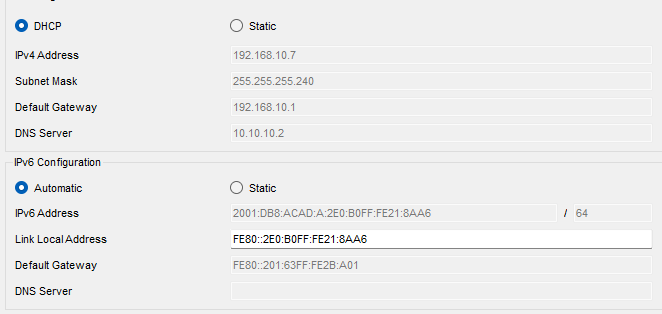
\includegraphics[width=16cm, height=14cm]{img/4.13.1a.png}
    \caption{Các PC lấy DHCPv4 và DHCPv6 thành công}
    \label{hinh4131a}
\end{figure}
\subsubsection{Kiểm tra gửi gói tin}
\begin{figure}[H]
    \centering
    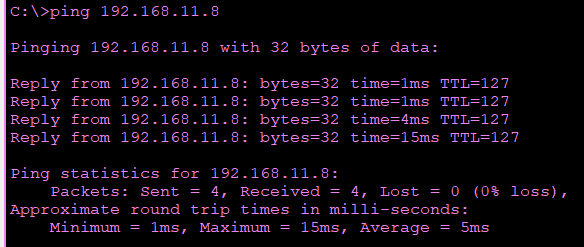
\includegraphics[width=16cm, height=14cm]{img/4.13.1c.png}
    \caption{Các VLAN ping với nhau bằng IPv4 thành công }
    \label{hinh4131c}
\end{figure}

\begin{figure}[H]
    \centering
    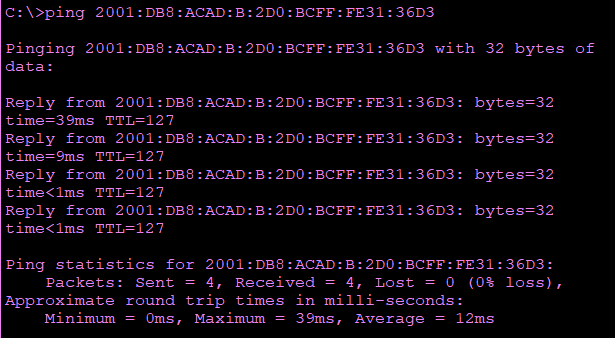
\includegraphics[width=16cm, height=14cm]{img/4.13.1d.png}
    \caption{Các VLAN ping với nhau bằng IPv6 thành công }
    \label{hinh4131d}
\end{figure}
\subsubsection{Kiểm tra ACL}

\begin{figure}[H]
    \centering
    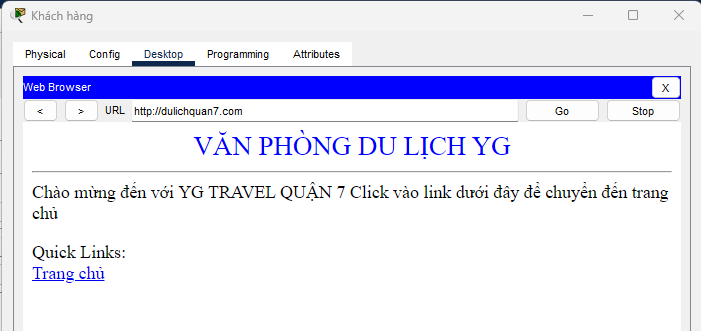
\includegraphics[width=16cm, height=14cm]{img/4.13.1b.png}
    \caption{Khách hàng truy cập được web }
    \label{hinh4131b}
\end{figure}


\begin{figure}[H]
    \centering
    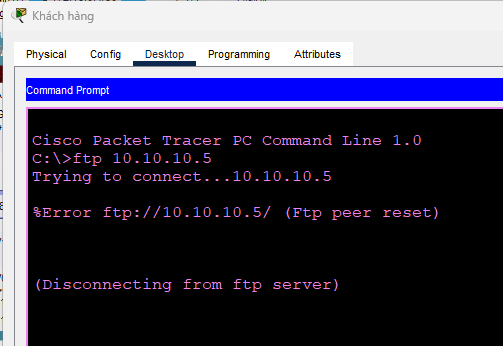
\includegraphics[width=16cm, height=14cm]{img/4.13.1e.png}
    \caption{Khách hàng không truy cập dịch vụ FTP }
    \label{hinh4131e}
\end{figure}


\begin{figure}[H]
    \centering
    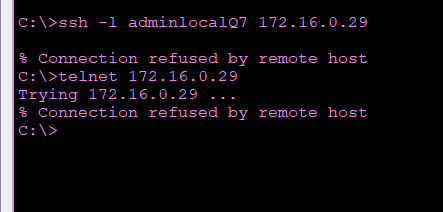
\includegraphics[width=16cm, height=14cm]{img/4.13.1f.png}
    \caption{Khách hàng không thể Telnet/SSH đến các thiết bị trong công ti }
    \label{hinh4131f}
\end{figure}



\begin{figure}[H]
    \centering
    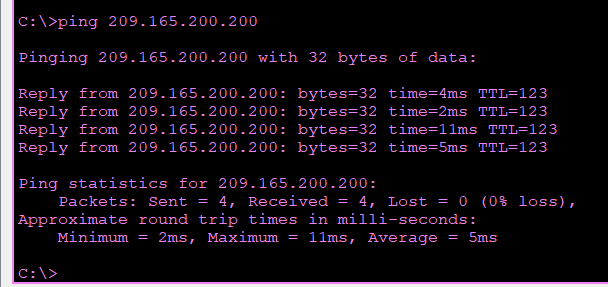
\includegraphics[width=16cm, height=14cm]{img/4.13.1g.png}
    \caption{Khi ping đến OUTSIDE thì cho phép OUTSIDE reply }
    \label{hinh4131g}
\end{figure}



\begin{figure}[H]
    \centering
    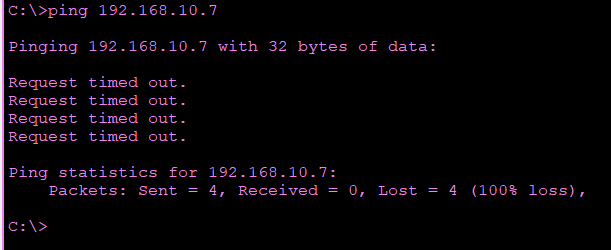
\includegraphics[width=16cm, height=14cm]{img/4.13.1h.png}
    \caption{Nhưng OUTSIDE không thể ping vào trong công ty}
    \label{hinh4131h}
\end{figure}

\subsubsection{Kiểm tra dịch vụ NTP và Syslog }
\begin{figure}[H]
    \centering
    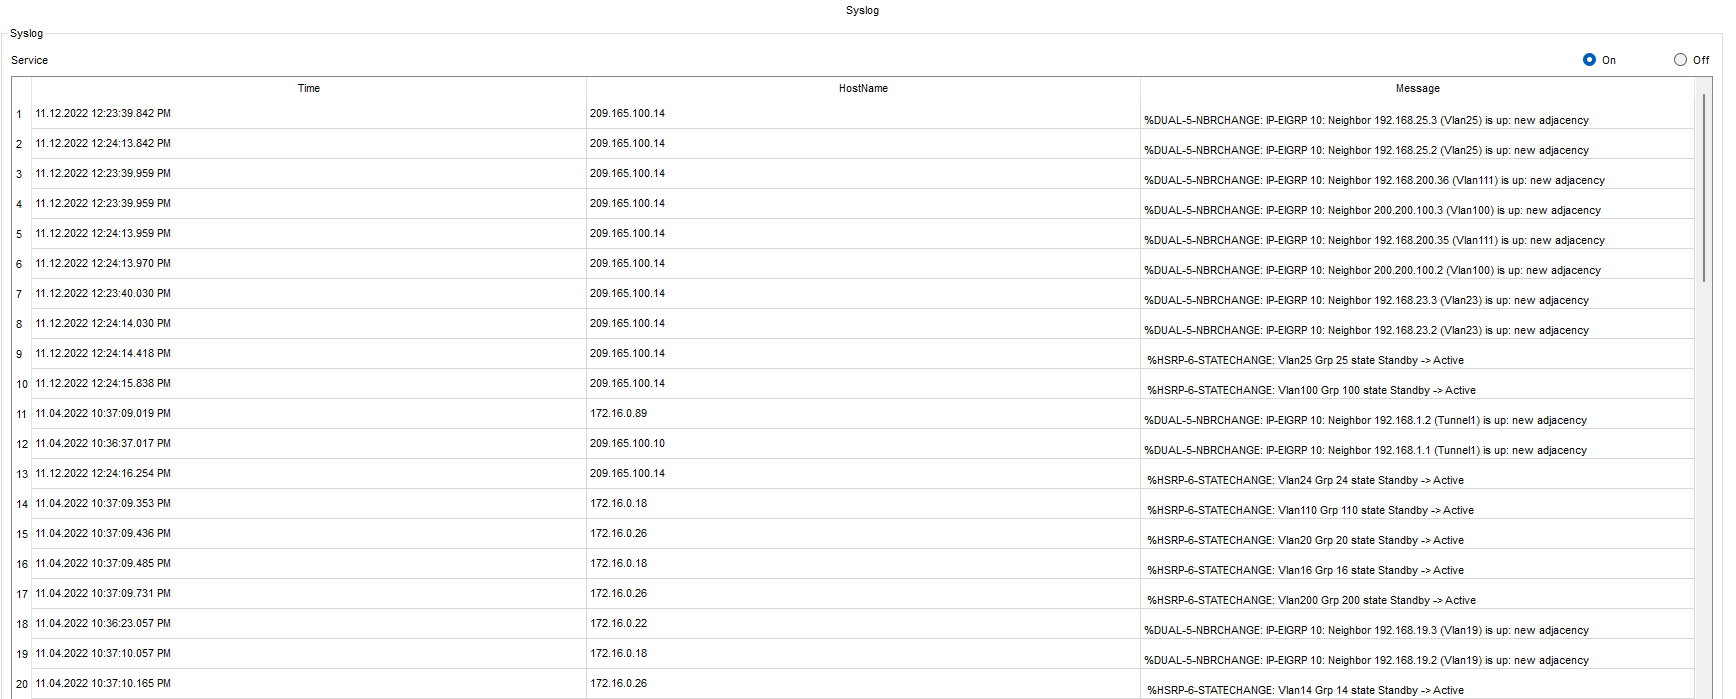
\includegraphics[width=16cm, height=14cm]{img/4.13.1i.png}
    \caption{Syslog Server ghi lại nhật ký đăng nhập vào các thiết bị }
    \label{hinh4131i}
\end{figure}

\subsubsection{Kiểm tra backup}
\begin{figure}[H]
    \centering
    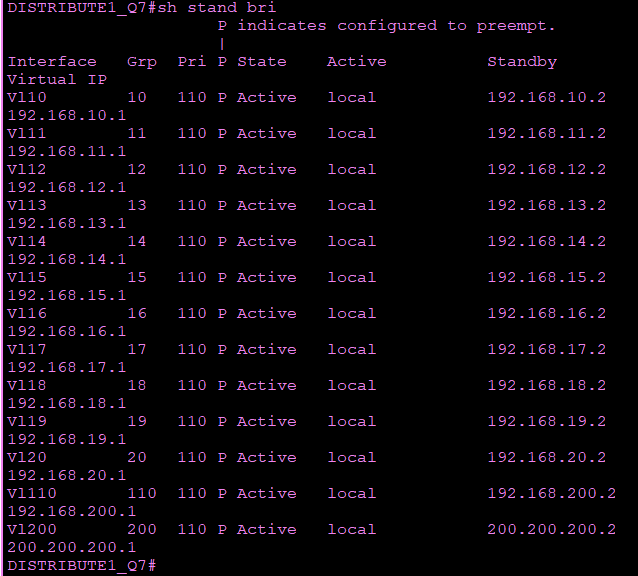
\includegraphics[width=16cm, height=14cm]{img/4.13.1j.png}
    \caption{Cấu hình HSRP trên Distribution 1 ở trạng thái acitve}
    \label{hinh4131j}
\end{figure}

\begin{figure}[H]
    \centering
    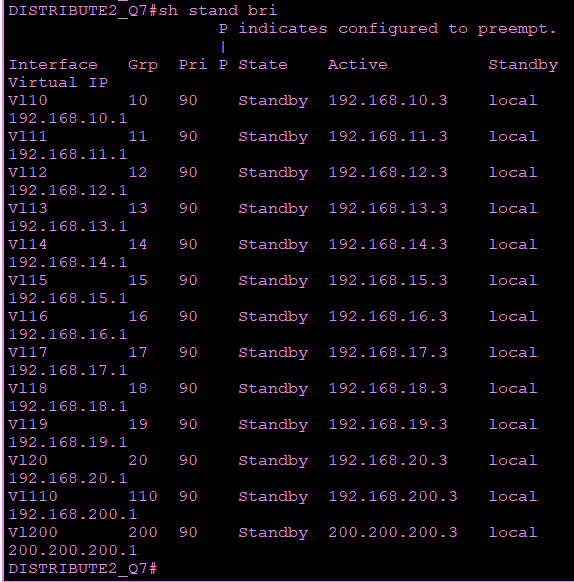
\includegraphics[width=16cm, height=14cm]{img/4.13.2a.png}
    \caption{Cấu hình HSRP trên Distribution 1 ở trạng thái stanby}
    \label{hinh4132a}
\end{figure}

\begin{figure}[H]
    \centering
    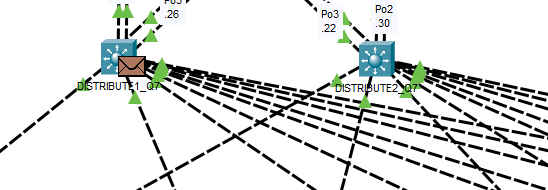
\includegraphics[width=16cm, height=6cm]{img/4.13.2b.png}
    \caption{Khi Switch Distribution 1 hoạt động bình thường, nó sẽ chiếm quyền gửi gói tin }
    \label{hinh4132b}
\end{figure}

\begin{figure}[H]
    \centering
    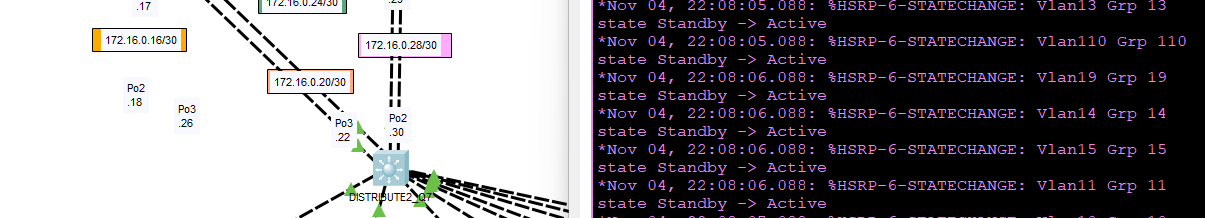
\includegraphics[width=16cm, height=5cm]{img/4.13.2c.png}
    \caption{Khi Distribution 1 bị hư, Distribution 2 sẽ đứng lên chiếm quyền }
    \label{hinh4132c}
\end{figure}

\begin{figure}[H]
    \centering
    \includegraphics[width=16cm, height=6cm]{img/4.13.2d.png}
    \caption{Khi này các gói tin gửi đi sẽ đi qua Distribution 2}
    \label{hinh4132d}
\end{figure}
\subsubsection{Kiểm tra Wifi}
\begin{figure}[H]
    \centering
    \includegraphics[width=16cm, height=14cm]{img/4.13.2e.png}
    \caption{Các thiết bị không dây kết nối wifi thành công}
    \label{hinh4132e}
\end{figure}

\begin{figure}[H]
    \centering
    \includegraphics[width=16cm, height=14cm]{img/4.13.2f.png}
    \caption{Thiết bị kết nối với WLAN nào thì sẽ nhận DHCP tương ứng}
    \label{hinh4132f}
\end{figure}
\subsubsection{Kiểm tra Port Security}
\begin{figure}[H]
    \centering
    \includegraphics[width=16cm, height=10cm]{img/po1.png}
    \caption{Port F0/1 mặc định của máy Lễ tân}
    \label{hinhstp1}
\end{figure}

\begin{figure}[H]
    \centering
    \includegraphics[width=16cm, height=10cm]{img/po2.png}
    \caption{Port F0/1 khi nối thiết bị khác}
    \label{hinhstp2}
\end{figure}


\subsubsection{Kiểm tra SSH Access}
\hspace*{0.25cm}Phòng kỹ thuật của trụ sở quận 7 có quyền truy cập SSH vào tất cả các thiết bị ở cả hai chi nhánh. Trong khi đó phòng kỹ thuật ở chi nhánh Thủ Đức chỉ có thể truy cập SSH vào các thiết bị ở Thủ Đức.\\
\begin{figure}[H]
    \centering
    \includegraphics[width=16cm, height=5cm]{img/ssh1.png}
    \caption{Phòng Kỹ thuật ở quận 7 có thể truy cập SSH vào các thiết bị ở quận 7}
    \label{hinhhsrp2}
\end{figure}
\begin{figure}[H]
    \centering
    \includegraphics[width=16cm, height=5cm]{img/ssh2.png}
    \caption{Phòng Kỹ thuật ở quận 7 có thể truy cập SSH vào các thiết bị ở Thủ Đức}
    \label{ssh2}
\end{figure}
\begin{figure}[H]
    \centering
    \includegraphics[width=16cm, height=6cm]{img/ssh3.png}
    \caption{Phòng Kỹ thuật ở Thủ Đức có thể truy cập SSH vào các thiết bị ở Thủ Đức}
    \label{ssh3}
\end{figure}
\begin{figure}[H]
    \centering
    \includegraphics[width=16cm, height=6cm]{img/ssh4.png}
    \caption{Phòng Kỹ thuật ở Thủ Đức không thể truy cập SSH vào các thiết bị ở quận 7}
    \label{ssh4}
\end{figure}
\subsubsection{Kiểm tra VPN-IPsec}
\begin{figure}[H]
    \centering
    \includegraphics[width=16cm, height=3cm]{img/vpn1.png}
    \caption{Hai VLAN hai chi nhánh ping thành công}
    \label{vpn1}
\end{figure}
\begin{figure}[H]
    \centering
    \includegraphics[width=16cm, height=12cm]{img/vpn2.png}
    \caption{Mạng VLAN đi qua tunnel}
    \label{vpn2}
\end{figure}
\subsubsection{Kiểm tra NAT}
\hspace*{0.25cm}Các VLAN kết nối ra outside sẽ được NAT\\
\begin{figure}[H]
    \centering
    \includegraphics[width=16cm, height=0.5cm]{img/natout.png}
    \caption{VLAN đi ra OUTSIDE thành công}
    \label{nat1}
\end{figure}
\begin{figure}[H]
    \centering
    \includegraphics[width=16cm, height=10cm]{img/nat1.png}
    \caption{Kiểm tra NAT trên R1}
    \label{nat1}
\end{figure}
\begin{figure}[H]
    \centering
    \includegraphics[width=16cm, height=10cm]{img/nat2.jpg}
    \caption{Kiểm tra NAT trên R2}
    \label{nat2}
\end{figure}
\begin{figure}[H]
    \centering
    \includegraphics[width=16cm, height=10cm]{img/nat3.jpg}
    \caption{Kiểm tra NAT trên R3}
    \label{nat3}
\end{figure}
\begin{figure}[H]
    \centering
    \includegraphics[width=16cm, height=10cm]{img/nat4.jpg}
    \caption{Kiểm tra NAT trên R4}
    \label{nat4}
\end{figure}
\subsubsection{Kiểm tra QoS Concept}
\begin{figure}[H]
    \centering
    \includegraphics[width=16cm, height=14cm]{img/qos1.png}
    \caption{kiểm tra QoS của các traffic}
    \label{qos1}
\end{figure}
\begin{figure}[H]
    \centering
    \includegraphics[width=16cm, height=14cm]{img/qos2.png}
    \caption{kiểm tra QoS của các traffic}
    \label{qos2}
\end{figure}
\cleardoublepage

\section*{CHƯƠNG 5 - KẾT LUẬN}
\addcontentsline{toc}{section}{\numberline{}CHƯƠNG 5 - KẾT LUẬN}
\hspace*{0.25cm}Nhìn chung, mô hình hệ thống mạng cũng đã hoàn thiện. Toàn bộ hệ thống đã được thiết kế và cấu hình trên Cisco Packet Tracer. Mô hình đáp ứng được các yêu cầu mà khách hàng đưa ra như các máy có thể ping được với nhau trong cùng một vlan, có trang web, có thể gửi file, truy cập website thông qua mạng internet, có cấu hình HSRP và STP để dự phòng và chống lặp. Ngoài ra, các phòng chức năng cũng được cấu hình mạng không dây với cấu hình bảo mật WPA2- Enterprise, có cấu hình đầy đủ các chức năng bảo mật như tường lửa, access list, VPN-Ipsec, SSH access, DHCP Snooping và Port security.\\
\hspace*{1cm}Để mô hình hệ thống mạng được hoàn thiện hơn trong tương lai thì chúng ta cần phải nâng cấp tính bảo mật của mô hình. Thêm một số tính năng cần thiết như mở rộng thêm nhiều điểm truy cập, mở rộng mô hình thêm nhiều thiết bị hơn
\cleardoublepage

\section*{TÀI LIỆU THAM KHẢO}
\addcontentsline{toc}{section}{\numberline{}TÀI LIỆU THAM KHẢO}
\hspace*{0.25cm}[1] Configuring DHCPv6 (both stateless and stateful) in Packet Tracer. (n.d.). Computernetworking. Retrieved May 27, 2022, from \\https://computernetworking747640215.wordpress.com/2019/11/05/configuring-dhcpv6-both-stateless-and-stateful-in-packet-tracer/\\
\hspace*{1cm}[2] Cấu hình HSRP CISCO. (n.d.). Https://Securityzone.Vn/. Retrieved May 27, 2022, from https://securityzone.vn/t/lab-13-cau-hinh-hsrp-cisco.182/\\

\cleardoublepage

\section*{PHỤ LỤC}
\addcontentsline{toc}{section}{\numberline{}PHỤ LỤC}
\hspace*{0.25cm}[1] \textbf{Password console }: dulichquan7\\
\hspace*{1cm}[2] \textbf{Password console }: dulichthuduc\\
\hspace*{1cm}[3] \textbf{Password enable} : vanphongcongtidulichquan7\\
\hspace*{1cm}[4] \textbf{Password enable} : vanphongcongtidulichthuduc\\
\hspace*{1cm}[5] \textbf{Account truy cập SSH LOCAL }: username : adminlocalQ7  , password : dulichcompanyquan7 \\
\hspace*{1cm}[6] \textbf{Account truy cập SSH LOCAL }: username : adminlocalTD  , password : dulichcompanythuduc\\
\hspace*{1cm}[7] \textbf{Account truy cập SSH CENTRAL}: username : admincentralQ7  , password : dulichcompanyquan7 \\
\hspace*{1cm}[8] \textbf{Account truy cập SSH CENTRAL }: username : admincentralTD  , password : dulichcompanythuduc\\
\hspace*{1cm}[9] \textbf{Domain name} : dulichquan7.com\\
\hspace*{1cm}[10] \textbf{Domain name} : dulichthuduc.com\\
\hspace*{1cm}[11] \textbf{Account FTP } : username : admin , password: 123456\\
\hspace*{1cm}[12] \textbf{Password truy cập vào WLC } :\\
\hspace*{2cm} WLC\_Q7 : https://192.168.200.4, user: admin , password: Cisco123\\
\hspace*{2cm} WLC\_TD :https://192.168.200.34, user: admin,  password: Cisco123\\
\hspace*{1cm}[13] \textbf{Password vtp Q7}: dulichquan7\\
\hspace*{1cm}[14] \textbf{Password vtp TD}: dulichthuduc\\
\cleardoublepage
\end{document}